% Compilacion: usar la misma receta de LaTeX Workshop que tus otros archivos.
% !TeX encoding = UTF-8
% Tratado autonomo: figuras TikZ/PGFPlots, sin archivos externos.
% MiKTeX + VS Code: pdfLaTeX tres veces o latexmk -pdf.
% Unidades de estudio que comienzan en una pagina nueva.
\documentclass[11pt,a4paper]{article}
\usepackage[utf8]{inputenc}
\usepackage[T1]{fontenc}
\usepackage{lmodern}
\IfFileExists{spanish.ldf}{\usepackage[spanish,es-nodecimaldot,es-noquoting]{babel}}{}
\usepackage[a4paper,margin=1.8cm,headheight=15pt,footskip=23pt]{geometry}
\usepackage{amsmath,amssymb,amsthm,mathtools,bm}
\usepackage{microtype,booktabs,array,longtable,multicol,enumitem}
\usepackage[dvipsnames]{xcolor}
\usepackage{tikz,pgfplots,tikz-3dplot}
\usetikzlibrary{arrows.meta,calc,positioning,patterns,babel}
\usepgfplotslibrary{fillbetween,groupplots}
\pgfplotsset{compat=1.18}
\usepackage[most]{tcolorbox}
\usepackage{float,caption,fancyhdr,needspace,listings}
\usepackage[colorlinks=true,linkcolor=MidnightBlue,urlcolor=MidnightBlue]{hyperref}
\hypersetup{pdftitle={Esperanza, varianza y covarianza: de escalares a matrices, PCA, SVD, MCO, IV y SVR},pdfauthor={Tratado matematico de estudio},pdfsubject={Probabilidad, algebra lineal, calculo matricial y estimadores}}
\definecolor{azul}{RGB}{21,64,112}
\definecolor{celeste}{RGB}{235,244,252}
\definecolor{rojo}{RGB}{181,58,58}
\definecolor{verde}{RGB}{27,119,94}
\definecolor{gris}{RGB}{83,94,108}
\pagestyle{fancy}\fancyhf{}
\fancyhead[L]{\small\color{azul}Esperanza, varianza y covarianza}
\fancyhead[R]{\small\color{gris}Álgebra, probabilidad y estimación}
\fancyfoot[C]{\small\thepage}
\setlength{\parindent}{0pt}\setlength{\parskip}{4pt}
\setlength{\abovedisplayskip}{6pt}\setlength{\belowdisplayskip}{6pt}
\setlength{\abovedisplayshortskip}{4pt}\setlength{\belowdisplayshortskip}{4pt}
\setlist{nosep,leftmargin=*}
\allowdisplaybreaks[2]\emergencystretch=2em
\captionsetup{font=small,labelfont=bf,skip=4pt}
\renewcommand{\figurename}{Figura}\renewcommand{\tablename}{Cuadro}
\newcommand{\R}{\mathbb R}
\newcommand{\N}{\mathbb N}
\newcommand{\E}{\mathbb E}
\newcommand{\Prob}{\mathbb P}
\newcommand{\T}{^{\mathsf T}}
\newcommand{\dd}{\,\mathrm d}
\newcommand{\ind}{\mathbf 1}
\newcommand{\ones}{\mathbf 1}
\newcommand{\norm}[1]{\left\lVert #1\right\rVert}
\newcommand{\abs}[1]{\left\lvert #1\right\rvert}
\newcommand{\ip}[2]{\left\langle #1,#2\right\rangle}
\DeclareMathOperator{\Var}{Var}
\DeclareMathOperator{\Cov}{Cov}
\DeclareMathOperator{\Corr}{Corr}
\DeclareMathOperator{\tr}{tr}
\DeclareMathOperator{\rank}{rank}
\DeclareMathOperator{\diag}{diag}
\DeclareMathOperator{\vecop}{vec}
\DeclareMathOperator{\spanop}{span}
\DeclareMathOperator{\sign}{sign}
\DeclareMathOperator*{\argmin}{arg\,min}
\DeclareMathOperator*{\argmax}{arg\,max}
\newcommand{\pto}{\xrightarrow{\Prob}}
\newcommand{\dto}{\xrightarrow{\mathrm d}}
\newcommand{\Normal}{\mathcal N}
\newcommand{\op}{_{\mathrm{op}}}
\newcommand{\F}{_{\mathrm F}}
\newcommand{\topic}[2]{\clearpage\section{#1}\label{#2}}
\newcommand{\ruta}[2]{\hyperref[#1]{\ref{#1}. #2}\dotfill\pageref{#1}\par}
\newtcolorbox{idea}[1][]{enhanced,breakable,colback=celeste,colframe=azul,boxrule=.5pt,arc=1mm,left=6pt,right=6pt,top=4pt,bottom=4pt,title={#1},fonttitle=\bfseries}
\newtcolorbox{ejemplo}[1][]{enhanced,breakable,colback=white,colframe=verde,boxrule=.5pt,arc=1mm,left=6pt,right=6pt,top=4pt,bottom=4pt,title={#1},fonttitle=\bfseries}
\newtcolorbox{cuidado}[1][]{enhanced,breakable,colback=red!2,colframe=rojo,boxrule=.5pt,arc=1mm,left=6pt,right=6pt,top=4pt,bottom=4pt,title={#1},fonttitle=\bfseries}
\newenvironment{deduccion}{\par\textbf{Deducción.}\ }{\hfill$\square$\par}
\newtheorem{teorema}{Teorema}[section]
\newtheorem{proposicion}[teorema]{Proposición}
\theoremstyle{definition}\newtheorem{definicion}[teorema]{Definición}
\pgfplotsset{base/.style={axis lines=left,grid=both,grid style={gray!15},tick label style={font=\scriptsize},label style={font=\small},legend style={font=\scriptsize,draw=none,fill=white},samples=110},curva/.style={very thick,azul}}
\tikzset{vec/.style={-{Latex[length=2.3mm]},very thick,azul},eje/.style={-{Latex[length=1.8mm]},gray},vverde/.style={-{Latex[length=2.3mm]},very thick,verde}}
\lstset{basicstyle=\ttfamily\footnotesize,breaklines=true,frame=single,backgroundcolor=\color{celeste!35},columns=fullflexible,keepspaces=true,showstringspaces=false}
\pdfstringdefDisableCommands{\def\T{ T}\def\E{E}\def\Var{Var}\def\Cov{Cov}\def\Sigma{Sigma}\def\beta{beta}\def\R{R}}
\begin{document}
\thispagestyle{empty}
\begin{center}
{\Huge\bfseries\color{azul}Esperanza, varianza\\[3pt]y covarianza}\\[10pt]
{\LARGE De escalares a vectores y matrices}\\[7pt]
{\Large Normal multivariada, PCA, SVD, MCO, IV y SVR}\\[8pt]
{\large Tratado matemático con deducciones y ejemplos completos}\\[4pt]
\textit{Probabilidad + álgebra lineal + cálculo matricial + estimación}
\end{center}
\begin{idea}[La operación central: centrar, multiplicar y promediar]
Para un vector aleatorio $x\in\R^{p\times1}$ con segundo momento finito,
\[
\mu=\E[x],\qquad
\boxed{\Sigma=\Cov(x)=\E[(x-\mu)(x-\mu)\T]\in\R^{p\times p}}.
\]
La matriz conserva simultáneamente todas las varianzas y covarianzas:
\[
\Sigma_{ij}=\E[(x_i-\mu_i)(x_j-\mu_j)],\qquad
\boxed{\Cov(Ax+b)=A\Sigma A\T}.
\]
Esta identidad explicará la incertidumbre de combinaciones, proyecciones,
coeficientes de regresión y predicciones. Su deducción no requiere normalidad.
\end{idea}
\begin{center}
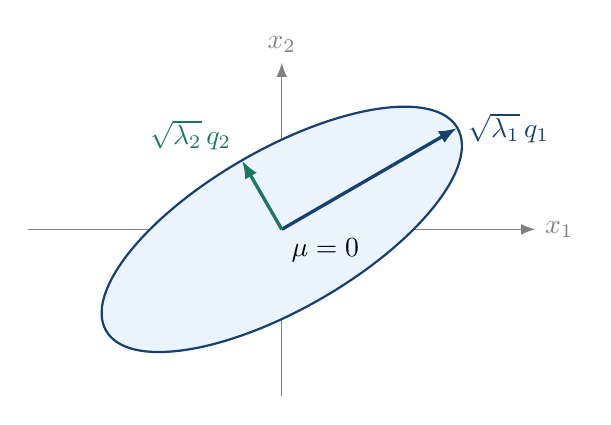
\begin{tikzpicture}[scale=.92]
\draw[eje](-3.5,0)--(3.5,0)node[right]{$x_1$};
\draw[eje](0,-2.3)--(0,2.3)node[above]{$x_2$};
\draw[rotate=30,azul,fill=celeste,thick](0,0)ellipse(2.8 and 1.1);
\draw[vec](0,0)--(2.42,1.4)node[right]{$\sqrt{\lambda_1}\,q_1$};
\draw[vverde](0,0)--(-.55,.953)node[above left]{$\sqrt{\lambda_2}\,q_2$};
\node[below right] at (0,0){$\mu=0$};
\end{tikzpicture}
\end{center}
\textbf{Ruta de aprendizaje.} Comenzamos con sumas e integrales de distribuciones
elementales. Construimos después los operadores de momentos, las formas
cuadráticas y la normal multivariada. Solo entonces estimamos medias,
covarianzas, componentes principales y coeficientes de regresión.

\textbf{Nivel y alcance.} Se desarrolla cada resultado central con sus
hipótesis, dimensiones y pasos algebraicos. Los teoremas de límite se
justifican bajo condiciones explícitas; no se presenta una aproximación
asintótica como una identidad de muestra finita. En SVR e IV, la existencia
de momentos merece tanta atención como su cálculo.

\textbf{Código autónomo.} Las figuras son vectoriales y forman parte de este
archivo. Usa pdfLaTeX con paquetes estándar de MiKTeX. No hacen falta
imágenes externas, Python, Bib\TeX{} ni \texttt{shell-escape}.
\clearpage
\section*{Índice I: probabilidad, operadores y geometría}
\small
\ruta{s01}{Probabilidad y definición de distribución}
\ruta{s02}{Bernoulli y binomial: momentos desde indicadores}
\ruta{s03}{Poisson y geométrica: derivar usando series}
\ruta{s04}{Uniforme, exponencial y gamma: integrar momentos}
\ruta{s05}{Normal escalar: integral gaussiana y momentos}
\ruta{s06}{Chi-cuadrado, Student, F y colas sin momentos}
\ruta{s07}{Esperanza: un operador lineal sobre funciones}
\ruta{s08}{Varianza escalar: operador cuadrático}
\ruta{s09}{Covarianza escalar, Cauchy--Schwarz y dependencia}
\ruta{s10}{Condicionar: torre y descomposición de momentos}
\ruta{s11}{Álgebra lineal: dimensiones, traza y productos}
\ruta{s12}{Esperanza y covarianza vectorial}
\ruta{s13}{Positividad, rango y direcciones deterministas}
\ruta{s14}{Ejemplo de tres variables con factores comunes}
\ruta{s15}{Cálculo vectorial: gradiente, Hessiana y Taylor}
\ruta{s16}{Diferenciales matriciales, inversa y determinante}
\ruta{s17}{Proyección en L2 y mejor predicción lineal}
\ruta{s18}{Matrices aleatorias, vectorización y Kronecker}
\ruta{s19}{Construcción y densidad de la normal multivariada}
\ruta{s20}{Momentos gaussianos y formas cuadráticas}
\ruta{s21}{Normal condicional y complemento de Schur}
\ruta{s22}{Elipsoides, blanqueamiento y Mahalanobis}
\ruta{s23}{Media muestral, dependencia y ley de grandes números}
\ruta{s24}{Covarianza muestral: por qué aparece n menos uno}
\ruta{s25}{Wishart y covarianza entre covarianzas}
\ruta{s26}{Muchas dimensiones: singularidad y regularización}
\ruta{s27}{Teorema espectral y cociente de Rayleigh}
\ruta{s28}{PCA: máxima varianza y mínima reconstrucción}
\normalsize
\begin{idea}[Contrato de dimensiones]
$x\in\R^p$ es un vector aleatorio; $D\in\R^{n\times p}$ es una tabla de datos
para PCA; $X\in\R^{n\times k}$ es el diseño de regresión e incluye el
intercepto cuando se indique. $Z\in\R^{n\times\ell}$ contiene instrumentos.
$\mu,\Sigma$ son momentos poblacionales; $\bar x,S$ son estimadores.
\[
y=X\beta+u,\quad
y,u\in\R^n,\ \beta\in\R^k,\qquad
\Cov(u\mid X)=\Omega\in\R^{n\times n}.
\]
Una letra mayúscula no implica por sí sola aleatoriedad. Cada sección indica
qué cantidades se fijan y sobre cuáles se toma la esperanza.
\end{idea}
\textbf{Convenciones.} Todos los vectores son columnas; $A\T$ es la transpuesta,
$I_d$ la identidad de orden $d$, $\ones$ el vector de unos y $\delta_{ij}$ vale
uno si $i=j$ y cero en caso contrario. \emph{iid} significa independientes e
idénticamente distribuidos. $\pto$ expresa convergencia en probabilidad y
$\dto$ convergencia en distribución.
\clearpage
\section*{Índice II: estimadores y aprendizaje automático}
\small
\ruta{s29}{SVD, pseudoinversa y aproximación de rango bajo}
\ruta{s30}{Laboratorio exacto de PCA y SVD}
\ruta{s31}{Incertidumbre de autovalores y autovectores}
\ruta{s32}{PCR y ridge: esperanza, sesgo y covarianza}
\ruta{s33}{MCO desde la función objetivo}
\ruta{s34}{Momentos de todos los coeficientes MCO}
\ruta{s35}{Gauss--Markov y diseño aleatorio}
\ruta{s36}{Residuos, varianza del error, Student y F}
\ruta{s37}{Contrastes, predicciones y funciones de coeficientes}
\ruta{s38}{MCO numérico: cada operación y cada covarianza}
\ruta{s39}{Heterocedasticidad, covarianza robusta y clústeres}
\ruta{s40}{GLS: blanquear errores y ganar eficiencia}
\ruta{s41}{Regresión multivariada y matriz de coeficientes}
\ruta{s42}{CLT vectorial, método delta y sándwich}
\ruta{s43}{Endogeneidad e identificación instrumental}
\ruta{s44}{IV exacto: cocientes y momentos de muestra finita}
\ruta{s45}{2SLS: deducción de las dos etapas}
\ruta{s46}{Covarianza asintótica de 2SLS}
\ruta{s47}{GMM y ponderación eficiente de momentos}
\ruta{s48}{IV numérico: MCO, 2SLS y errores estructurales}
\ruta{s49}{SVR: pérdida insensible y objetivo poblacional}
\ruta{s50}{SVR primal, dual y condiciones KKT}
\ruta{s51}{Núcleos, Gram y representación de SVR}
\ruta{s52}{SVR numérico: solución primal y dual}
\ruta{s53}{SVR: momentos exactos en un modelo resoluble}
\ruta{s54}{SVR: sándwich asintótico y remuestreo}
\ruta{s55}{Normal bayesiana, posterior y conexión con ridge}
\ruta{s56}{Taller de integración y mapa de fórmulas}
\normalsize
\begin{cuidado}[Tres objetos que conviene separar desde el principio]
Un \textbf{parámetro} $\beta$ es fijo en la interpretación frecuentista.
El \textbf{estimador} $\widehat\beta=T(X,y)$ es aleatorio antes de observar la
muestra. La \textbf{estimación} es el valor numérico obtenido al aplicar $T$
a los datos concretos.
\[
\E[\widehat\beta],\quad
\Cov(\widehat\beta),\quad
\E[(\widehat\beta-\beta)(\widehat\beta-\beta)\T]
\]
son objetos diferentes. El tercero incluye el producto exterior del sesgo:
\[
\operatorname{MSE}_{\mathrm{mat}}
=\Cov(\widehat\beta)
+\{\E[\widehat\beta]-\beta\}\{\E[\widehat\beta]-\beta\}\T.
\]
\end{cuidado}
\textbf{Uso de las figuras.} Las curvas y superficies ilustran funciones
definidas en el texto. Los ejemplos numéricos pequeños permiten comprobar
las identidades sin depender de software. Los resultados generales usan
$p$, $k$ o $\ell$ arbitrarios: una demostración matricial no se limita al
número de coordenadas que podemos dibujar.

\textbf{Cómo seguir una deducción.} Comprueba primero las dimensiones.
Identifica después las hipótesis de existencia de momentos, independencia,
exogeneidad o normalidad. Expande finalmente el producto o la derivada antes
de aplicar una identidad abreviada. Las referencias primarias aparecen al
final, junto con las instrucciones de compilación.
\topic{Probabilidad y definición de distribución}{s01}
Un experimento produce un resultado $\omega$ dentro de un conjunto $\mathcal
\Omega$. Un evento $A$ es un conjunto de resultados, y una probabilidad
asigna un número $\Prob(A)\in[0,1]$, con $\Prob(\mathcal\Omega)=1$. Para eventos
disjuntos, la probabilidad de su unión es la suma de sus probabilidades.
Una variable aleatoria real $U$ es una función $\omega\mapsto U(\omega)$:
convierte resultados en números.
\[
F_U(t)=\Prob(U\le t),\qquad
\Prob(a<U\le b)=F_U(b)-F_U(a).
\]
$F_U$ es creciente, continua por la derecha, y tiende a cero y uno en los
extremos. En el caso discreto, $p_j=\Prob(U=u_j)$ y $\sum_jp_j=1$.
En el caso con densidad,
\[
f_U(u)\ge0,\quad\int_{\R}f_U(u)\dd u=1,\qquad
F_U(t)=\int_{-\infty}^t f_U(u)\dd u.
\]
Una densidad es masa \emph{por unidad de longitud}; puede superar uno. Una
probabilidad de intervalo es una integral, no el valor puntual de $f_U$.

\begin{definicion}[Integrar respecto de una distribución]
Para una función $g$ que cumple $\E[\abs{g(U)}]<\infty$, definimos
\[
\E[g(U)]=\int_{\R}g(u)\dd F_U(u)
=\begin{cases}
\sum_jg(u_j)p_j,&\text{discreta},\\
\int_{\R}g(u)f_U(u)\dd u,&\text{con densidad}.
\end{cases}
\]
La notación $\dd F_U$ incluye distribuciones discretas, continuas y mixtas.
\end{definicion}
El momento de orden $r$ es $m_r=\E[U^r]$ cuando existe como integral absoluta.
La media es $\mu=m_1$ y el momento central de orden $r$ es $\E[(U-\mu)^r]$.
Para el segundo orden,
\[
\E[U^2]<\infty\ \Longrightarrow\
\E[\abs U]\le\sqrt{\E[U^2]}<\infty.
\]
La desigualdad se demostrará mediante Cauchy--Schwarz. Por ello, un segundo
momento finito basta para definir media, varianza y covarianzas.

\begin{ejemplo}[Una distribución que se puede comprobar a mano]
$U$ toma $-1,0,2$ con probabilidades $1/4,1/2,1/4$. Entonces
\[
\E[U]=-\frac14+0+\frac24=\frac14,\qquad
\E[U^2]=\frac14+0+\frac44=\frac54,
\]
\[
\E[(U-\tfrac14)^2]
=\frac14\frac{25}{16}+\frac12\frac1{16}
+\frac14\frac{49}{16}=\frac{19}{16}.
\]
Así, $\Var(U)=19/16$, mientras que el segundo momento es $20/16$.
\end{ejemplo}
\textbf{Transformar no cambia las probabilidades originales.}
Para $V=g(U)$, $\Prob(V\in B)=\Prob(U\in g^{-1}(B))$.
Si $g$ es diferenciable e invertible en un intervalo,
\[
f_V(v)=f_U(g^{-1}(v))\abs{\frac{\dd g^{-1}(v)}{\dd v}}.
\]
El valor absoluto del Jacobiano conserva la masa al cambiar coordenadas.
Cuando varias ramas de $g$ producen el mismo $v$, se suman sus contribuciones.
Esta idea reaparecerá al construir una normal en muchas dimensiones.

\topic{Bernoulli y binomial: momentos desde indicadores}{s02}
Sea $B=\ind_A$, el indicador de un evento de probabilidad $\pi$:
$B=1$ si ocurre $A$ y cero en otro caso. Su distribución es Bernoulli:
\[
\Prob(B=b)=\pi^b(1-\pi)^{1-b},\quad b\in\{0,1\}.
\]
Como $B^r=B$ para cualquier entero $r\ge1$,
\[
\E[B]=\pi,\quad \E[B^2]=\pi,\qquad
\Var(B)=\pi-\pi^2=\pi(1-\pi).
\]
La derivación directa confirma el resultado:
$\E[(B-\pi)^2]=\pi(1-\pi)^2+(1-\pi)\pi^2=\pi(1-\pi)$.
La varianza es cero cuando el resultado es seguro y máxima en $\pi=1/2$.

\textbf{Contar éxitos.} Para $m$ indicadores independientes con la misma
probabilidad $\pi$, sea $N=\sum_{j=1}^m B_j$. Exactamente $r$ éxitos pueden
situarse en $\binom mr=m!/[r!(m-r)!]$ subconjuntos, de modo que
\[
\Prob(N=r)=\binom mr\pi^r(1-\pi)^{m-r},\qquad r=0,\ldots,m.
\]
El binomio de Newton demuestra que estas probabilidades suman uno.

\begin{deduccion}
Por linealidad, $\E[N]=\sum_j\E[B_j]=m\pi$. Expandiendo el cuadrado,
\[
\E[N^2]=\sum_j\E[B_j^2]+2\sum_{i<j}\E[B_iB_j]
=m\pi+m(m-1)\pi^2.
\]
La independencia da $\E[B_iB_j]=\pi^2$. Restar $(m\pi)^2$ produce
\[
\boxed{\Var(N)=m\pi(1-\pi)}.
\]
Sin independencia, el cálculo correcto agrega las covarianzas:
$\Var(N)=\sum_j\Var(B_j)+2\sum_{i<j}\Cov(B_i,B_j)$.
\end{deduccion}

\begin{ejemplo}[Indicadores que comparten el mismo resultado]
Si $B_1=B_2=B$, entonces $N=2B$ y $\Var(N)=4\pi(1-\pi)$.
Usar la fórmula binomial daría $2\pi(1-\pi)$, porque eliminaría
incorrectamente $\Cov(B_1,B_2)=\pi(1-\pi)$.
\end{ejemplo}
\textbf{Función generadora de momentos.} Cuando es finita cerca de cero,
$M_U(t)=\E[e^{tU}]$. Para Bernoulli y para la suma independiente,
\[
M_B(t)=1-\pi+\pi e^t,\qquad
M_N(t)=\prod_{j=1}^mM_{B_j}(t)=(1-\pi+\pi e^t)^m.
\]
Al derivar bajo una suma finita, $M'_N(0)=\E[N]$ y
$M''_N(0)=\E[N^2]$. La función $K_U(t)=\log M_U(t)$ satisface
$K'_U(0)=\E[U]$ y $K''_U(0)=\Var(U)$.
\begin{figure}[H]\centering
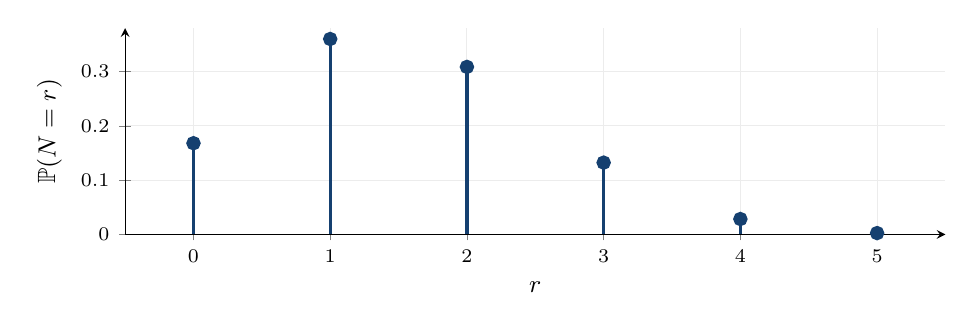
\begin{tikzpicture}
\begin{axis}[base,width=12cm,height=4.2cm,xmin=-.5,xmax=5.5,ymin=0,ymax=.38,xlabel={$r$},ylabel={$\Prob(N=r)$},xtick={0,...,5}]
\addplot[ycomb,mark=*,very thick,azul]coordinates{(0,.16807)(1,.36015)(2,.3087)(3,.1323)(4,.02835)(5,.00243)};
\end{axis}
\end{tikzpicture}
\caption{$N\sim\operatorname{Bin}(5,0.3)$: media $1.5$ y varianza $1.05$.}
\end{figure}

\topic{Poisson y geométrica: derivar usando series}{s03}
La distribución Poisson con intensidad $\lambda>0$ asigna
\[
\Prob(N=r)=e^{-\lambda}\frac{\lambda^r}{r!},\quad r=0,1,\ldots.
\]
La serie $e^\lambda=\sum_{r\ge0}\lambda^r/r!$ verifica la normalización.
Como $r/r!=1/(r-1)!$ para $r\ge1$,
\[
\E[N]=e^{-\lambda}\sum_{r=1}^\infty
\frac{r\lambda^r}{r!}
=\lambda e^{-\lambda}\sum_{s=0}^\infty\frac{\lambda^s}{s!}
=\lambda.
\]
Es más sencillo comenzar el segundo momento con un factorial descendente:
\[
\E[N(N-1)]
=e^{-\lambda}\sum_{r=2}^\infty\frac{r(r-1)\lambda^r}{r!}
=\lambda^2.
\]
Como $N^2=N(N-1)+N$, $\E[N^2]=\lambda^2+\lambda$ y
$\boxed{\Var(N)=\lambda}$. También
\[
M_N(t)=e^{-\lambda}\sum_{r\ge0}\frac{(\lambda e^t)^r}{r!}
=\exp\{\lambda(e^t-1)\}.
\]

\textbf{Esperar hasta el primer éxito.} Para ensayos Bernoulli independientes,
$G$ cuenta el ensayo del primer éxito, incluyendo ese ensayo:
\[
\Prob(G=r)=\pi(1-\pi)^{r-1},\qquad r=1,2,\ldots.
\]
Escribamos $q=1-\pi$. Derivando la serie geométrica dentro de $\abs q<1$,
\[
\sum_{r=1}^{\infty}rq^{r-1}=\frac1{(1-q)^2},\qquad
\sum_{r=1}^{\infty}r(r-1)q^{r-2}=\frac2{(1-q)^3}.
\]
Por tanto,
\[
\E[G]=\frac{\pi}{(1-q)^2}=\frac1\pi,\qquad
\E[G(G-1)]=\frac{2\pi q}{(1-q)^3}=\frac{2q}{\pi^2},
\]
\[
\E[G^2]=\frac{2q}{\pi^2}+\frac1\pi=\frac{2-\pi}{\pi^2},
\qquad \boxed{\Var(G)=\frac{1-\pi}{\pi^2}}.
\]
Si se cuentan solamente los fracasos $H=G-1$, la media cambia a
$(1-\pi)/\pi$ y la varianza se mantiene.

\begin{ejemplo}[Los mismos momentos no especifican la misma distribución]
Para $\lambda=2$, Poisson tiene media $2$ y varianza $2$.
Para $\pi=1/2$, $G$ también tiene media $2$ y varianza $2$.
Sin embargo, $\Prob(N=0)=e^{-2}>0$ y $\Prob(G=0)=0$.
Una media y una varianza no describen por completo una distribución.
\end{ejemplo}
\textbf{Ausencia de memoria.} La cola geométrica es
$\Prob(G>r)=q^r$. Entonces, para enteros $s,r\ge0$,
\[
\Prob(G>r+s\mid G>r)
=\frac{q^{r+s}}{q^r}=q^s=\Prob(G>s).
\]
Este resultado es una propiedad específica de la distribución, no una
consecuencia general de conocer sus dos primeros momentos.
Una suma de Poisson independientes es Poisson: sus funciones generadoras
se multiplican y las intensidades se suman. La independencia es esencial.

\topic{Uniforme, exponencial y gamma: integrar momentos}{s04}
Para $U\sim\operatorname{Unif}(a,b)$, $a<b$,
$f_U(u)=1/(b-a)$ dentro del intervalo y cero fuera. Integrar potencias da
\[
\E[U]=\frac1{b-a}\int_a^bu\dd u=\frac{a+b}{2},
\quad
\E[U^2]=\frac{b^3-a^3}{3(b-a)}=\frac{a^2+ab+b^2}{3},
\]
\[
\boxed{\Var(U)=\frac{(b-a)^2}{12}}.
\]
Con $a=0,b=1$, $\E[U^r]=1/(r+1)$ para $r>-1$. Si $U$ es uniforme
en $(0,1)$, $T=-\log U/\lambda$ cumple
$\Prob(T>t)=\Prob(U<e^{-\lambda t})=e^{-\lambda t}$ para $t\ge0$.

\textbf{Exponencial.} Para $T\sim\operatorname{Exp}(\lambda)$,
$f_T(t)=\lambda e^{-\lambda t}\ind_{\{t\ge0\}}$.
Integración por partes, con $u=t^r$ y $\dd v=\lambda e^{-\lambda t}\dd t$,
produce para enteros $r\ge1$
\[
\E[T^r]
=\left[-t^re^{-\lambda t}\right]_0^\infty
+r\int_0^\infty t^{r-1}e^{-\lambda t}\dd t
=\frac r\lambda\E[T^{r-1}].
\]
Partiendo de $\E[T^0]=1$, se obtiene
$\E[T^r]=r!/\lambda^r$; así, $\E[T]=1/\lambda$ y
$\Var(T)=2/\lambda^2-1/\lambda^2=1/\lambda^2$.

\textbf{Gamma con parámetro de tasa.} Definimos
$\Gamma(a)=\int_0^\infty t^{a-1}e^{-t}\dd t$ para $a>0$.
Por partes, $\Gamma(a+1)=a\Gamma(a)$ y $\Gamma(1)=1$.
La densidad
\[
f_V(v)=\frac{\lambda^a}{\Gamma(a)}v^{a-1}e^{-\lambda v}
\ind_{\{v>0\}}
\]
se normaliza con el cambio $t=\lambda v$. El mismo cambio en sus momentos
da, para $r>-a$,
\[
\E[V^r]=\frac{\Gamma(a+r)}{\Gamma(a)\lambda^r},
\qquad \boxed{\E[V]=a/\lambda,\quad \Var(V)=a/\lambda^2}.
\]
Su función generadora es $M_V(t)=(\lambda/(\lambda-t))^a$, $t<\lambda$.
La suma de $a$ exponenciales iid tiene esta distribución si $a$ es entero.

\begin{figure}[H]\centering
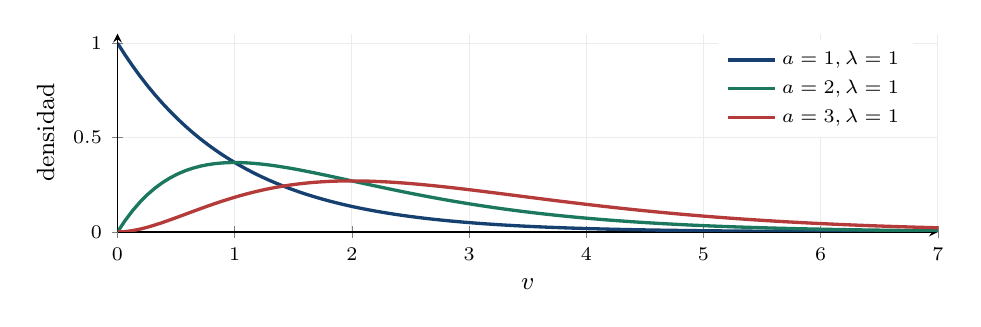
\begin{tikzpicture}
\begin{axis}[base,width=12cm,height=4.1cm,xmin=0,xmax=7,ymin=0,ymax=1.05,xlabel={$v$},ylabel={densidad},legend pos=north east]
\addplot[curva,domain=0:7]{exp(-x)};\addlegendentry{$a=1,\lambda=1$}
\addplot[verde,very thick,domain=0:7]{x*exp(-x)};\addlegendentry{$a=2,\lambda=1$}
\addplot[rojo,very thick,domain=0:7]{x*x*exp(-x)/2};\addlegendentry{$a=3,\lambda=1$}
\end{axis}
\end{tikzpicture}
\caption{Misma tasa, distintos parámetros de forma. Las integrales de las tres densidades son uno.}
\end{figure}
\begin{cuidado}[Tasa y escala]
Si $\theta=1/\lambda$ es la escala, las fórmulas son
$\E[V]=a\theta$ y $\Var(V)=a\theta^2$. Escribir solamente
$\operatorname{Gamma}(a,\lambda)$ sin declarar la convención puede invertir
todos los resultados.
\end{cuidado}

\topic{Normal escalar: integral gaussiana y momentos}{s05}
Sea $I=\int_{\R}e^{-z^2/2}\dd z$. Al multiplicar dos copias de esta
integral y pasar a coordenadas polares $(z_1,z_2)=(r\cos t,r\sin t)$,
el Jacobiano vale $r$ y
\[
I^2=\int_0^{2\pi}\int_0^\infty e^{-r^2/2}r\dd r\dd t=2\pi,
\quad I=\sqrt{2\pi}.
\]
Así, $\phi(z)=(2\pi)^{-1/2}e^{-z^2/2}$ es una densidad. Una variable
$Z$ con esa densidad es normal estándar. La simetría hace
$\E[Z^{2r+1}]=0$, y $\phi'(z)=-z\phi(z)$ permite integrar por partes:
\[
\E[Z^{2r}]
=-\int_{\R}z^{2r-1}\phi'(z)\dd z
=(2r-1)\int_{\R}z^{2r-2}\phi(z)\dd z.
\]
Los términos de frontera son cero porque el exponencial decrece más rápido
que cualquier potencia. Por recurrencia,
\[
\E[Z^2]=1,\qquad \E[Z^4]=3,\qquad
\E[Z^{2r}]=(2r-1)(2r-3)\cdots1.
\]

\textbf{Trasladar y escalar.} Para $\sigma>0$, $U=\mu+\sigma Z$ tiene
\[
f_U(u)=\frac1{\sigma\sqrt{2\pi}}
\exp\!\left\{-\frac{(u-\mu)^2}{2\sigma^2}\right\},
\qquad U\sim\Normal(\mu,\sigma^2).
\]
El factor $1/\sigma$ es el Jacobiano. De la definición,
$\E[U]=\mu$, $\Var(U)=\sigma^2$ y $\E[U^2]=\mu^2+\sigma^2$.

\textbf{Completar el cuadrado.} Como $tz-z^2/2=t^2/2-(z-t)^2/2$,
\[
M_Z(t)=\int_{\R}e^{tz}\phi(z)\dd z=e^{t^2/2},
\qquad
M_U(t)=\exp(\mu t+\tfrac12\sigma^2t^2).
\]
Para $L=e^U$ (lognormal), evaluar esta función en $t=1,2$ da
\[
\E[L]=e^{\mu+\sigma^2/2},\qquad
\Var(L)=e^{2\mu+\sigma^2}(e^{\sigma^2}-1).
\]
En particular, $\E[e^U]\ne e^{\E[U]}$ cuando $\sigma^2>0$.
\begin{figure}[H]\centering
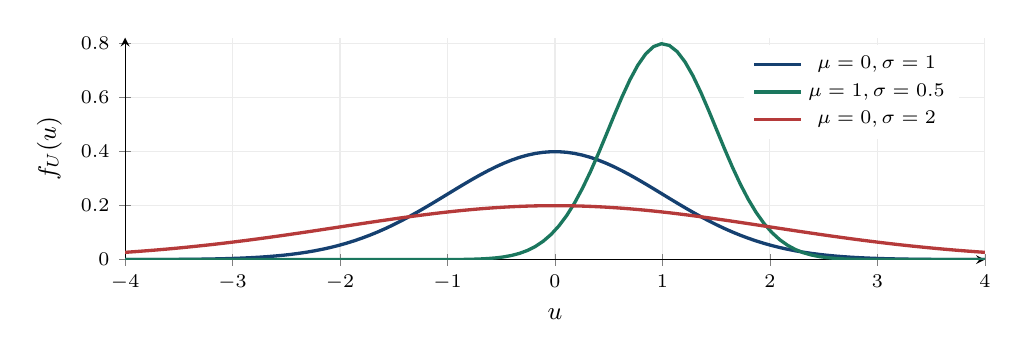
\begin{tikzpicture}
\begin{axis}[base,width=12.5cm,height=4.4cm,xmin=-4,xmax=4,ymin=0,ymax=.82,xlabel={$u$},ylabel={$f_U(u)$},legend pos=north east]
\addplot[curva,domain=-4:4]{exp(-x*x/2)/sqrt(2*pi)};\addlegendentry{$\mu=0,\sigma=1$}
\addplot[verde,very thick,domain=-4:4]{exp(-(x-1)^2/(.5))/sqrt(.5*pi)};\addlegendentry{$\mu=1,\sigma=0.5$}
\addplot[rojo,very thick,domain=-4:4]{exp(-x*x/8)/sqrt(8*pi)};\addlegendentry{$\mu=0,\sigma=2$}
\end{axis}
\end{tikzpicture}
\caption{La traslación cambia la media; la escala cambia la dispersión y la altura.}
\end{figure}
\begin{ejemplo}[La incertidumbre cambia una media transformada]
Si $U\sim\Normal(0,1)$, $\E[U]=0$ pero $\E[e^U]=e^{1/2}\approx1.6487$.
La transformación exponencial pesa más los valores grandes positivos que
lo que compensan los valores negativos.
\end{ejemplo}
\topic{Chi-cuadrado, Student, F y colas sin momentos}{s06}
Si $Z\sim\Normal(0,1)$ y $V=Z^2$, las dos ramas
$z=\pm\sqrt v$ contribuyen a la densidad:
\[
f_V(v)=\frac{\phi(\sqrt v)+\phi(-\sqrt v)}{2\sqrt v}
=\frac{v^{-1/2}e^{-v/2}}{\sqrt{2\pi}},\quad v>0.
\]
Esto es gamma de forma $1/2$ y tasa $1/2$, pues $\Gamma(1/2)=\sqrt\pi$.
La suma $W=\sum_{j=1}^{\nu}Z_j^2$ de normales estándar independientes
es $\chi^2_\nu$, con
\[
M_W(t)=(1-2t)^{-\nu/2},\qquad
\E[W]=\nu,\quad \Var(W)=2\nu.
\]
La igualdad de distribuciones se obtiene multiplicando las funciones
generadoras gamma. Para momentos negativos,
\[
\E[W^{-r}]
=2^{-r}\frac{\Gamma(\nu/2-r)}{\Gamma(\nu/2)},\qquad \nu>2r.
\]
Así, $\E[W^{-1}]=1/(\nu-2)$ exige $\nu>2$.

\textbf{Student como cociente.} Si $Z$ y $W$ son independientes,
$T=Z/\sqrt{W/\nu}$ tiene distribución $t_\nu$.
Condicionando en $W$, $T\mid W\sim\Normal(0,\nu/W)$.
La simetría y la integrabilidad dan $\E[T]=0$ para $\nu>1$, y
\[
\E[T^2]=\nu\E[W^{-1}]=\frac{\nu}{\nu-2},\quad \nu>2.
\]
Integrar la normal condicional contra la densidad gamma produce
\[
f_T(t)=\frac{\Gamma((\nu+1)/2)}
{\sqrt{\nu\pi}\Gamma(\nu/2)}
\left(1+\frac{t^2}{\nu}\right)^{-(\nu+1)/2}.
\]
Para $\nu=1$, esta es la densidad Cauchy $1/[\pi(1+t^2)]$.
La integral $\int_\R\abs t\,f_T(t)\dd t$ diverge: su media no existe.
La cancelación simétrica de partes positivas y negativas no define esperanza.

\textbf{F como cociente de dos cuadrados.} Con $W_1\sim\chi^2_a$,
$W_2\sim\chi^2_b$ independientes,
\[
F=\frac{W_1/a}{W_2/b},\qquad
\E[F^r]=\left(\frac ba\right)^r
\frac{\Gamma(a/2+r)\Gamma(b/2-r)}
{\Gamma(a/2)\Gamma(b/2)},\quad -a/2<r<b/2.
\]
En particular,
\[
\E[F]=\frac b{b-2}\ (b>2),\qquad
\Var(F)=\frac{2b^2(a+b-2)}{a(b-2)^2(b-4)}\ (b>4).
\]
Estas distribuciones aparecerán al dividir estimadores normales por
estimadores aleatorios de escala.

\begin{cuidado}[La existencia de momentos es parte del resultado]
En Student, la media requiere $\nu>1$ y la varianza $\nu>2$.
En Cauchy no existen ambos momentos. Una fórmula que involucra
$\E[1/W]$ solo es válida si esa integral converge. Esta precaución
resultará crucial para los cocientes de variables instrumentales.
\end{cuidado}

\topic{Esperanza: un operador lineal sobre funciones}{s07}
Fijada una distribución, la esperanza actúa sobre funciones integrables.
Su dominio natural es
$L^1=\{g:\int\abs g\dd\Prob<\infty\}$, identificando funciones que coinciden
con probabilidad uno. Su salida es un número:
\[
\E:L^1\longrightarrow\R,\qquad g\longmapsto\int g\dd\Prob.
\]
No transforma cada resultado por separado: promedia la función sobre todos
los resultados con sus probabilidades.

\begin{teorema}[Linealidad, positividad y normalización]
Para $U,V$ integrables y constantes $a,b,c\in\R$,
\[
\E[aU+bV+c]=a\E[U]+b\E[V]+c,\quad
U\ge0\Rightarrow\E[U]\ge0,\quad \E[1]=1.
\]
\end{teorema}
\begin{deduccion}
En el caso discreto conjunto, si
$p_{ij}=\Prob(U=u_i,V=v_j)$, entonces
\[
\E[aU+bV+c]=\sum_{i,j}(au_i+bv_j+c)p_{ij}
=a\sum_{i,j}u_ip_{ij}+b\sum_{i,j}v_jp_{ij}+c.
\]
Al sumar por $j$ o por $i$ aparecen las distribuciones marginales.
Para densidades, se reemplazan las sumas por integrales; la integrabilidad
absoluta permite cambiar el orden. No se usó independencia.
\end{deduccion}

\textbf{Cuándo factoriza un producto.} Si $U,V$ son independientes y
integrables, su distribución conjunta es el producto de las marginales:
\[
\E[UV]=\iint uv\dd F_U(u)\dd F_V(v)
=\left(\int u\dd F_U(u)\right)
\left(\int v\dd F_V(v)\right)=\E[U]\E[V].
\]
Sin independencia, esa factorización necesita otra justificación. Para dos
funciones de una misma variable, en general tampoco hay factorización.

\begin{ejemplo}[Promediar un cuadrado no equivale a elevar la media]
Si $U=\pm1$ con probabilidad $1/2$,
$\E[U]=0$ y $\E[U^2]=1$. Por tanto, $\E[U^2]\ne(\E[U])^2$.
Más aún, $\E[U\cdot U]=1\ne0=\E[U]\E[U]$.
La linealidad autoriza sacar constantes; no autoriza sacar variables aleatorias.
\end{ejemplo}
\textbf{Desigualdad de Jensen, con su mecanismo.}
Para una función convexa diferenciable $\varphi$, cada tangente queda
debajo de su gráfica:
$\varphi(u)\ge\varphi(m)+\varphi'(m)(u-m)$.
Tomando $m=\E[U]$ y esperanza,
\[
\boxed{\E[\varphi(U)]\ge\varphi(\E[U])}.
\]
Esto presupone los momentos necesarios. Con $\varphi(u)=u^2$ resulta
$\E[U^2]\ge(\E[U])^2$; con $\varphi(u)=e^u$, la media exponenciada
es menor o igual que la media de la exponencial.

\textbf{Una constante frente a una matriz fija.} Cuando $a$ es determinista,
$\E[aU]=a\E[U]$. Si $a=A(\omega)$ es aleatorio, se promedia el producto.
En particular, $\E[A^{-1}]\ne(\E[A])^{-1}$ en general. El cálculo con
diseños de regresión aleatorios deberá respetar exactamente esta diferencia.

\topic{Varianza escalar: operador cuadrático}{s08}
Para $U\in L^2$, es decir, $\E[U^2]<\infty$, definimos
\[
\Var(U)=\E[(U-\E[U])^2].
\]
El operador de centrado $C$ es $CU=U-\E[U]$. Es lineal,
$C(aU+bV)=aCU+bCV$, y es idempotente: $C(CU)=CU$, porque $\E[CU]=0$.
La varianza es la norma cuadrática del resultado centrado:
\[
\Var(U)=\norm{CU}_{L^2}^2.
\]

\begin{deduccion}
Escribiendo $\mu=\E[U]$,
\[
\E[(U-\mu)^2]=\E[U^2-2\mu U+\mu^2]
=\E[U^2]-2\mu^2+\mu^2,
\]
\[
\boxed{\Var(U)=\E[U^2]-(\E[U])^2}.
\]
Para $V=aU+b$, $V-\E[V]=a(U-\mu)$, de donde
$\boxed{\Var(aU+b)=a^2\Var(U)}$. Una traslación no cambia la dispersión.
\end{deduccion}
La varianza es no negativa. Si vale cero, el cuadrado no negativo
$(U-\mu)^2$ tiene integral cero; por ello es cero con probabilidad uno.
Así, $\Var(U)=0$ equivale a que $U$ sea una constante casi seguramente.

\textbf{No es un operador lineal.} Para $U,V\in L^2$, expandir da
\[
\Var(U+V)
=\Var(U)+\Var(V)+2\E[(U-\E[U])(V-\E[V])].
\]
El último término es la covarianza. Para $U=V$,
$\Var(U+U)=4\Var(U)$, mientras que la suma de varianzas es $2\Var(U)$.

\textbf{Por qué la media minimiza el error cuadrático.}
Para cualquier constante $c$,
\[
\E[(U-c)^2]
=\E[(U-\mu+\mu-c)^2]
=\Var(U)+(\mu-c)^2,
\]
pues el término cruzado es $2(\mu-c)\E[U-\mu]=0$.
El mínimo único es $c=\mu$. La varianza es el menor error cuadrático
al aproximar $U$ por una constante.

\begin{ejemplo}[Unidades y escala]
Si un ingreso $U$ se mide en soles y tiene $\Var(U)=100$, su desviación
estándar es $10$ soles. Medirlo en céntimos da $V=100U$:
\[
\Var(V)=100^2\cdot100=10^6,\qquad
\sqrt{\Var(V)}=1000\ \text{céntimos}.
\]
La varianza se mide en unidades al cuadrado; la desviación estándar recupera
las unidades originales. Un coeficiente de regresión tendrá las unidades de
respuesta divididas por las unidades de su regresor.
\end{ejemplo}
Para una suma ponderada $L=\sum_{j=1}^pa_jU_j$,
\[
\Var(L)=\sum_{j=1}^pa_j^2\Var(U_j)
+2\sum_{i<j}a_ia_j\Cov(U_i,U_j).
\]
Esta expansión contiene todas las entradas de la futura matriz de
covarianza. La forma matricial no elimina términos: los organiza.

\topic{Covarianza escalar, Cauchy--Schwarz y dependencia}{s09}
Para $U,V\in L^2$,
\[
\Cov(U,V)=\E[(U-\mu_U)(V-\mu_V)]
=\E[UV]-\mu_U\mu_V.
\]
Expandir el producto demuestra la segunda igualdad.
La covarianza es simétrica y bilineal sobre variables centradas:
\[
\Cov(aU+bV,W)=a\Cov(U,W)+b\Cov(V,W),\qquad
\Cov(U+c,V+d)=\Cov(U,V).
\]
Además, $\Cov(U,U)=\Var(U)$. Aunque la varianza no es lineal,
la covarianza sí es lineal en cada argumento por separado.

\begin{teorema}[Cauchy--Schwarz para variables aleatorias]
$\abs{\Cov(U,V)}\le\sqrt{\Var(U)\Var(V)}$.
\end{teorema}
\begin{deduccion}
Sean $U_c=U-\mu_U$ y $V_c=V-\mu_V$. Si $\Var(V)>0$, la integral
de un cuadrado es no negativa para todo $t$:
\[
0\le\E[(U_c-tV_c)^2]
=\Var(U)-2t\Cov(U,V)+t^2\Var(V).
\]
Su mínimo se alcanza en $t=\Cov(U,V)/\Var(V)$, y vale
$\Var(U)-\Cov(U,V)^2/\Var(V)\ge0$.
Si $\Var(V)=0$, $V_c=0$ casi seguramente y la covarianza es cero.
\end{deduccion}
Para varianzas positivas, la correlación
$\rho=\Cov(U,V)/(\sigma_U\sigma_V)$ pertenece a $[-1,1]$.
El caso $\abs\rho=1$ corresponde a una relación afín casi segura entre
$U$ y $V$, con signo determinado por la pendiente.

\begin{ejemplo}[Covarianza cero con dependencia perfecta no lineal]
Sea $U\sim\operatorname{Unif}(-1,1)$ y $V=U^2$. Sus momentos son
\[
\E[U]=0,\quad \E[U^2]=\tfrac13,\quad
\E[U^3]=0,\quad \E[U^4]=\tfrac15.
\]
Luego $\Cov(U,V)=0$, pero $V$ se conoce exactamente si se observa $U$.
Además, $\Var(V)=1/5-1/9=4/45$.
\end{ejemplo}
\begin{figure}[H]\centering
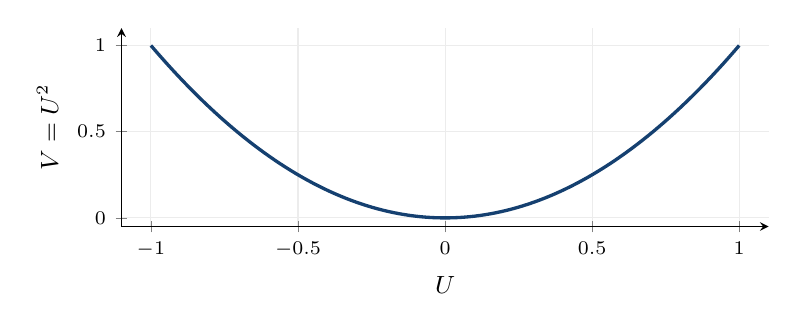
\begin{tikzpicture}
\begin{axis}[base,width=9.8cm,height=4.1cm,xmin=-1.1,xmax=1.1,ymin=-.05,ymax=1.1,xlabel={$U$},ylabel={$V=U^2$}]
\addplot[curva,domain=-1:1]{x*x};
\end{axis}
\end{tikzpicture}
\caption{La covarianza no detecta esta relación curva y simétrica.}
\end{figure}
\textbf{Independencia implica covarianza cero} cuando existen los momentos,
porque $\E[UV]=\E[U]\E[V]$. La implicación recíproca falla en el ejemplo.
Se recuperará para bloques de un vector \emph{conjuntamente} normal.
Normalidad marginal por separado no basta.

\topic{Condicionar: torre y descomposición de momentos}{s10}
Para una variable discreta $G$, observar $G=g$ cambia las probabilidades:
$\Prob(U=u\mid G=g)=\Prob(U=u,G=g)/\Prob(G=g)$.
La esperanza condicional es la función
\[
m(g)=\E[U\mid G=g]=\sum_u u\,\Prob(U=u\mid G=g).
\]
Antes de observar $G$, $m(G)$ es una variable aleatoria.
Para densidades se integra $u f_{U\mid G}(u\mid g)$.
En general se caracteriza por $\E[h(G)\{U-m(G)\}]=0$ para toda
función acotada $h$.

\textbf{Torre de expectativas.} Por suma de probabilidades conjuntas,
\[
\E[m(G)]
=\sum_g\sum_u u\,\Prob(U=u\mid G=g)\Prob(G=g)
=\sum_u u\,\Prob(U=u)=\E[U].
\]
Esta identidad incluye modelos continuos y mixtos.

\begin{teorema}[Ley de varianza total]
Si $\E[U^2]<\infty$,
\[
\boxed{\Var(U)=\E[\Var(U\mid G)]+\Var(\E[U\mid G])}.
\]
\end{teorema}
\begin{deduccion}
Descompongamos $U-\mu=(U-m(G))+(m(G)-\mu)$.
El término cruzado tiene esperanza cero:
\[
\E[(U-m(G))(m(G)-\mu)]
=\E[(m(G)-\mu)\E[U-m(G)\mid G]]=0.
\]
La esperanza del primer cuadrado es la media de las varianzas condicionales;
la del segundo es la varianza de la media condicional.
\end{deduccion}
Para dos variables, expandir el producto del mismo modo produce
\[
\boxed{\Cov(U,V)
=\E[\Cov(U,V\mid G)]
+\Cov(\E[U\mid G],\E[V\mid G])}.
\]
La variación dentro de grupos y la variación entre grupos son sumandos
diferentes; una covarianza agregada puede ser grande aun cuando sea cero
dentro de cada grupo.

\begin{ejemplo}[Mezcla de dos normales]
Sea $G\sim\operatorname{Bern}(1/2)$ y
$U\mid G=0\sim\Normal(0,1)$,
$U\mid G=1\sim\Normal(4,1)$.
Entonces $\E[U\mid G]=4G$ y $\Var(U\mid G)=1$:
\[
\E[U]=2,\quad \Var(U)=1+16\Var(G)=1+4=5.
\]
Si $V=2G+\eta$, donde $\eta$ es independiente de $(U,G)$ y tiene media
cero, $\Cov(U,V\mid G)=0$ pero
$\Cov(U,V)=\Cov(4G,2G)=8(1/4)=2$.
\end{ejemplo}
Para vectores, la misma expansión exterior da
\[
\Cov(x)=\E[\Cov(x\mid G)]+\Cov(\E[x\mid G]).
\]
Al estudiar un diseño aleatorio $X$, esta será la herramienta que conecta
la incertidumbre condicional de $\widehat\beta\mid X$ con su incertidumbre
sin condicionar. Nunca se debe omitir el segundo término sin comprobarlo.
\topic{Álgebra lineal: dimensiones, traza y productos}{s11}
Para $a,b\in\R^{p\times1}$, el producto interno y el exterior son distintos:
\[
a\T b=\sum_{j=1}^pa_jb_j\in\R,\qquad
ab\T=(a_ib_j)_{ij}\in\R^{p\times p}.
\]
Si $A\in\R^{q\times p}$, entonces $(Aa)_i=\sum_ja_{ij}^{(A)}a_j$ y
$Aa\in\R^q$. El número de columnas del primer factor debe coincidir con
el número de filas del segundo.

\textbf{La forma cuadrática.} Para $Q\in\R^{p\times p}$,
\[
a\T Qa=\sum_{i=1}^p\sum_{j=1}^pq_{ij}a_ia_j.
\]
Si $Q=Q\T$, los términos cruzados se agrupan:
\[
a\T Qa=\sum_iq_{ii}a_i^2+2\sum_{i<j}q_{ij}a_ia_j.
\]
Para $p=2$ y $Q=\begin{psmallmatrix}4&1\\1&9\end{psmallmatrix}$,
$a\T Qa=4a_1^2+2a_1a_2+9a_2^2$.
Esta expresión será la varianza de $a\T x$ cuando $Q=\Cov(x)$.

\textbf{Traza y normas.} La traza suma la diagonal:
$\tr(Q)=\sum_iq_{ii}$. Para $B\in\R^{m\times p}$,
\[
\norm B\F^2=\sum_{i,j}b_{ij}^2=\tr(B\T B),\qquad
\norm a_2^2=a\T a.
\]
Si $C\in\R^{p\times q}$ y $D\in\R^{q\times p}$,
\[
\tr(CD)=\sum_{i=1}^p\sum_{j=1}^qc_{ij}d_{ji}=\tr(DC).
\]
Por sucesivas rotaciones compatibles, $\tr(ABC)=\tr(BCA)=\tr(CAB)$.
No se concluye $\tr(ABC)=\tr(ACB)$.

\textbf{Rango, núcleo e inversa.} El rango es el número de columnas
linealmente independientes. El núcleo es
$\ker A=\{v:Av=0\}$. Para una matriz cuadrada $A$ de orden $p$,
\[
\rank(A)=p\ \Longleftrightarrow\ \ker A=\{0\}
\ \Longleftrightarrow\ A^{-1}\text{ existe}.
\]
Si $X\in\R^{n\times k}$,
$v\T X\T Xv=\norm{Xv}_2^2$. Por ello, $X\T X$ es invertible
exactamente cuando las columnas de $X$ son independientes.

\begin{ejemplo}[Producto exterior y suma de cuadrados]
Para $a=(2,-1,3)\T$,
\[
aa\T=\begin{pmatrix}4&-2&6\\-2&1&-3\\6&-3&9\end{pmatrix},
\qquad a\T a=14,\quad \tr(aa\T)=14,\quad \rank(aa\T)=1.
\]
Todos los vectores de la imagen de $aa\T$ son múltiplos de $a$:
$(aa\T)v=a(a\T v)$. Aunque hay nueve entradas, solo se genera una dirección.
\end{ejemplo}
\textbf{Pitágoras y proyección.}
Si $Q\in\R^{p\times r}$ tiene columnas ortonormales, $Q\T Q=I_r$.
La matriz $P=QQ\T$ cumple $P\T=P$ y $P^2=P$, y
\[
x=Px+(I-P)x,\quad
(Px)\T(I-P)x=0,\quad
\norm x_2^2=\norm{Px}_2^2+\norm{(I-P)x}_2^2.
\]
La igualdad permite separar variación explicada y residual.

\topic{Esperanza y covarianza vectorial}{s12}
Sea $x=(x_1,\ldots,x_p)\T$ con $\E[\norm x_2^2]<\infty$.
La esperanza se toma entrada por entrada:
\[
\mu=\E[x]=(\E[x_1],\ldots,\E[x_p])\T.
\]
Para una matriz aleatoria $B=(B_{ij})$, $\E[B]=(\E[B_{ij}])$.
Por tanto, la linealidad escalar demuestra la linealidad matricial.

\begin{definicion}[Covarianza entre dos vectores]
Para $x\in\R^p$ y $z\in\R^q$,
\[
\Cov(x,z)=\E[(x-\mu_x)(z-\mu_z)\T]
=\E[xz\T]-\mu_x\mu_z\T\in\R^{p\times q}.
\]
$\Cov(z,x)=\Cov(x,z)\T$. Escribimos $\Cov(x)=\Cov(x,x)$.
\end{definicion}
La entrada $(i,j)$ es $\Cov(x_i,z_j)$. En una autocovarianza,
la diagonal contiene varianzas y la matriz es simétrica. El segundo momento
$\E[xx\T]=\Sigma+\mu\mu\T$ no es la covarianza salvo si $\mu=0$.

\begin{teorema}[Transformación afín]
Para matrices fijas $A\in\R^{r\times p}$, $B\in\R^{s\times q}$ y
vectores constantes $a,b$,
\[
\E[Ax+a]=A\mu_x+a,\quad
\boxed{\Cov(Ax+a,Bz+b)=A\Cov(x,z)B\T}.
\]
\end{teorema}
\begin{deduccion}
Los vectores centrados son $A(x-\mu_x)$ y $B(z-\mu_z)$.
Su producto exterior es
$A(x-\mu_x)(z-\mu_z)\T B\T$.
Como $A,B$ son fijas, se sacan de la esperanza conservando su orden.
Las dimensiones finales son $(r\times p)(p\times q)(q\times s)=r\times s$.
\end{deduccion}
Para una combinación escalar $L=c\T x$, esta identidad se reduce a
\[
\boxed{\Var(L)=c\T\Sigma c},\qquad
\Cov(c\T x,d\T x)=c\T\Sigma d.
\]
Así, la covarianza es una forma bilineal, y la varianza una forma cuadrática.

\begin{ejemplo}[Dos transformaciones simultáneas]
Con $\mu=(1,2)\T$,
$\Sigma=\begin{psmallmatrix}4&1\\1&9\end{psmallmatrix}$,
$A=\begin{psmallmatrix}1&1\\1&-1\end{psmallmatrix}$ y $a=(3,0)\T$,
\[
A\Sigma=\begin{pmatrix}5&10\\3&-8\end{pmatrix},\qquad
A\Sigma A\T=\begin{pmatrix}15&-5\\-5&11\end{pmatrix},
\qquad \E[Ax+a]=(6,-1)\T.
\]
$\Var(x_1+x_2)=15$, $\Var(x_1-x_2)=11$ y su covarianza es $-5$.
\end{ejemplo}
Si $v=(x\T,z\T)\T$, la matriz conjunta tiene bloques
\[
\Cov(v)=
\begin{pmatrix}\Sigma_x&\Sigma_{xz}\\\Sigma_{xz}\T&\Sigma_z\end{pmatrix}.
\]
Para sumas de vectores de la misma dimensión,
$\Cov(x+z)=\Sigma_x+\Sigma_z+\Sigma_{xz}+\Sigma_{xz}\T$.
Una covarianza cruzada no tiene por qué ser cuadrada ni simétrica.

\topic{Positividad, rango y direcciones deterministas}{s13}
La matriz $\Sigma=\Cov(x)$ tiene una propiedad más fuerte que la simetría.
Para cualquier $a\in\R^p$,
\[
a\T\Sigma a
=\E[a\T(x-\mu)(x-\mu)\T a]
=\E[\{a\T(x-\mu)\}^2]\ge0.
\]
Una matriz simétrica que cumple esto es \textbf{semidefinida positiva},
$\Sigma\succeq0$. Es \textbf{definida positiva}, $\Sigma\succ0$, si la
desigualdad es estricta para todo $a\ne0$.

\textbf{Qué significa ser singular.}
Si $a\T\Sigma a=0$ para algún $a\ne0$, entonces
$a\T(x-\mu)=0$ casi seguramente.
Todos los resultados viven en el hiperplano afín $a\T x=a\T\mu$.
También $\Sigma a=0$: entrada por entrada,
$\E[(x_i-\mu_i)a\T(x-\mu)]=0$.
Por tanto,
\[
\ker\Sigma=\{a:a\T(x-\mu)=0\text{ casi seguramente}\}.
\]
La singularidad no implica que una variable individual sea constante;
puede reflejar una combinación exacta.

\begin{ejemplo}[Dos coordenadas, una única fuente]
Sea $U$ de media cero y varianza uno, y $x=(U,2U)\T$. Entonces
\[
\Sigma=\begin{pmatrix}1&2\\2&4\end{pmatrix},\quad
\det\Sigma=0,\quad
\Sigma(-2,1)\T=0.
\]
Ambas varianzas son positivas, pero $x_2-2x_1=0$.
Los autovalores son $5$ y $0$; solo una dirección tiene dispersión.
\end{ejemplo}

\textbf{Restricciones a las entradas.} Para dos coordenadas, el teorema
Cauchy--Schwarz exige
\[
\Sigma_{ij}^2\le\Sigma_{ii}\Sigma_{jj}.
\]
Así, $\begin{psmallmatrix}1&2\\2&1\end{psmallmatrix}$ no puede ser una
covarianza: el vector $(1,-1)\T$ produce una forma cuadrática $-2$.
No toda matriz simétrica es una matriz de covarianza.

\textbf{Cualquier matriz positiva puede construirse.}
Cuando $\Sigma=Q\Lambda Q\T$ con $Q$ ortogonal y
$\Lambda=\diag(\lambda_1,\ldots,\lambda_p)$, $\lambda_j\ge0$, definimos
$L=Q\Lambda^{1/2}$. Si $z$ tiene media cero y covarianza $I_p$, entonces
\[
x=\mu+Lz,\qquad
\E[x]=\mu,\quad \Cov(x)=LL\T=Q\Lambda Q\T=\Sigma.
\]
No se necesita que $z$ sea normal para construir los momentos. Si lo es,
la misma construcción define una normal multivariada.

\begin{idea}[Dispersión total y dispersión direccional]
$\tr(\Sigma)=\sum_j\Var(x_j)=\E[\norm{x-\mu}_2^2]$ es la dispersión
cuadrática total. Para una dirección unitaria $a$, $a\T\Sigma a$ es
la varianza de la coordenada proyectada. El determinante, cuando es
positivo, mide un producto de dispersiones principales y cambia con las
unidades: no sustituye a la traza.
\end{idea}


\begin{figure}[H]\centering
\tdplotsetmaincoords{65}{115}
\begin{tikzpicture}[tdplot_main_coords,scale=1.02]
\draw[eje](-2.7,0,0)--(2.7,0,0)node[right]{$x_1$};
\draw[eje](0,-1.5,0)--(0,1.6,0)node[right]{$x_2$};
\draw[eje](0,0,-.8)--(0,0,1)node[above]{$x_3$};
\foreach \a in {-60,-30,0,30,60}{
\draw[azul!65,thick]plot[domain=0:360,samples=80,variable=\t]({2*cos(\a)*cos(\t)},{cos(\a)*sin(\t)},{.5*sin(\a)});
}
\foreach \a in {0,30,60,90,120,150}{
\draw[azul!65,thick]plot[domain=0:360,samples=80,variable=\t]({2*cos(\a)*cos(\t)},{sin(\a)*cos(\t)},{.5*sin(\t)});
}
\end{tikzpicture}
\caption{Elipsoide de $\Sigma=\diag(4,1,1/4)$: semiejes $2,1,1/2$. Un autovalor cero aplana una dirección.}
\end{figure}
\topic{Ejemplo de tres variables con factores comunes}{s14}
Sean $U,V,W$ independientes, centrados y de varianza uno. No requerimos
normalidad. Construimos
\[
x_1=1+U,\qquad x_2=2+2U+V,\qquad
x_3=-1+U+V+W.
\]
En forma matricial,
\[
x=\mu+Az,\quad
\mu=\begin{pmatrix}1\\2\\-1\end{pmatrix},\quad
z=\begin{pmatrix}U\\V\\W\end{pmatrix},\quad
A=\begin{pmatrix}1&0&0\\2&1&0\\1&1&1\end{pmatrix}.
\]
Como $\Cov(z)=I_3$, $\Sigma=AA\T$. Multiplicando filas entre sí:
\[
\Sigma=
\begin{pmatrix}
1^2&1\cdot2&1\cdot1\\
2\cdot1&2^2+1^2&2\cdot1+1\cdot1\\
1\cdot1&1\cdot2+1\cdot1&1^2+1^2+1^2
\end{pmatrix}
=\begin{pmatrix}1&2&1\\2&5&3\\1&3&3\end{pmatrix}.
\]
Cada covarianza nace de factores que comparten las dos variables.
Por ejemplo, $\Cov(x_2,x_3)=2\Var(U)+\Var(V)=3$.

\textbf{Segundo momento completo.} El producto de medias es
\[
\mu\mu\T=\begin{pmatrix}1&2&-1\\2&4&-2\\-1&-2&1\end{pmatrix},
\quad
\E[xx\T]=\begin{pmatrix}2&4&0\\4&9&1\\0&1&4\end{pmatrix}.
\]
Aquí $\E[x_1x_3]=0$, pero $\Cov(x_1,x_3)=1$ porque las medias no son cero.

\begin{ejemplo}[Una combinación con términos positivos y negativos]
Para $c=(1,-1,2)\T$, $L=c\T x=x_1-x_2+2x_3$ tiene
\[
\E[L]=1-2+2(-1)=-3,\quad
A\T c=(1,1,2)\T.
\]
Luego $L=-3+U+V+2W$ y $\Var(L)=1+1+4=6$. Por la matriz,
\[
\Sigma c=(1,3,4)\T,\qquad c\T\Sigma c=1-3+8=6.
\]
La expansión escalar produce lo mismo:
$1+5+4(3)+2(-2+2-6)=6$.
\end{ejemplo}
Para $d=(0,1,-1)\T$, $M=d\T x$ tiene
$\E[M]=3$, $A\T d=(1,0,-1)\T$ y $\Var(M)=2$.
La covarianza entre ambas combinaciones es
\[
\Cov(L,M)=c\T\Sigma d=(A\T c)\T(A\T d)=1-2=-1.
\]
El vector $(L,M)\T$ tiene, por tanto,
\[
\E\begin{pmatrix}L\\M\end{pmatrix}
=\begin{pmatrix}-3\\3\end{pmatrix},\qquad
\Cov\begin{pmatrix}L\\M\end{pmatrix}
=\begin{pmatrix}6&-1\\-1&2\end{pmatrix}.
\]
\textbf{Recuperar factores.} Como $\det A=1$, $A$ es invertible:
\[
U=x_1-1,\quad
V=x_2-2x_1,\quad
W=x_3-x_2+x_1+2.
\]
Estas coordenadas tienen covarianza identidad.
La matriz original contiene nueve entradas, pero las tres fórmulas
revelan cómo se genera su dependencia. En dimensión $p$, el mismo
procedimiento usa una factorización $\Sigma=LL\T$.

\topic{Cálculo vectorial: gradiente, Hessiana y Taylor}{s15}
Sea $f:\R^k\to\R$ diferenciable, con argumento columna $\theta$.
El gradiente es $\nabla_\theta f=(\partial f/\partial\theta_j)_{j=1}^k$,
y el diferencial es $\dd f=(\nabla f)\T\dd\theta$.
La Hessiana contiene segundas derivadas:
$H_{ij}=\partial^2f/(\partial\theta_i\partial\theta_j)$.

\textbf{Derivar un producto cuadrático sin reglas ocultas.}
Para $f(\theta)=\theta\T A\theta=\sum_{i,j}a_{ij}\theta_i\theta_j$,
\[
\frac{\partial f}{\partial\theta_\ell}
=\sum_ja_{\ell j}\theta_j+\sum_i a_{i\ell}\theta_i,
\quad
\boxed{\nabla f=(A+A\T)\theta}.
\]
Si $A$ es simétrica, $\nabla f=2A\theta$ y $H=2A$.
Para $f(\theta)=b\T\theta$, $\nabla f=b$ y $H=0$.

\textbf{Mínimos cuadrados.} Con $y\in\R^n$ y $X\in\R^{n\times k}$,
\[
f(\theta)=\norm{y-X\theta}_2^2
=y\T y-2\theta\T X\T y+\theta\T X\T X\theta,
\]
\[
\nabla f=-2X\T y+2X\T X\theta,\qquad H=2X\T X.
\]
La Hessiana es semidefinida positiva, porque
$v\T Hv=2\norm{Xv}_2^2\ge0$. Si $X$ tiene rango $k$,
es definida positiva y el mínimo es único.

\textbf{Taylor multivariado.} Para un incremento pequeño $h$ y $f$ dos
veces diferenciable,
\[
f(\theta+h)=f(\theta)+(\nabla f(\theta))\T h
+\tfrac12h\T H(\theta)h+o(\norm h_2^2).
\]
Para $g:\R^k\to\R^q$, el Jacobiano
$J_g=(\partial g_i/\partial\theta_j)\in\R^{q\times k}$ permite escribir
$g(\theta+h)=g(\theta)+J_gh+o(\norm h_2)$.
Al transformar estimadores, esto da la covarianza aproximada $J_gVJ_g\T$.

\begin{ejemplo}[Un cociente de dos coeficientes]
$g(\theta)=\theta_1/\theta_2$, $\theta_2\ne0$:
\[
J_g=\begin{pmatrix}1/\theta_2&-\theta_1/\theta_2^2\end{pmatrix}.
\]
Si $V=\Cov(\widehat\theta)$ y el estimador está cerca de $\theta$,
\[
\Var(g(\widehat\theta))\approx
\frac{V_{11}}{\theta_2^2}
+\frac{\theta_1^2V_{22}}{\theta_2^4}
-\frac{2\theta_1V_{12}}{\theta_2^3}.
\]
Cuando el denominador se acerca a cero, la aproximación puede ser inadecuada.
\end{ejemplo}
\textbf{Regla de la cadena.}
$\nabla_\theta f(g(\theta))=J_g(\theta)\T\nabla_g f$.
Por dimensiones, $(k\times q)(q\times1)=k\times1$.
En una restricción $c(\theta)=0$, el lagrangiano
$\mathcal L=f(\theta)-\lambda c(\theta)$ exige
$\nabla f=\lambda\nabla c$ y $c=0$. Para $c=\theta\T\theta-1$,
$\nabla c=2\theta$: esta igualdad llevará directamente a PCA.

\begin{figure}[H]\centering
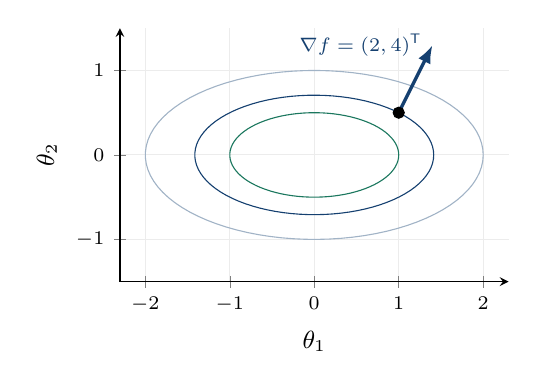
\begin{tikzpicture}
\begin{axis}[base,width=10cm,height=4.8cm,axis equal image,xmin=-2.3,xmax=2.3,ymin=-1.5,ymax=1.5,xlabel={$\theta_1$},ylabel={$\theta_2$}]
\addplot[azul!40,domain=0:360,variable=\t,samples=90]({2*cos(t)},{sin(t)});
\addplot[azul,domain=0:360,variable=\t,samples=90]({sqrt(2)*cos(t)},{sin(t)/sqrt(2)});
\addplot[verde,domain=0:360,variable=\t,samples=90]({cos(t)},{sin(t)/2});
\draw[vec] (axis cs:1,.5)--(axis cs:1.4,1.3)node[left,font=\scriptsize]{$\nabla f=(2,4)^\mathsf T$};
\addplot[only marks,mark=*]coordinates{(1,.5)};
\end{axis}
\end{tikzpicture}
\caption{$f(\theta)=\theta_1^2+4\theta_2^2$: el gradiente es perpendicular al nivel y señala mayor crecimiento.}
\end{figure}
\topic{Diferenciales matriciales, inversa y determinante}{s16}
Para una matriz variable $A\in\R^{p\times p}$, $\dd A$ agrupa incrementos
de sus entradas. El diferencial conserva el orden de los productos:
\[
\dd(AB)=(\dd A)B+A(\dd B),\qquad
\dd(A\T)=(\dd A)\T,\qquad
\dd\tr(A)=\tr(\dd A).
\]
El gradiente matricial de $f$ se define mediante
$\dd f=\tr((\nabla_Af)\T\dd A)$.

\textbf{Inversa.} Diferenciando $AA^{-1}=I$,
\[
(\dd A)A^{-1}+A\,\dd(A^{-1})=0
\quad\Longrightarrow\quad
\boxed{\dd(A^{-1})=-A^{-1}(\dd A)A^{-1}}.
\]
Si $A(t)$ depende de un escalar,
$\frac{\dd}{\dd t}A(t)^{-1}=-A(t)^{-1}A'(t)A(t)^{-1}$.
El producto no puede reemplazarse por $-A'/A^2$ salvo en el caso escalar
o bajo conmutatividad pertinente.

\textbf{Determinante.} Para $A$ invertible,
$\det(A+\dd A)=\det A\det(I+A^{-1}\dd A)$.
En el determinante de $I+B$, los términos lineales son las entradas
diagonales de $B$; los restantes tienen orden al menos dos:
\[
\det(I+B)=1+\tr(B)+O(\norm B^2).
\]
Por ello,
\[
\dd\det A=\det A\,\tr(A^{-1}\dd A),\qquad
\boxed{\dd\log\det A=\tr(A^{-1}\dd A)}
\]
cuando $\det A>0$, en particular si $A\succ0$.

\textbf{Dos derivadas que aparecen en la normal.}
Con $r$ fijo y $A\succ0$,
\[
\dd(r\T A^{-1}r)
=-r\T A^{-1}(\dd A)A^{-1}r
=-\tr(A^{-1}rr\T A^{-1}\dd A).
\]
Con $B\in\R^{k\times q}$ variable,
\[
f(B)=\norm{Y-XB}\F^2,\qquad
\dd f=-2\tr\{(Y-XB)\T X\dd B\},
\quad \nabla_Bf=-2X\T(Y-XB).
\]

\begin{ejemplo}[Comprobar la inversa en un caso diagonal]
$A(t)=\diag(1+t,2+t)$ tiene
$A'(t)=I_2$ y
\[
\frac{\dd}{\dd t}A(t)^{-1}
=-\diag((1+t)^{-2},(2+t)^{-2}).
\]
Asimismo,
$\frac{\dd}{\dd t}\log\det A(t)
=(1+t)^{-1}+(2+t)^{-1}=\tr(A(t)^{-1})$.
\end{ejemplo}
\textbf{Segunda variación.} Para una dirección simétrica $H$,
\[
\frac{\dd^2}{\dd t^2}\log\det(A+tH)\bigg|_{t=0}
=-\tr(A^{-1}HA^{-1}H)\le0.
\]
La desigualdad se obtiene al escribir la traza como
$\tr\{(A^{-1/2}HA^{-1/2})^2\}$, suma de cuadrados de autovalores.
Así, $\log\det$ es cóncava sobre matrices definidas positivas.
La derivada se toma dentro del dominio donde $A+tH\succ0$.

\topic{Proyección en L2 y mejor predicción lineal}{s17}
El espacio $L^2$ contiene variables con segundo momento finito. El producto
interno y su norma son
$\ip UV=\E[UV]$ y $\norm U_{L^2}^2=\E[U^2]$.
Para variables centradas, $\ip UV=\Cov(U,V)$.
Una proyección minimiza la norma del error y vuelve ortogonal ese error
al espacio de predictores.

\textbf{Predicción lineal de un escalar.}
Sean $Y$ una respuesta y $x\in\R^p$, con $\Sigma_x\succ0$.
Buscamos minimizar $\E[(Y-a-b\T x)^2]$.
Para $b$ fijo, la media del residuo debe ser cero:
$a=\mu_Y-b\T\mu_x$.
Centrando $Y_c=Y-\mu_Y$ y $x_c=x-\mu_x$,
\[
Q(b)=\E[(Y_c-b\T x_c)^2]
=\Var(Y)-2b\T\Sigma_{xY}+b\T\Sigma_x b.
\]
El gradiente $-2\Sigma_{xY}+2\Sigma_xb$ se anula en
\[
\boxed{b_*=\Sigma_x^{-1}\Sigma_{xY},\qquad
a_*=\mu_Y-b_*\T\mu_x}.
\]
Para $e=Y_c-b_*\T x_c$,
\[
\E[e]=0,\quad \Cov(x,e)=\Sigma_{xY}-\Sigma_xb_*=0,
\quad
\Var(e)=\Var(Y)-\Sigma_{Yx}\Sigma_x^{-1}\Sigma_{xY}.
\]
Además, $Q(b)=Q(b_*)+(b-b_*)\T\Sigma_x(b-b_*)$ demuestra que el
mínimo es global y único.

\begin{ejemplo}[Predecir con un predictor]
Si $\Var(x)=4$, $\Var(Y)=9$ y $\Cov(x,Y)=3$, entonces
$b_*=3/4$, $\Var(e)=9-9/4=27/4$.
Con medias cero, la varianza de $\widehat Y=(3/4)x$ es $9/4$:
$9=9/4+27/4$. El término cruzado es cero por ortogonalidad.
\end{ejemplo}
\textbf{La mejor predicción entre todas las funciones.}
Sea $m(x)=\E[Y\mid x]$. Para cualquier función $g$ de segundo momento
finito, expandir y condicionar da
\[
\E[(Y-g(x))^2]
=\E[(Y-m(x))^2]+\E[(m(x)-g(x))^2].
\]
El término cruzado desaparece porque $\E[Y-m(x)\mid x]=0$.
Por tanto, $m(x)$ es la mejor predicción cuadrática entre todas las
funciones de $x$; $a_*+b_*\T x$ es la mejor entre las funciones afines.

\begin{cuidado}[Ortogonalidad y media condicional cero]
$\Cov(x,e)=0$ solo impone $p$ momentos. $\E[e\mid x]=0$ implica
ortogonalidad respecto de toda función integrable de $x$.
Si $Y=x^2$ con $x$ uniforme y simétrico, la mejor recta es constante,
pero la media condicional verdadera es $x^2$.
\end{cuidado}
La normal multivariada volverá afín esa media condicional. MCO estimará
las ecuaciones normales usando momentos muestrales. IV cambiará
las variables respecto de las cuales se exige ortogonalidad.


\begin{figure}[H]\centering
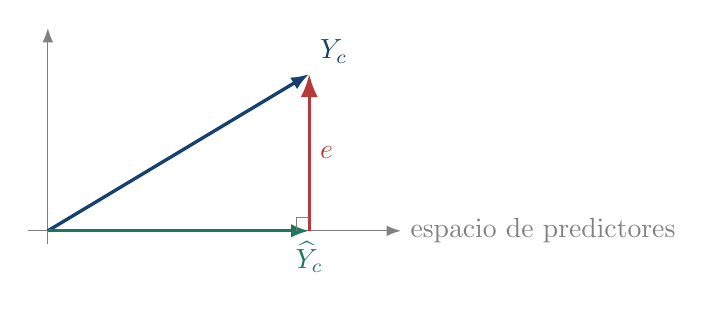
\begin{tikzpicture}[scale=.83]
\draw[eje](-.3,0)--(5.4,0)node[right]{espacio de predictores};
\draw[eje](0,-.2)--(0,3.1);
\draw[vec](0,0)--(4,2.4)node[above right]{$Y_c$};
\draw[vverde](0,0)--(4,0)node[below]{$\widehat Y_c$};
\draw[rojo,very thick,-{Latex}](4,0)--(4,2.4)node[midway,right]{$e$};
\draw[gray](3.8,0)--(3.8,.2)--(4,.2);
\end{tikzpicture}
\caption{Geometría de $L^2$: $\E[Y_c^2]=\E[\widehat Y_c^2]+\E[e^2]$ porque $\E[\widehat Y_c e]=0$.}
\end{figure}
\topic{Matrices aleatorias, vectorización y Kronecker}{s18}
Una matriz aleatoria $B\in\R^{m\times p}$ tiene $mp$ coordenadas.
Para conservar \emph{todas} sus covarianzas, apilamos columnas:
\[
\vecop(B)=(B_{11},\ldots,B_{m1},B_{12},\ldots,B_{mp})\T\in\R^{mp}.
\]
$\Cov(\vecop B)$ tiene tamaño $mp\times mp$, y la covarianza entre
$B_{ij}$ y $B_{rs}$ ocupa las posiciones $i+m(j-1)$ y $r+m(s-1)$.
El producto $\E[(B-\E B)(B-\E B)\T]$, de tamaño $m\times m$,
suma sobre columnas y no contiene toda esa información.

\textbf{Producto de Kronecker.}
Si $A=(a_{ij})\in\R^{r\times s}$ y $C\in\R^{m\times p}$,
\[
A\otimes C=
\begin{pmatrix}a_{11}C&\cdots&a_{1s}C\\
\vdots&\ddots&\vdots\\a_{r1}C&\cdots&a_{rs}C\end{pmatrix}
\in\R^{rm\times sp}.
\]
Para $LBR$ con dimensiones compatibles,
\[
\boxed{\vecop(LBR)=(R\T\otimes L)\vecop(B)}.
\]
En la entrada $(i,j)$, ambos lados suman
$\sum_{a,b}L_{ia}B_{ab}R_{bj}$, lo que prueba la identidad.

\textbf{Normal matricial.}
Escribimos $B\sim\mathcal{MN}_{m,p}(M,U,V)$ si
\[
\vecop(B)\sim\Normal_{mp}(\vecop M,V\otimes U).
\]
$U\in\R^{m\times m}$ controla filas y $V\in\R^{p\times p}$ columnas:
\[
\Cov(B_{ij},B_{rs})=U_{ir}V_{js}.
\]
Puede construirse como $B=M+L_U G L_V\T$, donde $G$ tiene entradas
iid normales estándar y $L_UL_U\T=U$, $L_VL_V\T=V$.
Vectorizar y aplicar la transformación de covarianzas prueba la fórmula.

\begin{ejemplo}[Cuatro entradas y dieciséis covarianzas]
Con $U=\begin{psmallmatrix}1&.5\\.5&2\end{psmallmatrix}$,
$V=\begin{psmallmatrix}4&1\\1&3\end{psmallmatrix}$,
\[
V\otimes U=
\begin{pmatrix}
4&2&1&.5\\2&8&.5&2\\1&.5&3&1.5\\.5&2&1.5&6
\end{pmatrix}.
\]
El orden es $(B_{11},B_{21},B_{12},B_{22})$.
En particular, $\Var(B_{21})=8$ y $\Cov(B_{11},B_{22})=.5$.
\end{ejemplo}
Para transformaciones fijas,
\[
LBR\sim\mathcal{MN}(LMR,LUL\T,R\T VR).
\]
Además, en una normal matricial centrada,
$\E[BB\T]=\tr(V)U$ y $\E[B\T B]=\tr(U)V$;
se comprueban sumando las covarianzas de cada producto de entradas.
La representación Kronecker impone una estructura separable:
una covarianza arbitraria de tamaño $mp\times mp$ no tiene que factorizar así.

\topic{Construcción y densidad de la normal multivariada}{s19}
Sea $z=(z_1,\ldots,z_p)\T$ con entradas independientes
$\Normal(0,1)$. Su densidad conjunta es el producto:
\[
f_z(z)=(2\pi)^{-p/2}\exp(-z\T z/2),\quad
\E[z]=0,\quad \Cov(z)=I_p.
\]
Para $L\in\R^{p\times p}$ invertible y $\mu\in\R^p$, sea $x=\mu+Lz$.
Entonces $\E[x]=\mu$ y $\Sigma=LL\T\succ0$.
El cambio $z=L^{-1}(x-\mu)$ tiene Jacobiano
$\abs{\det L}^{-1}=(\det\Sigma)^{-1/2}$:
\[
\boxed{
f_x(x)=\frac{\exp\{-\tfrac12(x-\mu)\T\Sigma^{-1}(x-\mu)\}}
{(2\pi)^{p/2}(\det\Sigma)^{1/2}}
}.
\]
Esta distribución se denota $\Normal_p(\mu,\Sigma)$ \cite{mitnormal}.
La igualdad
$z\T z=(x-\mu)\T L^{-\mathsf T}L^{-1}(x-\mu)$ demuestra el exponente.

\textbf{Por qué la construcción no depende de la raíz elegida.}
Su función característica es
\[
\varphi_x(t)=\E[e^{\,\mathrm i t\T x}]
=\exp(\mathrm i t\T\mu-\tfrac12t\T\Sigma t).
\]
Se obtiene multiplicando las características normales de las coordenadas
de $z$. Solo depende de $\mu,\Sigma$, que identifican la distribución normal.
La función generadora real es
$M_x(t)=\exp(t\T\mu+\tfrac12t\T\Sigma t)$.

\textbf{Todas las combinaciones son normales.}
Para $a\in\R^p$,
\[
a\T x\sim\Normal(a\T\mu,a\T\Sigma a).
\]
Para $A\in\R^{q\times p}$,
$Ax+b\sim\Normal_q(A\mu+b,A\Sigma A\T)$.
Si la covarianza resultante es singular, se interpreta como normal
degenerada, no mediante una densidad ordinaria en todo $\R^q$.

\begin{ejemplo}[Generar correlación a partir de independencia]
Para normales estándar independientes $Z_1,Z_2$,
\[
x_1=Z_1,\quad x_2=\rho Z_1+\sqrt{1-\rho^2}\,Z_2,\quad \abs\rho<1,
\]
\[
\mu=0,\quad \Sigma=\begin{pmatrix}1&\rho\\\rho&1\end{pmatrix}.
\]
La densidad es
$\exp\{-(x_1^2-2\rho x_1x_2+x_2^2)/[2(1-\rho^2)]\}
/[2\pi\sqrt{1-\rho^2}]$.
Para $\rho=1$, $x_2=x_1$ y la distribución vive en una recta.
\end{ejemplo}
\textbf{Independencia de bloques gaussianos.}
Si $x=(a\T,b\T)\T$ es conjuntamente normal y $\Cov(a,b)=0$,
la función característica conjunta factoriza en las dos marginales.
Por unicidad de la función característica, $a$ y $b$ son independientes.
Aquí la normalidad conjunta es la hipótesis que convierte
ortogonalidad en independencia.
Una colección de marginales normales con dependencia no gaussiana no
satisface necesariamente este resultado.


\begin{figure}[H]\centering
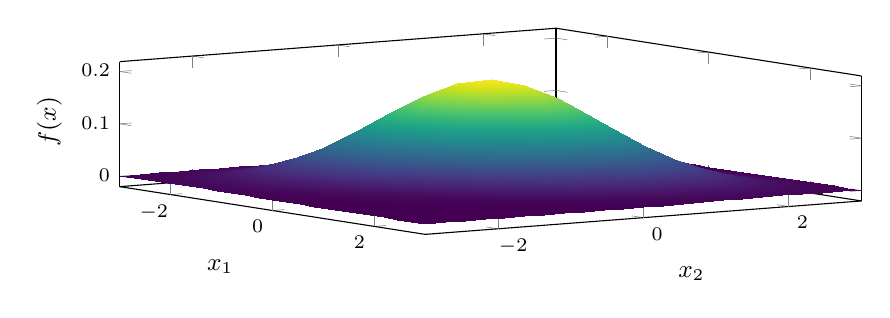
\begin{tikzpicture}
\begin{axis}[width=11cm,height=4.2cm,view={55}{25},xlabel={$x_1$},ylabel={$x_2$},zlabel={$f(x)$},tick label style={font=\scriptsize},label style={font=\small},colormap/viridis]
\addplot3[surf,shader=interp,domain=-3:3,y domain=-3:3,samples=23,samples y=23]{exp(-(x*x-1.2*x*y+y*y)/1.28)/(1.6*pi)};
\end{axis}
\end{tikzpicture}
\caption{Densidad $\Normal_2(0,\Sigma)$ con varianzas uno y correlación $.6$: la dependencia inclina la superficie.}
\end{figure}
\topic{Momentos gaussianos y formas cuadráticas}{s20}
Para $x\sim\Normal_p(0,\Sigma)$, derivar
$M_x(t)=\exp(\tfrac12t\T\Sigma t)$ en cero produce
$\E[x_ix_j]=\Sigma_{ij}$ y momentos impares nulos.
Para el cuarto orden,
\[
\boxed{\E[x_ix_jx_rx_s]
=\Sigma_{ij}\Sigma_{rs}+\Sigma_{ir}\Sigma_{js}
+\Sigma_{is}\Sigma_{jr}}.
\]
En la expansión $M_x(t)=1+\tfrac12t\T\Sigma t+
\tfrac18(t\T\Sigma t)^2+\cdots$, solo el término cuadrático en
$t\T\Sigma t$ contribuye al cuarto orden. Las tres maneras de emparejar
cuatro índices originan los tres productos. Índices repetidos siguen
la misma regla: $\E[x_i^4]=3\Sigma_{ii}^2$.

\textbf{Media de una forma cuadrática, sin normalidad.}
Para $A=A\T$ fijo y $x$ de media $\mu$,
\[
\E[x\T Ax]=\E[\tr(Axx\T)]
=\tr(A\E[xx\T])
=\boxed{\tr(A\Sigma)+\mu\T A\mu}.
\]
Para normales centradas, la fórmula de cuarto orden permite calcular
la varianza y la covarianza entre formas:
\[
\boxed{\Var(x\T Ax)=2\tr(A\Sigma A\Sigma)},\qquad
\boxed{\Cov(x\T Ax,x\T Bx)=2\tr(A\Sigma B\Sigma)}
\]
con $A,B$ simétricas.
Para comprobarlo, expandimos
$\sum_{i,j,r,s}a_{ij}b_{rs}\E[x_ix_jx_rx_s]$.
El primer emparejamiento cancela el producto de medias;
los otros dos dan la misma traza por simetría.

\textbf{Normal con media no nula.} Escribiendo $x=\mu+z$,
\[
x\T Ax=\mu\T A\mu+2\mu\T Az+z\T Az.
\]
El término lineal y el cuadrático centrado tienen covarianza cero porque
los momentos de tercer orden de $z$ son nulos. Por ello,
\[
\Var(x\T Ax)=2\tr(A\Sigma A\Sigma)+4\mu\T A\Sigma A\mu.
\]
Una covarianza cero entre estos dos términos no garantiza independencia
en este caso, pues el término cuadrático no es normal.

\begin{ejemplo}[Suma de cuadrados y proyecciones]
Para $z\sim\Normal_n(0,I_n)$ y una proyección ortogonal $P$ de rango $r$,
\[
\E[z\T Pz]=\tr P=r,\quad
\Var(z\T Pz)=2\tr(P^2)=2r.
\]
Una rotación ortogonal diagonaliza $P$ en $r$ unos y $n-r$ ceros:
$z\T Pz$ es suma de $r$ normales estándar al cuadrado, luego es
$\chi^2_r$.
\end{ejemplo}
Para una $A$ simétrica general,
$z\T Az=\sum_j\lambda_j\xi_j^2$ con $\xi_j$ iid normales estándar.
No es necesariamente chi-cuadrado: requiere los pesos adecuados.
La derivación explica por qué los grados de libertad de los residuos
de MCO serán el rango de una matriz de proyección.

\begin{figure}[H]\centering
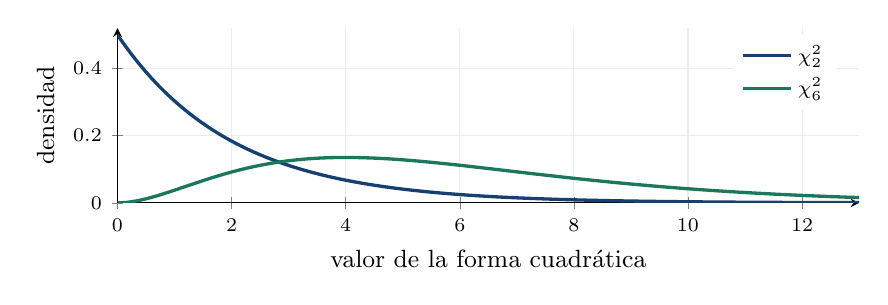
\begin{tikzpicture}
\begin{axis}[base,width=11cm,height=3.8cm,xmin=0,xmax=13,ymin=0,ymax=.52,xlabel={valor de la forma cuadrática},ylabel={densidad},legend pos=north east]
\addplot[curva,domain=0:13]{.5*exp(-x/2)};\addlegendentry{$\chi^2_2$}
\addplot[verde,very thick,domain=0:13]{x*x*exp(-x/2)/16};\addlegendentry{$\chi^2_6$}
\end{axis}
\end{tikzpicture}
\caption{Sumar cuadrados de más direcciones cambia la distribución y los dos primeros momentos.}
\end{figure}
\topic{Normal condicional y complemento de Schur}{s21}
Particionemos una normal conjunta:
\[
\begin{pmatrix}a\\b\end{pmatrix}
\sim\Normal_{r+s}\!\left(
\begin{pmatrix}\mu_a\\\mu_b\end{pmatrix},
\begin{pmatrix}\Sigma_{aa}&\Sigma_{ab}\\
\Sigma_{ba}&\Sigma_{bb}\end{pmatrix}\right),
\quad \Sigma_{bb}\succ0.
\]
Definimos $C=\Sigma_{ab}\Sigma_{bb}^{-1}$ y
$e=a-\mu_a-C(b-\mu_b)$. Por las reglas afines,
\[
\E[e]=0,\qquad
\Cov(e,b)=\Sigma_{ab}-C\Sigma_{bb}=0.
\]
Como $(e,b)$ es conjuntamente normal, $e$ y $b$ son independientes.
Además, expandir los cuatro términos de la covarianza da
\[
\Cov(e)=\Sigma_{aa}-C\Sigma_{ba}-\Sigma_{ab}C\T
+C\Sigma_{bb}C\T
=\Sigma_{aa}-\Sigma_{ab}\Sigma_{bb}^{-1}\Sigma_{ba}.
\]
Por tanto, al fijar $b$,
\[
\boxed{
a\mid b\sim\Normal_r\!\left(
\mu_a+\Sigma_{ab}\Sigma_{bb}^{-1}(b-\mu_b),
\ \Sigma_{aa}-\Sigma_{ab}\Sigma_{bb}^{-1}\Sigma_{ba}
\right)}.
\]
La covarianza condicional no depende del valor observado de $b$ en este
modelo. La media condicional sí lo hace.

\textbf{Complemento de Schur.} La matriz
$S_a=\Sigma_{aa}-\Sigma_{ab}\Sigma_{bb}^{-1}\Sigma_{ba}$
es positiva semidefinida porque es una covarianza.
Otra prueba completa cuadrados:
\[
\begin{pmatrix}v\\w\end{pmatrix}\T\Sigma
\begin{pmatrix}v\\w\end{pmatrix}
=v\T S_av+
(w+\Sigma_{bb}^{-1}\Sigma_{ba}v)\T
\Sigma_{bb}(w+\Sigma_{bb}^{-1}\Sigma_{ba}v).
\]
Si $\Sigma\succ0$, también $S_a\succ0$. Esta descomposición permite
derivar el determinante
$\det\Sigma=\det\Sigma_{bb}\det S_a$ y las fórmulas de inversa por bloques.

\begin{ejemplo}[Condicionar dos normales correlacionadas]
Con $\mu=(1,2)\T$ y
$\Sigma=\begin{psmallmatrix}4&3\\3&9\end{psmallmatrix}$,
\[
x_1\mid x_2=t\sim\Normal\!\left(
1+\tfrac13(t-2),\ 4-\tfrac{3^2}{9}
\right)=\Normal(1+(t-2)/3,3).
\]
Si $t=5$, la media condicional es $2$ y la varianza $3$.
La varianza total se recupera:
$\E[\Var(x_1\mid x_2)]+\Var(\E[x_1\mid x_2])
=3+(1/3)^2\cdot9=4$.
\end{ejemplo}
\textbf{Reducir incertidumbre.}
$\Sigma_{aa}-S_a=\Sigma_{ab}\Sigma_{bb}^{-1}\Sigma_{ba}\succeq0$,
pues su forma cuadrática es
$\norm{\Sigma_{bb}^{-1/2}\Sigma_{ba}v}_2^2$.
Observar $b$ reduce la varianza de cualquier combinación lineal de $a$
en el modelo gaussiano. Con otras distribuciones, una varianza condicional
para un valor particular puede ser mayor que la marginal: la ley total
controla el promedio.

\topic{Elipsoides, blanqueamiento y Mahalanobis}{s22}
Para $\Sigma\succ0$, el teorema espectral da
$\Sigma=Q\Lambda Q\T$ con autovalores $\lambda_j>0$.
La distancia cuadrática de Mahalanobis a la media es
\[
d_\Sigma(x,\mu)^2=(x-\mu)\T\Sigma^{-1}(x-\mu)
=\sum_{j=1}^p\frac{\{q_j\T(x-\mu)\}^2}{\lambda_j}.
\]
Un desplazamiento grande en una dirección con gran varianza puede ser
menos inusual que uno pequeño en una dirección de varianza muy baja.

\textbf{Superficies de nivel.} La ecuación $d_\Sigma^2=c$ tiene la
parametrización $x=\mu+\sqrt c\,Q\Lambda^{1/2}v$, $\norm v_2=1$.
Sus semiejes tienen longitudes $\sqrt{c\lambda_j}$ y direcciones $q_j$.
La densidad normal es constante en cada uno de estos elipsoides.

\textbf{Blanquear.} Sea $z=\Lambda^{-1/2}Q\T(x-\mu)$. Entonces
\[
\E[z]=0,\quad
\Cov(z)=\Lambda^{-1/2}Q\T\Sigma Q\Lambda^{-1/2}=I_p,
\quad d_\Sigma^2=\norm z_2^2.
\]
Si $x$ es normal, las coordenadas de $z$ son independientes estándar y
$d_\Sigma^2\sim\chi^2_p$. Por eso
$\{x:d_\Sigma^2\le \chi^2_{p,1-\alpha}\}$ contiene probabilidad $1-\alpha$
cuando los parámetros poblacionales son conocidos.
Con $\bar x,S$ estimados no se usa automáticamente esta misma distribución.

\begin{figure}[H]\centering
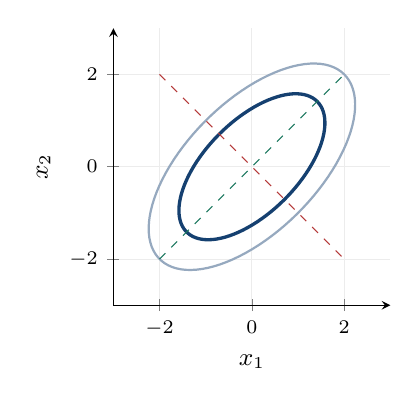
\begin{tikzpicture}
\begin{axis}[base,width=8.2cm,height=5.1cm,xmin=-3,xmax=3,ymin=-3,ymax=3,xlabel={$x_1$},ylabel={$x_2$},axis equal image]
\addplot[azul,very thick,domain=0:360,variable=\t,samples=100]({sqrt(2)*cos(t)-sin(t)/sqrt(2)},{sqrt(2)*cos(t)+sin(t)/sqrt(2)});
\addplot[azul!45,thick,domain=0:360,variable=\t,samples=100]({2*cos(t)-sin(t)},{2*cos(t)+sin(t)});
\addplot[verde,dashed,domain=-2:2]{x};
\addplot[rojo,dashed,domain=-2:2]{-x};
\end{axis}
\end{tikzpicture}
\caption{$\Sigma=\begin{psmallmatrix}3&1\\1&3\end{psmallmatrix}$: autovalores $4,2$ y elipses $d_\Sigma^2=1,2$.}
\end{figure}
\begin{ejemplo}[Comprobar ejes y distancia]
Para esa matriz, $q_1=(1,1)\T/\sqrt2$, $q_2=(1,-1)\T/\sqrt2$.
Si $x=(2,0)\T$ y $\mu=0$, ambas coordenadas principales valen $\sqrt2$:
\[
d_\Sigma^2=\frac24+\frac22=\frac32,\qquad
\Sigma^{-1}=\frac18\begin{pmatrix}3&-1\\-1&3\end{pmatrix}.
\]
El producto directo $x\T\Sigma^{-1}x=12/8$ coincide.
\end{ejemplo}
Si $\Sigma$ es singular, su pseudoinversa invierte solo autovalores
positivos. Una distancia con esa pseudoinversa ignora el núcleo: debe
comprobarse aparte que el dato pertenezca al soporte afín de la distribución.

\topic{Media muestral, dependencia y ley de grandes números}{s23}
Sean $x_1,\ldots,x_n\in\R^p$ observaciones iid, de media $\mu$ y
covarianza $\Sigma$. La media muestral es
$\bar x=n^{-1}\sum_{i=1}^nx_i$.
La linealidad no necesita independencia:
\[
\E[\bar x]=\frac1n\sum_i\E[x_i]=\mu.
\]
La independencia sí interviene en su covarianza:
\[
\Cov(\bar x)
=\frac1{n^2}\sum_i\sum_j\Cov(x_i,x_j)
=\frac1{n^2}\sum_i\Sigma
=\boxed{\frac{\Sigma}{n}}.
\]
En particular,
$\Var(\bar x_r)=\Sigma_{rr}/n$ y
$\Cov(\bar x_r,\bar x_s)=\Sigma_{rs}/n$.
Un mayor tamaño de muestra reduce toda la matriz, incluidas sus entradas
fuera de la diagonal.

\textbf{Cuando las observaciones dependen.}
La fórmula doble sigue siendo exacta, pero ya no desaparecen los términos
$i\ne j$. En un caso escalar de varianza $\sigma^2$ y correlación común
$\rho$ entre pares,
\[
\Var(\bar U)=\frac{\sigma^2}{n}\{1+(n-1)\rho\}.
\]
Para que la matriz equicorrelacionada sea válida,
$-1/(n-1)\le\rho\le1$.
Si $\rho>0$ permanece fija al crecer $n$, la varianza no tiende a cero:
las observaciones comparten una fuente de incertidumbre.

\begin{deduccion}
La identidad $\E[\norm{\bar x-\mu}_2^2]=\tr(\Sigma)/n$,
junto con la desigualdad de Markov para la variable no negativa
$\norm{\bar x-\mu}_2^2$, produce
\[
\Prob(\norm{\bar x-\mu}_2>\varepsilon)
\le \frac{\tr(\Sigma)}{n\varepsilon^2}\longrightarrow0.
\]
Así se demuestra una ley débil de grandes números para $p$ fijo y segundos
momentos finitos, sin presuponer el resultado.
\end{deduccion}

\textbf{Distribución exacta bajo normalidad.}
Si $x_i\sim\Normal_p(\mu,\Sigma)$ son independientes,
\[
\bar x\sim\Normal_p(\mu,\Sigma/n),\qquad
\sqrt n(\bar x-\mu)\sim\Normal_p(0,\Sigma).
\]
La afirmación es exacta para todo $n$. Sin normalidad, el teorema central
del límite dará la segunda distribución solamente en el límite.

\begin{ejemplo}[Dos medias que siguen correlacionadas]
Con $\Sigma=\begin{psmallmatrix}4&2\\2&9\end{psmallmatrix}$ y $n=100$,
\[
\Cov(\bar x)=\begin{pmatrix}.04&.02\\.02&.09\end{pmatrix},
\quad \operatorname{se}(\bar x_1)=.2,\quad
\operatorname{se}(\bar x_2)=.3.
\]
$\Corr(\bar x_1,\bar x_2)=.02/(.2\cdot.3)=1/3$,
igual que la correlación poblacional. La escala disminuye; la correlación
de las dos medias se conserva.
\end{ejemplo}
La dimensión importa: la cota usa $\tr\Sigma$, que puede aumentar con $p$.
Decir simplemente que $n$ es grande no garantiza precisión conjunta en
muchas coordenadas.

\topic{Covarianza muestral: por qué aparece n menos uno}{s24}
Con datos iid de segundo momento finito, definimos
\[
S=\frac1{n-1}\sum_{i=1}^n(x_i-\bar x)(x_i-\bar x)\T,\qquad n\ge2.
\]
Para demostrar insesgamiento no basta afirmar que se pierde un grado de
libertad: hay que calcular la esperanza.

\begin{deduccion}
Escribamos $z_i=x_i-\mu$ y $\bar z=\bar x-\mu$. Al expandir y usar
$\sum_i z_i=n\bar z$,
\[
\sum_i(z_i-\bar z)(z_i-\bar z)\T
=\sum_i z_iz_i\T-n\bar z\bar z\T.
\]
Tomando esperanza,
$\E[z_iz_i\T]=\Sigma$ y
$\E[\bar z\bar z\T]=\Sigma/n$. Así,
\[
\E\!\left[\sum_i(x_i-\bar x)(x_i-\bar x)\T\right]
=n\Sigma-n(\Sigma/n)=(n-1)\Sigma,\qquad
\boxed{\E[S]=\Sigma}.
\]
La matriz con denominador $n$ tiene esperanza $(1-1/n)\Sigma$.
Si la media poblacional fuera conocida, centrar en $\mu$ y dividir por
$n$ sí sería insesgado.
\end{deduccion}

\textbf{Centrar por una matriz.}
Si la tabla $D$ tiene las observaciones en filas, sea
$H=I_n-\ones\ones\T/n$ y $D_c=HD$. Entonces
\[
H\T=H,\quad H^2=H,\quad H\ones=0,\quad \rank(H)=n-1,
\qquad S=\frac{D\T HD}{n-1}=\frac{D_c\T D_c}{n-1}.
\]
El centrado es una proyección en el espacio de las $n$ observaciones.
No es la misma proyección que PCA en el espacio de las $p$ variables.

\begin{ejemplo}[Seis datos, dos variables, ninguna caja negra]
Tomemos filas $(2,1),(1,2),(-2,-1),(-1,-2),(1,-1),(-1,1)$.
La media de ambas columnas es cero y
\[
\sum_i x_{i1}^2=4+1+4+1+1+1=12,\qquad
\sum_i x_{i2}^2=12,
\]
\[
\sum_i x_{i1}x_{i2}=2+2+2+2-1-1=6.
\]
Por tanto,
$S=\frac15\begin{psmallmatrix}12&6\\6&12\end{psmallmatrix}$.
La correlación muestral es $6/\sqrt{12\cdot12}=1/2$.
\end{ejemplo}
\textbf{Positividad y rango.}
Para todo $a$, $a\T Sa=\norm{D_ca}_2^2/(n-1)\ge0$.
Además,
\[
\rank(S)=\rank(D_c)\le\min(p,n-1).
\]
Una covarianza muestral no puede ser invertible cuando $p\ge n$,
aunque la covarianza poblacional sí sea definida positiva.
Usar $n$ en lugar de $n-1$ cambia la escala, pero no el rango ni
los autovectores.

\topic{Wishart y covarianza entre covarianzas}{s25}
Para $z_1,\ldots,z_\nu$ iid $\Normal_p(0,\Sigma)$,
la matriz $W=\sum_{a=1}^\nu z_az_a\T$ tiene distribución Wishart
$\mathcal W_p(\Sigma,\nu)$ \cite{wishart}. Esta definición sigue siendo válida si
$\nu<p$; en ese caso la matriz es singular.
Se ve inmediatamente que $\E[W]=\nu\Sigma$.

\textbf{Covarianza de todas las entradas.}
Al expandir $W_{ij}=\sum_a z_{ai}z_{aj}$, términos con $a\ne b$
tienen covarianza cero por independencia.
La fórmula gaussiana de cuarto orden da
\[
\Cov(z_i z_j,z_r z_s)
=\Sigma_{ir}\Sigma_{js}+\Sigma_{is}\Sigma_{jr}.
\]
Por tanto,
\[
\boxed{\Cov(W_{ij},W_{rs})
=\nu(\Sigma_{ir}\Sigma_{js}+\Sigma_{is}\Sigma_{jr})}.
\]
Esta es una covarianza entre \emph{estimadores de covarianzas}, no
entre las variables originales.

\textbf{La covarianza muestral normal.}
Si $D=\ones\mu\T+G L\T$ con $G$ de entradas iid normales,
una matriz ortogonal $O$ con primera fila $\ones\T/\sqrt n$ transforma
$H$ en $\diag(0,I_{n-1})$. Las filas de $OG$ siguen siendo iid normales
estándar. La primera determina $\bar x$; las restantes determinan $S$:
\[
(n-1)S\sim\mathcal W_p(\Sigma,n-1),\qquad \bar x\ \perp\ S.
\]
Aquí $\perp$ indica independencia, que procede de bloques gaussianos
ortogonales. Escribiendo $\nu=n-1$,
\[
\boxed{\Cov(S_{ij},S_{rs})
=\frac{\Sigma_{ir}\Sigma_{js}+\Sigma_{is}\Sigma_{jr}}{\nu}},
\quad
\Var(S_{ij})=\frac{\Sigma_{ii}\Sigma_{jj}+\Sigma_{ij}^2}{\nu}.
\]

\begin{ejemplo}[Covarianzas de segundo nivel]
Con $\Sigma=\begin{psmallmatrix}4&1\\1&9\end{psmallmatrix}$ y $n=11$,
\[
\Var(S_{11})=2(4)^2/10=3.2,\quad
\Var(S_{22})=16.2,\quad \Var(S_{12})=(36+1)/10=3.7,
\]
\[
\Cov(S_{11},S_{22})=2(1)^2/10=.2,\qquad
\Cov(S_{11},S_{12})=2(4)(1)/10=.8.
\]
No es correcto tratar todas las entradas estimadas de $S$ como independientes.
\end{ejemplo}
Si $K_p$ es la matriz de conmutación que cumple
$K_p\vecop(A)=\vecop(A\T)$, la misma fórmula es
\[
\Cov(\vecop S)=\frac1\nu(I_{p^2}+K_p)(\Sigma\otimes\Sigma).
\]
La simetría hace singular esta covarianza de tamaño $p^2$: las entradas
$S_{ij}$ y $S_{ji}$ son idénticas.
Sin normalidad, la fórmula exacta requiere cuartos momentos y contiene
términos adicionales; insesgamiento de $S$ no implica distribución Wishart.


\begin{figure}[H]\centering
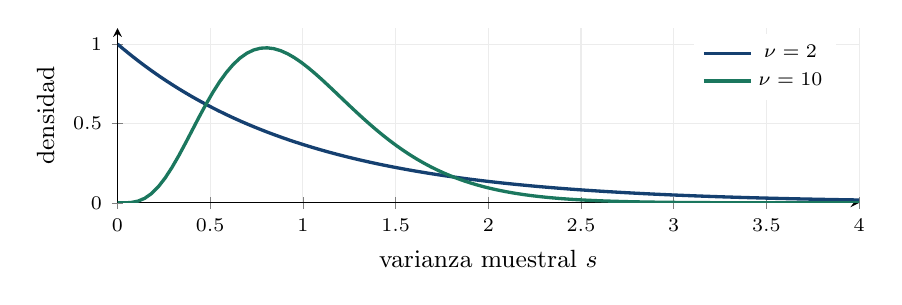
\begin{tikzpicture}
\begin{axis}[base,width=11cm,height=3.8cm,xmin=0,xmax=4,ymin=0,ymax=1.1,xlabel={varianza muestral $s$},ylabel={densidad},legend pos=north east]
\addplot[curva,domain=0:4]{exp(-x)};\addlegendentry{$\nu=2$}
\addplot[verde,very thick,domain=0:4]{3125*x^4*exp(-5*x)/24};\addlegendentry{$\nu=10$}
\end{axis}
\end{tikzpicture}
\caption{Para varianza poblacional uno, $\nu S_{11}\sim\chi^2_\nu$: ambas medias son uno, pero las varianzas son $2/\nu$.}
\end{figure}
\topic{Muchas dimensiones: singularidad y regularización}{s26}
Una matriz simétrica de orden $p$ contiene $p(p+1)/2$ entradas distintas.
Aumentar $p$ multiplica el número de momentos que hay que estimar.
Si $p\ge n$, $\rank(S)\le n-1$ impide invertir $S$:
la información muestral no identifica todas las direcciones de dispersión.

\textbf{Error conjunto.} Bajo normalidad, $S$ es insesgada y
la fórmula anterior permite sumar las varianzas:
\[
\E[\norm{S-\Sigma}\F^2]
=\sum_{i,j}\Var(S_{ij})
=\boxed{\frac{(\tr\Sigma)^2+\tr(\Sigma^2)}{n-1}}.
\]
La primera suma es $\sum_{i,j}\Sigma_{ii}\Sigma_{jj}=(\tr\Sigma)^2$;
la segunda es $\sum_{i,j}\Sigma_{ij}^2=\tr(\Sigma^2)$.
Si $\Sigma=I_p$, el error esperado es $(p^2+p)/(n-1)$.
La precisión de cada entrada no garantiza precisión de la matriz entera.

\textbf{Contracción hacia un objetivo fijo.}
Sea $T=\tau I_p$ con $\tau>0$ fijo. Para $0\le\delta\le1$,
\[
S_\delta=(1-\delta)S+\delta T,\qquad
\E[S_\delta]-\Sigma=\delta(T-\Sigma).
\]
Si $\delta>0$, para todo $a\ne0$,
$a\T S_\delta a\ge\delta\tau\norm a_2^2>0$:
la matriz es invertible incluso cuando $S$ no lo es.
Sus autovalores son $(1-\delta)\widehat\lambda_j+\delta\tau$.

\begin{deduccion}
Sea $V=\E[\norm{S-\Sigma}\F^2]$ y $B=\norm{T-\Sigma}\F^2$.
Al expandir el cuadrado, el término cruzado es cero por
$\E[S-\Sigma]=0$:
\[
R(\delta)=\E[\norm{S_\delta-\Sigma}\F^2]
=(1-\delta)^2V+\delta^2B.
\]
Derivar $R$ da $-2(1-\delta)V+2\delta B=0$:
\[
\boxed{\delta_*=\frac{V}{V+B}}.
\]
Es una intensidad \emph{oráculo}: depende de $\Sigma$, desconocida.
Un objetivo o una intensidad estimados introducen términos adicionales;
esta fórmula no se aplica ignorando su aleatoriedad.
\end{deduccion}
\begin{ejemplo}[Rango insuficiente y raíz estable]
Si $S=\diag(3,1,0)$, $T=I_3$ y $\delta=.2$,
$S_\delta=\diag(2.6,1,.2)$ es invertible.
Su inversa es $\diag(1/2.6,1,5)$.
El menor autovalor tiene un piso positivo; la contracción altera
deliberadamente la estimación para controlar inestabilidad.
\end{ejemplo}
Para blanqueamiento se puede usar
$(S+\lambda I)^{-1/2}$: cada dirección recibe factor
$(\widehat\lambda_j+\lambda)^{-1/2}$.
Pseudoinvertir usa cero en las direcciones nulas; regularizar usa un piso.
Son decisiones matemáticas distintas, con efectos distintos sobre
distancias, coeficientes y covarianzas de estimadores.

\begin{figure}[H]\centering
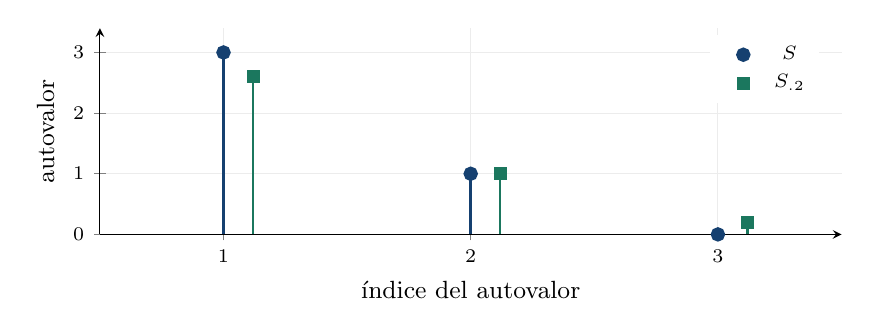
\begin{tikzpicture}
\begin{axis}[base,width=11cm,height=4.2cm,xmin=.5,xmax=3.5,ymin=0,ymax=3.4,xtick={1,2,3},xlabel={índice del autovalor},ylabel={autovalor},legend pos=north east]
\addplot[ycomb,mark=*,azul,very thick]coordinates{(1,3)(2,1)(3,0)};\addlegendentry{$S$}
\addplot[ycomb,mark=square*,verde,thick]coordinates{(1.12,2.6)(2.12,1)(3.12,.2)};\addlegendentry{$S_{.2}$}
\end{axis}
\end{tikzpicture}
\caption{El objetivo identidad crea un piso positivo para el modo que no tenía varianza muestral.}
\end{figure}
\topic{Teorema espectral y cociente de Rayleigh}{s27}
Sea $A=A\T\in\R^{p\times p}$. Un autovector $q\ne0$ satisface
$Aq=\lambda q$. El escalar $\lambda$ es el autovalor:
la transformación cambia la escala de esa dirección sin girarla.
El teorema espectral afirma que existe una base ortonormal de autovectores.

\begin{deduccion}
La función continua $f(q)=q\T Aq$ alcanza un máximo en la esfera compacta
$\{q:q\T q=1\}$. Para cualquier $h$ perpendicular al maximizador $q_1$,
la curva $(q_1+th)/\norm{q_1+th}$ permanece en la esfera.
Su derivada de $f$ en $t=0$ es $2h\T Aq_1=0$.
Luego $Aq_1$ es perpendicular a todo el complemento de $q_1$:
$Aq_1=\lambda_1q_1$, con $\lambda_1=q_1\T Aq_1$.
Además, el complemento es invariante:
\[
q_1\T Ah=(Aq_1)\T h=\lambda_1q_1\T h=0.
\]
La restricción de $A$ a ese subespacio sigue siendo simétrica.
Repitiendo el argumento en dimensión $p-1$ y por inducción hasta dimensión
uno, obtenemos $p$ autovectores ortonormales.
\end{deduccion}
Al reunirlos en $Q=[q_1,\ldots,q_p]$ y ordenar
$\lambda_1\ge\cdots\ge\lambda_p$,
\[
AQ=Q\Lambda,\quad Q\T Q=QQ\T=I_p,\qquad
\boxed{A=Q\Lambda Q\T}.
\]
La demostración establece autovalores reales y una diagonalización
ortogonal. Una matriz no simétrica no cumple necesariamente estas propiedades.

\textbf{Rayleigh.} Para $a\ne0$, el cociente
$R_A(a)=a\T Aa/(a\T a)$ no cambia al multiplicar $a$ por un escalar
no nulo. Escribiendo $a=Qc$,
\[
R_A(a)=\frac{\sum_j\lambda_jc_j^2}{\sum_jc_j^2},
\quad
\lambda_p\le R_A(a)\le\lambda_1.
\]
Es un promedio ponderado de autovalores. Sus extremos se alcanzan en
los autovectores respectivos. Si $A=\Sigma\succeq0$,
todos los autovalores son no negativos, porque
$\lambda_j=q_j\T\Sigma q_j\ge0$.
\[
\tr(A)=\sum_j\lambda_j,\quad \det A=\prod_j\lambda_j,\quad
A^{-1}=Q\diag(\lambda_j^{-1})Q\T
\]
cuando no hay autovalores nulos.

\begin{ejemplo}[Calcular el sistema propio desde el determinante]
Para $A=\begin{psmallmatrix}3&1\\1&3\end{psmallmatrix}$,
\[
\det(A-\lambda I)=(3-\lambda)^2-1
=(\lambda-4)(\lambda-2).
\]
Para $\lambda=4$, $-q_1+q_2=0$; para $\lambda=2$, $q_1+q_2=0$.
Normalizar produce $(1,1)\T/\sqrt2$ y $(1,-1)\T/\sqrt2$.
\end{ejemplo}
Autovectores de autovalores distintos son ortogonales:
$q_i\T Aq_j=\lambda_jq_i\T q_j=\lambda_iq_i\T q_j$.
Con autovalores repetidos, la base dentro del espacio propio no es única.
Los valores de varianza pueden ser identificables aunque un eje particular
no lo sea.


\begin{figure}[H]\centering
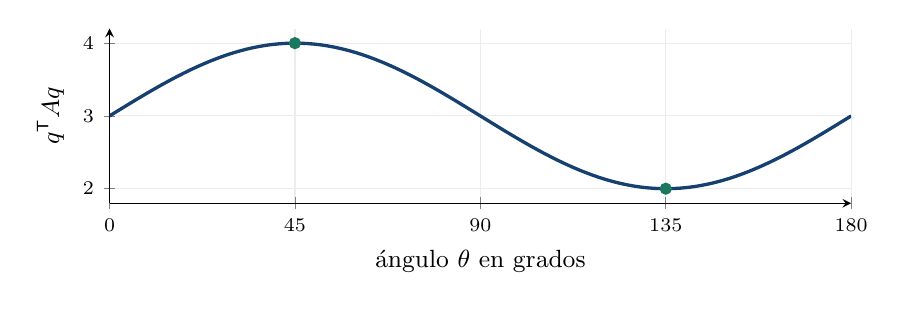
\begin{tikzpicture}
\begin{axis}[base,width=11cm,height=3.8cm,xmin=0,xmax=180,ymin=1.8,ymax=4.2,xtick={0,45,90,135,180},xlabel={ángulo $\theta$ en grados},ylabel={$q^\mathsf T A q$}]
\addplot[curva,domain=0:180]{3+sin(2*x)};
\addplot[only marks,mark=*,verde]coordinates{(45,4)(135,2)};
\end{axis}
\end{tikzpicture}
\caption{Para $q=(\cos\theta,\sin\theta)^\mathsf T$ y $A=\left(\begin{smallmatrix}3&1\\1&3\end{smallmatrix}\right)$, Rayleigh alcanza $4$ y $2$.}
\end{figure}
\topic{PCA: máxima varianza y mínima reconstrucción}{s28}
Sea $x$ de media $\mu$ y covarianza $\Sigma$.
La coordenada en una dirección unitaria $q$ es
$z=q\T(x-\mu)$, de media cero y varianza $q\T\Sigma q$.
La primera componente principal resuelve
\[
\max_{q\T q=1}q\T\Sigma q.
\]
El lagrangiano $\mathcal L=q\T\Sigma q-\lambda(q\T q-1)$ tiene
gradiente $2\Sigma q-2\lambda q$. Por tanto,
$\Sigma q=\lambda q$, y Rayleigh selecciona el mayor autovalor.

\textbf{Varias componentes simultáneas.}
Para $Q_k=[q_1,\ldots,q_k]$ con $Q_k\T Q_k=I_k$,
\[
z=Q_k\T(x-\mu),\quad
\E[z]=0,\quad \Cov(z)=Q_k\T\Sigma Q_k=\Lambda_k.
\]
Las coordenadas son incorrelacionadas; serán independientes si $x$ es
normal. La varianza conjunta retenida es $\tr(Q_k\T\Sigma Q_k)$.

\begin{deduccion}
Para cualquier matriz $W$ de $k$ columnas ortonormales, sea
$a_j=\norm{W\T q_j}_2^2$. Cada $a_j$ está en $[0,1]$ y
$\sum_ja_j=\tr(WW\T)=k$.
Por ello,
\[
\tr(W\T\Sigma W)=\sum_j\lambda_ja_j\le\sum_{j=1}^k\lambda_j.
\]
El máximo se consigue asignando peso uno a los primeros $k$ ejes.
Esta es la demostración de optimalidad conjunta, no solamente de
la primera componente.
\end{deduccion}
\textbf{Reconstrucción.}
$\widehat x=\mu+Q_kz=\mu+P_k(x-\mu)$, $P_k=Q_kQ_k\T$.
Como $(I-P_k)$ es una proyección,
\[
\E[\norm{x-\widehat x}_2^2]
=\tr((I-P_k)\Sigma)
=\boxed{\sum_{j>k}\lambda_j}.
\]
Maximizar varianza retenida equivale a minimizar error cuadrático
de reconstrucción. Las varianzas de la reconstrucción y del error son
\[
\Cov(\widehat x)=Q_k\Lambda_kQ_k\T,\quad
\Cov(x-\widehat x)=Q_{>k}\Lambda_{>k}Q_{>k}\T,
\quad \Cov(\widehat x,x-\widehat x)=0.
\]
\begin{ejemplo}[Dos ejes y una reducción]
Con $\Sigma=\begin{psmallmatrix}3&1\\1&3\end{psmallmatrix}$,
retener $q_1=(1,1)\T/\sqrt2$ conserva $4/(4+2)=2/3$ de la varianza.
Para $x-\mu=(3,1)\T$, $z=2\sqrt2$ y la reconstrucción centrada es
$(2,2)\T$. El error es $(1,-1)\T$.
\end{ejemplo}
\textbf{Escalas.} Si se estandariza $x$ con
$D_\sigma=\diag(\sqrt{\Sigma_{11}},\ldots,\sqrt{\Sigma_{pp}})$,
la matriz usada es $R=D_\sigma^{-1}\Sigma D_\sigma^{-1}$.
PCA sobre $R$ optimiza en unidades estandarizadas; PCA sobre $\Sigma$
optimiza en las unidades originales. No dan necesariamente los mismos ejes.
PCA modela dispersión de predictores, no su utilidad para explicar $y$.

\topic{SVD, pseudoinversa y aproximación de rango bajo}{s29}
Sea $D_c\in\R^{n\times p}$ de rango $r$.
La matriz $D_c\T D_c$ es simétrica positiva y tiene $r$ autovalores
positivos $s_j^2$ con autovectores ortonormales $v_j$.
Definamos $u_j=D_cv_j/s_j$. Entonces
\[
u_i\T u_j=\frac{v_i\T D_c\T D_cv_j}{s_is_j}=\delta_{ij}.
\]
Si $v$ está en el núcleo de $D_c\T D_c$, $\norm{D_cv}^2=0$;
por ello, esos autovectores no contribuyen a $D_c$.
Resulta la SVD reducida:
\[
\boxed{D_c=U_r\mathcal S_rV_r\T
=\sum_{j=1}^rs_ju_jv_j\T},
\quad \mathcal S_r=\diag(s_1,\ldots,s_r),\ s_1\ge\cdots\ge s_r>0.
\]
$U_r$ es $n\times r$, $V_r$ es $p\times r$ y
$\mathcal S_r$ es $r\times r$. Los vectores singulares izquierdos viven
en observaciones; los derechos viven en variables.

\textbf{Puente con PCA.}
\[
S=\frac{D_c\T D_c}{n-1}
=V_r\diag\!\left(\frac{s_j^2}{n-1}\right)V_r\T,\quad
\lambda_j=\frac{s_j^2}{n-1},\qquad D_cV_r=U_r\mathcal S_r.
\]
Las puntuaciones no son $V_r$: son $D_cV_r$.
La pseudoinversa
$D_c^+=V_r\mathcal S_r^{-1}U_r\T$
invierte los valores singulares positivos y deja en cero el núcleo.
$D_cD_c^+=U_rU_r\T$ y $D_c^+D_c=V_rV_r\T$ son proyecciones.

\begin{teorema}[Mejor aproximación en norma de Frobenius]
Para $k\le r$, $D_k=\sum_{j=1}^ks_ju_jv_j\T$ minimiza
$\norm{D_c-B}\F^2$ entre matrices $B$ de rango a lo sumo $k$.
El error mínimo es $\sum_{j>k}s_j^2$.
\end{teorema}
\begin{deduccion}
Sea $P$ la proyección sobre el espacio de filas de $B$; tiene rango
a lo sumo $k$ y $B=BP$.
\[
D_c-B=D_c(I-P)+(D_cP-B).
\]
Los dos sumandos son ortogonales en Frobenius porque
$(I-P)P=0$. Luego
\[
\norm{D_c-B}\F^2\ge\norm{D_c(I-P)}\F^2
=\tr(D_c\T D_c)-\tr(PD_c\T D_c)
\ge\sum_{j>k}s_j^2.
\]
La última desigualdad es la optimalidad de las primeras direcciones
espectrales. Para $B=D_k$, la cota se alcanza.
\end{deduccion}
\begin{ejemplo}[Pseudoinversa y truncación son diferentes]
$D=\diag(3,1,0)$ tiene $D^+=\diag(1/3,1,0)$.
Su aproximación de rango uno es $D_1=\diag(3,0,0)$ y el error
Frobenius al cuadrado es $1$.
La pseudoinversa conserva la segunda dirección; la truncación la descarta.
\end{ejemplo}
Formar $D_c\T D_c$ eleva al cuadrado el número de condición:
$s_1^2/s_r^2=(s_1/s_r)^2$.
Por eso, calcular directamente la SVD puede ser más estable que
diagonalizar productos cruzados.

\topic{Laboratorio exacto de PCA y SVD}{s30}
Usamos los seis datos de la sección \ref{s24}. La media es cero:
\[
D=\begin{pmatrix}2&1\\1&2\\-2&-1\\-1&-2\\1&-1\\-1&1\end{pmatrix},
\quad D\T D=\begin{pmatrix}12&6\\6&12\end{pmatrix},
\quad S=\frac15D\T D.
\]
El polinomio característico es
$(12/5-\lambda)^2-(6/5)^2$.
Por tanto,
\[
\lambda_1=18/5,\quad \lambda_2=6/5,\qquad
Q=\frac1{\sqrt2}\begin{pmatrix}1&1\\1&-1\end{pmatrix}.
\]
Las puntuaciones $T=DQ$ se calculan sumando y restando cada fila:
\[
T=\frac1{\sqrt2}
\begin{pmatrix}3&1\\3&-1\\-3&-1\\-3&1\\0&2\\0&-2\end{pmatrix},
\quad T\T T=\begin{pmatrix}18&0\\0&6\end{pmatrix}.
\]
La primera columna tiene varianza muestral $18/5$ y la segunda $6/5$;
su covarianza es cero. Retener la primera conserva $18/(18+6)=75\%$.

\textbf{La SVD completa del ejemplo.}
$s_1=\sqrt{18}=3\sqrt2$, $s_2=\sqrt6$ y
\[
U=\begin{pmatrix}
1/2&1/\sqrt{12}\\1/2&-1/\sqrt{12}\\
-1/2&-1/\sqrt{12}\\-1/2&1/\sqrt{12}\\
0&1/\sqrt3\\0&-1/\sqrt3
\end{pmatrix},\quad
D=U\diag(3\sqrt2,\sqrt6)Q\T.
\]
Comprobar $U\T U=I_2$ y $Q\T Q=I_2$ verifica las normalizaciones.
La reconstrucción de rango uno es
\[
D_1=T_{\cdot1}q_1\T
=\begin{pmatrix}1.5&1.5\\1.5&1.5\\-1.5&-1.5\\-1.5&-1.5\\0&0\\0&0\end{pmatrix}.
\]
El error total es $\norm{D-D_1}\F^2=6$, y $6/(n-1)=6/5$
coincide con el autovalor descartado.

\begin{figure}[H]\centering
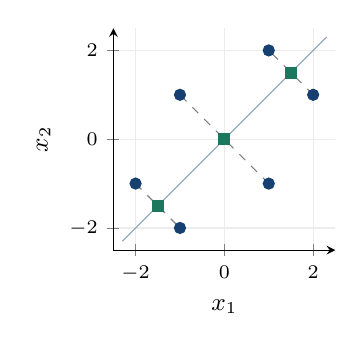
\begin{tikzpicture}
\begin{axis}[base,width=10cm,height=4.4cm,xmin=-2.5,xmax=2.5,ymin=-2.5,ymax=2.5,xlabel={$x_1$},ylabel={$x_2$},axis equal image]
\addplot[azul!50,domain=-2.3:2.3]{x};
\addplot[only marks,mark=*,azul]coordinates{(2,1)(1,2)(-2,-1)(-1,-2)(1,-1)(-1,1)};
\addplot[only marks,mark=square*,verde]coordinates{(1.5,1.5)(-1.5,-1.5)(0,0)};
\addplot[gray,dashed]coordinates{(2,1)(1.5,1.5)(1,2)};
\addplot[gray,dashed]coordinates{(-2,-1)(-1.5,-1.5)(-1,-2)};
\addplot[gray,dashed]coordinates{(1,-1)(0,0)(-1,1)};
\end{axis}
\end{tikzpicture}
\caption{Datos (círculos) y reconstrucciones (cuadrados): proyección perpendicular sobre el primer eje.}
\end{figure}
Un nuevo dato $x=(3,0)\T$ tiene coordenadas
$(3/\sqrt2,3/\sqrt2)\T$. Su reconstrucción de rango uno es
$(1.5,1.5)\T$; no hay que volver a estimar PCA para transformarlo.

\topic{Incertidumbre de autovalores y autovectores}{s31}
Los ejes poblacionales son fijos; los de $S$ son estimadores.
Supongamos $\Sigma q_j=\lambda_jq_j$, $\norm{q_j}=1$ y
$\lambda_j$ distinto de los demás.
Escribamos $S=\Sigma+E$ y perturbemos
$\widehat\lambda_j=\lambda_j+\delta\lambda_j$,
$\widehat q_j=q_j+\delta q_j$.
La normalización implica $q_j\T\delta q_j=0$ a primer orden.

\begin{deduccion}
Al expandir $(\Sigma+E)(q_j+\delta q_j)
=(\lambda_j+\delta\lambda_j)(q_j+\delta q_j)$ y omitir productos
de segundo orden,
\[
(\Sigma-\lambda_jI)\delta q_j
=-Eq_j+\delta\lambda_jq_j.
\]
Multiplicar por $q_j\T$ da
$\delta\lambda_j=q_j\T Eq_j$.
Multiplicar por $q_\ell\T$, $\ell\ne j$, da
\[
\boxed{\delta q_j
=\sum_{\ell\ne j}
\frac{q_\ell\T Eq_j}{\lambda_j-\lambda_\ell}\,q_\ell}.
\]
La cercanía entre autovalores amplifica las perturbaciones de los ejes.
\end{deduccion}
\textbf{Covarianzas gaussianas aproximadas.}
En la base propia, la matriz poblacional es diagonal.
La fórmula Wishart con $\nu=n-1$ produce
\[
\Var(q_j\T Eq_j)=\frac{2\lambda_j^2}{\nu},\qquad
\Var(q_\ell\T Eq_j)=\frac{\lambda_\ell\lambda_j}{\nu}
\quad(\ell\ne j).
\]
Por el CLT de los productos y el método delta, para $p$ fijo y brechas
espectrales positivas,
\[
\sqrt n(\widehat\lambda_j-\lambda_j)
\dto\Normal(0,2\lambda_j^2),
\]
\[
\Cov(\widehat q_j-q_j)\approx
\frac1n\sum_{\ell\ne j}
\frac{\lambda_j\lambda_\ell}{(\lambda_j-\lambda_\ell)^2}
q_\ell q_\ell\T.
\]
Se alinea el signo de $\widehat q_j$ con $q_j$ antes de comparar.
Estas son aproximaciones, no momentos exactos de autovectores muestrales.

\begin{ejemplo}[Una brecha pequeña cambia la precisión]
Con autovalores $4,2$ y $n=100$, la varianza angular de primer orden
del primer eje es $4\cdot2/[100(4-2)^2]=.02$.
Con autovalores $4,3.9$, pasa a
$4\cdot3.9/[100(.1)^2]=15.6$.
La aproximación local deja de ser útil cuando su dispersión es tan grande.
\end{ejemplo}
\begin{cuidado}[Repetición y sesgo]
Si $\lambda_j=\lambda_\ell$, no hay un eje único dentro del espacio propio
y la fórmula con denominador cero no se aplica. Puede estudiarse el
subespacio completo. Además, $\E[S]=\Sigma$ no implica
$\E[\widehat q_j]=q_j$ ni $\E[\widehat\lambda_j]=\lambda_j$:
diagonalizar es una operación no lineal.
\end{cuidado}

\begin{figure}[H]\centering
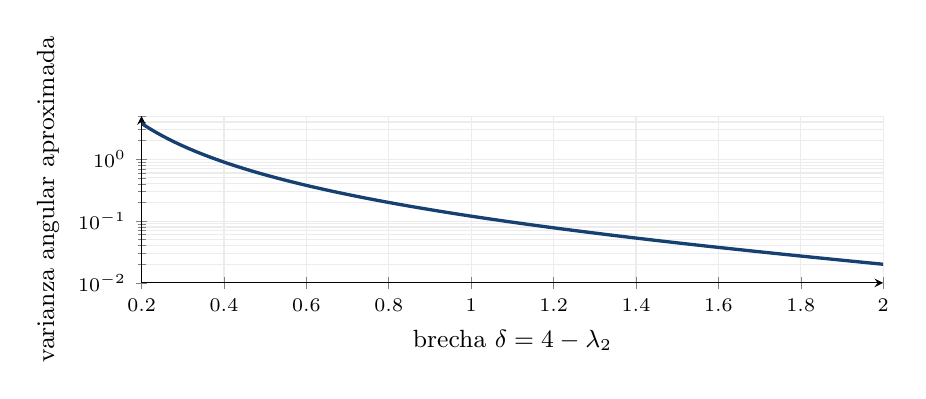
\begin{tikzpicture}
\begin{semilogyaxis}[base,width=11cm,height=3.7cm,xmin=.2,xmax=2,ymin=.01,ymax=5,xlabel={brecha $\delta=4-\lambda_2$},ylabel={varianza angular aproximada}]
\addplot[curva,domain=.2:2]{4*(4-x)/(100*x*x)};
\end{semilogyaxis}
\end{tikzpicture}
\caption{Con $\lambda_1=4,n=100$, una brecha pequeña amplifica la incertidumbre del eje; la aproximación es local.}
\end{figure}
\topic{PCR y ridge: esperanza, sesgo y covarianza}{s32}
Fijemos un diseño $X\in\R^{n\times k}$ de rango $k$, con
$y=X\beta+u$, $\E[u\mid X]=0$ y $\Cov(u\mid X)=\sigma^2I_n$.
Para simplificar la penalización, no incluimos un intercepto en este bloque.
Sea $X=U\mathcal S V\T$ su SVD, con $s_j>0$.

\textbf{Regresión por componentes principales (PCR).}
Retener los primeros $m$ ejes define
\[
\widehat\beta_{\mathrm{PCR}}
=V_m\mathcal S_m^{-1}U_m\T y.
\]
Multiplicar por $X\beta$ y aplicar la regla afín da
\[
\E[\widehat\beta_{\mathrm{PCR}}\mid X]=V_mV_m\T\beta=P_m\beta,
\quad
\operatorname{sesgo}_{\mathrm{PCR}}=-(I-P_m)\beta,
\]
\[
\boxed{\Cov(\widehat\beta_{\mathrm{PCR}}\mid X)
=\sigma^2V_m\diag(s_1^{-2},\ldots,s_m^{-2})V_m\T}.
\]
Las coordenadas descartadas tienen varianza estimadora cero, pero
pueden tener sesgo no nulo.

\textbf{Ridge.} Minimizar $\norm{y-Xb}^2+\lambda\norm b^2$, $\lambda>0$,
da $-2X\T y+2(X\T X+\lambda I)b=0$. Por tanto,
\[
\widehat\beta_\lambda=(X\T X+\lambda I)^{-1}X\T y
=V\diag\!\left(\frac{s_j}{s_j^2+\lambda}\right)U\T y.
\]
Si $F_\lambda=V\diag(s_j^2/(s_j^2+\lambda))V\T$,
\[
\E[\widehat\beta_\lambda\mid X]=F_\lambda\beta,\qquad
\operatorname{sesgo}_\lambda=-\lambda(X\T X+\lambda I)^{-1}\beta,
\]
\[
\boxed{\Cov(\widehat\beta_\lambda\mid X)
=\sigma^2V\diag\!\left(\frac{s_j^2}{(s_j^2+\lambda)^2}\right)V\T}.
\]
Para la coordenada propia $\theta_j=v_j\T\beta$, la contribución a su MSE es
\[
\left(\frac{\lambda}{s_j^2+\lambda}\right)^2\theta_j^2+
\sigma^2\frac{s_j^2}{(s_j^2+\lambda)^2}.
\]
No hay una intensidad óptima universal independiente de señal y ruido.

\begin{figure}[H]\centering
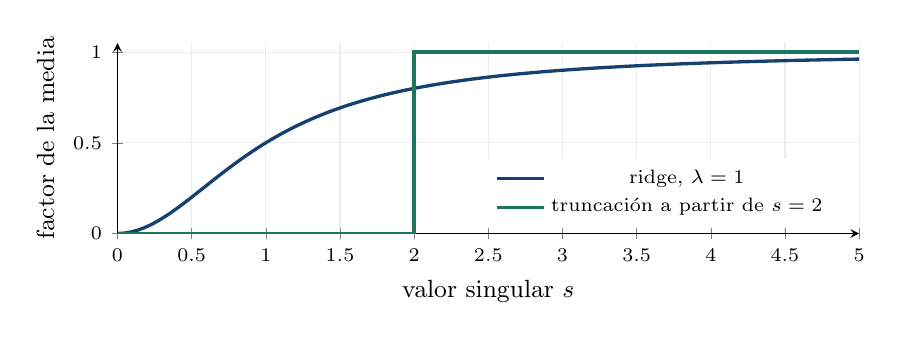
\begin{tikzpicture}
\begin{axis}[base,width=11cm,height=4cm,xmin=0,xmax=5,ymin=0,ymax=1.05,xlabel={valor singular $s$},ylabel={factor de la media},legend pos=south east]
\addplot[curva,domain=0:5]{x*x/(x*x+1)};\addlegendentry{ridge, $\lambda=1$}
\addplot[verde,very thick]coordinates{(0,0)(2,0)(2,1)(5,1)};\addlegendentry{truncación a partir de $s=2$}
\end{axis}
\end{tikzpicture}
\caption{Ridge atenúa continuamente; PCR conserva o descarta direcciones.}
\end{figure}
Si dos estimadores usan el mismo $y$ y son $A_1y,A_2y$,
$\Cov(A_1y,A_2y\mid X)=\sigma^2A_1A_2\T$.
No son independientes por calcularse con métodos distintos.
Con intercepto, se centra o se usa una penalización con cero en su posición;
penalizarlo cambia el problema.

\topic{MCO desde la función objetivo}{s33}
En el modelo lineal,
\[
\underbrace y_{n\times1}
=\underbrace X_{n\times k}\underbrace\beta_{k\times1}
+\underbrace u_{n\times1}.
\]
Cada fila es $y_i=x_i\T\beta+u_i$.
Si hay intercepto, $x_{i1}=1$ y $\beta_1$ es su coeficiente.
Mínimos cuadrados ordinarios (MCO) elige
$\widehat\beta=\argmin_b Q(b)$ con
\[
Q(b)=(y-Xb)\T(y-Xb)
=y\T y-y\T Xb-b\T X\T y+b\T X\T Xb.
\]
Los dos términos centrales son el mismo escalar:
$y\T Xb=(y\T Xb)\T=b\T X\T y$.

\begin{deduccion}
Derivar coordenada por coordenada da
\[
\frac{\partial Q}{\partial b_j}
=-2\sum_{i=1}^nx_{ij}\left(y_i-\sum_{a=1}^kx_{ia}b_a\right).
\]
Reunir esas $k$ ecuaciones forma
$X\T(y-X\widehat\beta)=0$, llamadas ecuaciones normales.
Si $\rank(X)=k$, $K=X\T X\succ0$ y
\[
\boxed{\widehat\beta=(X\T X)^{-1}X\T y}.
\]
La Hessiana es $2K\succ0$.
Además, para cualquier $h$,
$Q(\widehat\beta+h)=Q(\widehat\beta)+h\T Kh$,
porque el término cruzado contiene $X\T(y-X\widehat\beta)=0$.
Esto prueba el mínimo global único.
\end{deduccion}
Definamos
\[
A=(X\T X)^{-1}X\T\in\R^{k\times n},\quad AX=I_k,
\quad P_X=XA=X(X\T X)^{-1}X\T\in\R^{n\times n}.
\]
Los valores ajustados son $\widehat y=P_Xy$ y los residuos
$\widehat u=(I_n-P_X)y=M_Xy$.
$P_X$ y $M_X$ son simétricas e idempotentes, y
$P_XM_X=0$. Las ecuaciones normales expresan $X\T\widehat u=0$.

\textbf{Separar álgebra de hipótesis estadísticas.}
La fórmula se calcula sin normalidad ni exogeneidad.
Para interpretarla como un estimador insesgado de $\beta$, habrá que
imponer $\E[u\mid X]=0$.
Un buen ajuste geométrico no demuestra esta condición.

\begin{ejemplo}[Por qué todas las dummies más el intercepto fallan]
Si $d_{i1}+d_{i2}=1$, las columnas de $X=[\ones,d_1,d_2]$
cumplen $X(1,-1,-1)\T=0$.
Entonces $X\T X$ no es invertible. Omitir una dummy establece la
categoría de referencia y recupera identificación si no hay otras dependencias.
\end{ejemplo}
Si hay rango insuficiente, $X^+y$ es una solución de norma mínima.
Todas las soluciones son $X^+y+h$ con $h\in\ker X$.
Los valores ajustados pueden ser únicos aunque los coeficientes no lo sean.
No existe una covarianza identificada de cada coeficiente sin fijar
restricciones o una convención adicional.

\topic{Momentos de todos los coeficientes MCO}{s34}
Condicionemos en un diseño de rango completo $X$.
Usando $y=X\beta+u$ y $AX=I_k$,
\[
\boxed{\widehat\beta=\beta+Au},\qquad
A=(X\T X)^{-1}X\T.
\]
Si $\E[u\mid X]=0$, la linealidad da
$\E[\widehat\beta\mid X]=\beta$.
Si $m(X)=\E[u\mid X]\ne0$, el sesgo condicional es $Am(X)$.

\textbf{Covarianza general.}
Sea $\Omega=\Cov(u\mid X)$. No exigimos normalidad ni homocedasticidad:
\[
\Cov(\widehat\beta\mid X)
=\E[A(u-m)(u-m)\T A\T\mid X]
=\boxed{A\Omega A\T}.
\]
Expandiendo $A$,
\[
\boxed{V_\beta=(X\T X)^{-1}X\T\Omega X(X\T X)^{-1}}.
\]
Cada entrada contiene la varianza o covarianza pedida:
\[
\Var(\widehat\beta_j\mid X)=\sum_{i,a}A_{ji}\Omega_{ia}A_{ja},
\quad
\Cov(\widehat\beta_j,\widehat\beta_r\mid X)
=\sum_{i,a}A_{ji}\Omega_{ia}A_{ra}.
\]
Si los errores son incorrelacionados pero heterocedásticos,
$\Omega=\diag(\sigma_i^2)$ y la última suma es
$\sum_i A_{ji}A_{ri}\sigma_i^2$.

\textbf{Caso homocedástico.} Si $\Omega=\sigma^2I_n$,
\[
V_\beta=\sigma^2(X\T X)^{-1}X\T X(X\T X)^{-1}
=\boxed{\sigma^2(X\T X)^{-1}}.
\]
Si $C=(X\T X)^{-1}$, entonces
$\Var(\widehat\beta_j\mid X)=\sigma^2 C_{jj}$ y
$\Cov(\widehat\beta_j,\widehat\beta_r\mid X)=\sigma^2 C_{jr}$.
La inversa completa es necesaria, no solo su diagonal.

\begin{ejemplo}[Diseño correlacionado y coeficientes con covarianza negativa]
Si
$X\T X=\begin{psmallmatrix}10&6\\6&10\end{psmallmatrix}$ y $\sigma^2=4$,
\[
(X\T X)^{-1}=\frac1{64}\begin{pmatrix}10&-6\\-6&10\end{pmatrix},
\quad
V_\beta=\begin{pmatrix}.625&-.375\\-.375&.625\end{pmatrix}.
\]
La correlación estimadora es $-.375/.625=-.6$.
Los coeficientes pueden compensarse al explicar columnas relacionadas.
\end{ejemplo}
\textbf{Distribución completa.}
Si además $u\mid X\sim\Normal_n(0,\Omega)$,
\[
\widehat\beta\mid X\sim\Normal_k(\beta,V_\beta).
\]
La normalidad es suficiente para esta distribución exacta, pero no para
las fórmulas anteriores, que solo usan dos momentos.
Para cualquier contraste $c\T\widehat\beta$,
su media es $c\T\beta$ y su varianza $c\T V_\beta c$.
Bajo normalidad, el contraste también es normal.


\begin{figure}[H]\centering
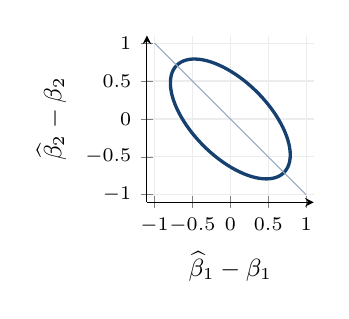
\begin{tikzpicture}
\begin{axis}[base,width=9cm,height=3.7cm,axis equal image,xmin=-1.1,xmax=1.1,ymin=-1.1,ymax=1.1,xlabel={$\widehat\beta_1-\beta_1$},ylabel={$\widehat\beta_2-\beta_2$}]
\addplot[curva,domain=0:360,variable=\t,samples=90]({sqrt(.625)*cos(t)},{-.375*cos(t)/sqrt(.625)+sqrt(.4)*sin(t)});
\addplot[azul!45,domain=-1:1]{-x};
\end{axis}
\end{tikzpicture}
\caption{Nivel de Mahalanobis uno para el ejemplo gaussiano: la covarianza negativa inclina la elipse de coeficientes.}
\end{figure}
\topic{Gauss--Markov y diseño aleatorio}{s35}
Bajo $\E[u\mid X]=0$ y $\Cov(u\mid X)=\sigma^2I_n$, MCO es
eficiente dentro de los estimadores lineales condicionalmente insesgados.
Un competidor $\widetilde\beta=By$ con $B$ fijo dado $X$ es insesgado
para todo $\beta$ si y solo si $BX=I_k$.

\begin{deduccion}
Escribamos $B=A+D$, donde $A=(X\T X)^{-1}X\T$.
Como $BX=AX=I_k$, $DX=0$.
Por tanto,
\[
AD\T=(X\T X)^{-1}X\T D\T
=(X\T X)^{-1}(DX)\T=0.
\]
Expandir la covarianza del competidor da
\[
\Cov(\widetilde\beta\mid X)
=\sigma^2(A+D)(A+D)\T
=\Cov(\widehat\beta\mid X)+\sigma^2DD\T.
\]
Para todo $c$, $c\T DD\T c=\norm{D\T c}_2^2\ge0$.
Luego la varianza de cualquier contraste del competidor es al menos
la de MCO.
\end{deduccion}
Esta es una comparación matricial en orden semidefinido.
No usa normalidad y no compara MCO con todos los estimadores sesgados.
Ridge puede reducir MSE al aceptar sesgo.

\textbf{Pasar del diseño fijo al aleatorio.}
Si $X$ es aleatorio, de rango $k$ casi seguramente, y
$\E[u\mid X]=0$, la torre da
\[
\E[\widehat\beta]=\E[\E[\widehat\beta\mid X]]=\beta
\]
si el estimador es integrable.
La ley de covarianza total, cuando existe el segundo momento, da
\[
\Cov(\widehat\beta)
=\E[\Cov(\widehat\beta\mid X)]
+\Cov(\E[\widehat\beta\mid X])
=\boxed{\E[\sigma^2(X\T X)^{-1}]}.
\]
No es $\sigma^2(\E[X\T X])^{-1}$.
Si la media condicional del estimador depende de $X$,
el segundo término no es cero.

\begin{ejemplo}[La esperanza de la inversa puede no existir]
Con un único dato, sin intercepto, $y=x\beta+u$,
$x\sim\Normal(0,1)$ independiente de $u\sim\Normal(0,\sigma^2)$,
MCO es $\widehat\beta=\beta+u/x$.
Para cada $x\ne0$, su media condicional es $\beta$ y su varianza
$\sigma^2/x^2$, pero $\E[1/x^2]=\infty$.
El cociente tiene colas Cauchy y tampoco tiene media ordinaria.
No se aplica la torre a un estimador no integrable.
\end{ejemplo}
\textbf{Cerca de la colinealidad.}
Con $X=U\mathcal S V\T$,
\[
\Cov(\widehat\beta\mid X)=
\sigma^2\sum_{j=1}^k s_j^{-2}v_jv_j\T.
\]
Un valor singular pequeño produce gran incertidumbre en su dirección.
La singularidad exacta elimina identificación; una casi singularidad
mantiene identificación algebraica pero dificulta la precisión estadística.

\topic{Residuos, varianza del error, Student y F}{s36}
Sea $M_X=I-P_X$ y $\nu=n-k>0$. Bajo exogeneidad,
$\widehat u=M_Xu$, $\E[\widehat u\mid X]=0$.
En el caso homocedástico,
\[
\Cov(\widehat u\mid X)=\sigma^2M_X,\quad
\Var(\widehat u_i\mid X)=\sigma^2(1-h_{ii}),
\quad \Cov(\widehat u_i,\widehat u_j\mid X)=-\sigma^2h_{ij}\ (i\ne j),
\]
donde $h_{ij}=(P_X)_{ij}$.
Los residuos no son independientes aunque los errores originales lo sean.

\textbf{Estimar la escala.}
Definimos $\widehat\sigma^2=\widehat u\T\widehat u/\nu=u\T M_Xu/\nu$.
La media de una forma cuadrática da
\[
\E[\widehat\sigma^2\mid X]
=\frac{\sigma^2\tr M_X}{\nu}
=\sigma^2,\qquad \tr M_X=n-k.
\]
Si $u\mid X\sim\Normal_n(0,\sigma^2I_n)$,
\[
\frac{\nu\widehat\sigma^2}{\sigma^2}\sim\chi^2_\nu,
\qquad \Var(\widehat\sigma^2\mid X)=\frac{2\sigma^4}{\nu}.
\]
Como $AM_X=0$, $Au$ y $M_Xu$ son bloques gaussianos
incorrelacionados, por tanto independientes.
Así, $\widehat\beta$ es independiente de $\widehat\sigma^2$ dado $X$.

\textbf{Inferencia de un contraste.}
Para $C=(X\T X)^{-1}$ y $c\ne0$,
\[
T=\frac{c\T(\widehat\beta-\beta)}
{\sqrt{\widehat\sigma^2\,c\T Cc}}
=\frac{\Normal(0,1)}{\sqrt{\chi^2_\nu/\nu}}
\sim t_\nu.
\]
Un intervalo exacto para $c\T\beta$ es
$c\T\widehat\beta\pm t_{\nu,1-\alpha/2}
\sqrt{\widehat\sigma^2c\T Cc}$.

\textbf{Varias restricciones.}
Para $R\in\R^{q\times k}$ de rango $q$, bajo $R\beta=r$,
\[
F=\frac{(R\widehat\beta-r)\T[RCR\T]^{-1}
(R\widehat\beta-r)/q}{\widehat\sigma^2}
\sim F_{q,\nu}.
\]
El numerador dividido por $\sigma^2$ es $\chi^2_q$ porque se
blanquea el vector normal de restricciones; es independiente del denominador.
Para toda $\beta$, la región conjunta usa
\[
(\widehat\beta-\beta)\T X\T X(\widehat\beta-\beta)
\le k\widehat\sigma^2 F_{k,\nu;1-\alpha}.
\]

\begin{ejemplo}[Grados de libertad y varianza de la escala]
Para $n=20,k=3,\sigma^2=4$, $\nu=17$ y
$\Var(\widehat\sigma^2\mid X)=2(4)^2/17=32/17$.
La covarianza entre cualquier $\widehat\beta_j$ y $\widehat\sigma^2$
es cero, por la independencia condicional gaussiana.
\end{ejemplo}
Sin normalidad, $\widehat\sigma^2$ sigue siendo insesgada bajo los dos
momentos homocedásticos, pero las distribuciones exactas Student y F
ya no se deducen. Con $\Omega$ general,
$\E[\widehat u\T\widehat u\mid X]=\tr(M_X\Omega)$.

\begin{figure}[H]\centering
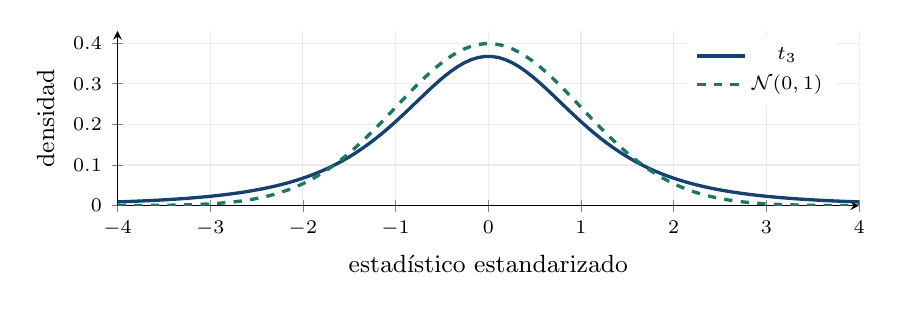
\begin{tikzpicture}
\begin{axis}[base,width=11cm,height=3.8cm,xmin=-4,xmax=4,ymin=0,ymax=.43,xlabel={estadístico estandarizado},ylabel={densidad},legend pos=north east]
\addplot[curva,domain=-4:4]{2/(pi*sqrt(3))*(1+x*x/3)^(-2)};\addlegendentry{$t_3$}
\addplot[verde,dashed,very thick,domain=-4:4]{exp(-x*x/2)/sqrt(2*pi)};\addlegendentry{$\Normal(0,1)$}
\end{axis}
\end{tikzpicture}
\caption{Estimar la escala produce colas Student más pesadas que las de una normal estándar.}
\end{figure}
\topic{Contrastes, predicciones y funciones de coeficientes}{s37}
Sea $\widehat\beta$ condicionalmente insesgado con matriz de covarianza
$V$. Para $R\in\R^{q\times k}$ fijo,
\[
\E[R\widehat\beta\mid X]=R\beta,\qquad
\Cov(R\widehat\beta\mid X)=RVR\T.
\]
Un contraste $c\T\widehat\beta$ tiene varianza
$\sum_jc_j^2V_{jj}+2\sum_{j<r}c_jc_rV_{jr}$.
Ignorar covarianzas equivale a cambiar esa varianza.

\begin{ejemplo}[Sumar y restar coeficientes correlacionados]
Con
$V=\begin{psmallmatrix}.625&-.375\\-.375&.625\end{psmallmatrix}$,
\[
\Var(\widehat\beta_1+\widehat\beta_2)=.5,\qquad
\Var(\widehat\beta_1-\widehat\beta_2)=2.
\]
Usar solo la diagonal daría $1.25$ en ambos casos.
\end{ejemplo}
\textbf{Media predicha frente a nueva observación.}
Para un nuevo regresor fijo $x_0\in\R^k$,
$\widehat m_0=x_0\T\widehat\beta$ tiene
\[
\E[\widehat m_0\mid X]=x_0\T\beta,\qquad
\Var(\widehat m_0\mid X)=x_0\T Vx_0.
\]
Si $y_0=x_0\T\beta+u_0$ y $u_0$ es independiente de la muestra,
de media cero y varianza $\sigma^2$,
\[
\Var(y_0-\widehat m_0\mid X)=\sigma^2+x_0\T Vx_0.
\]
La primera varianza mide incertidumbre de una media; la segunda agrega
el ruido irreducible de una observación nueva.
Para $X_0$ con varias filas,
$\Cov(X_0\widehat\beta\mid X)=X_0VX_0\T$.
Predicciones hechas con los mismos coeficientes están correlacionadas.

\textbf{Funciones no lineales.}
Si $g:\R^k\to\R^q$ es diferenciable y $\widehat\beta$ está cerca de
$\beta$,
\[
g(\widehat\beta)\approx g(\beta)+J_g(\widehat\beta-\beta),
\qquad \Cov(g(\widehat\beta)\mid X)\approx J_gVJ_g\T.
\]
A segundo orden, la esperanza de la coordenada $g_a$ satisface
\[
\E[g_a(\widehat\beta)\mid X]\approx
g_a(\beta)+\tfrac12\tr(H_{g_a}V)
\]
para estimación insesgada, bajo control del resto de Taylor.

\textbf{Exponenciales gaussianas: resultado exacto.}
Si $\widehat\beta\mid X\sim\Normal_k(\beta,V)$ y
$L_j=\exp(\widehat\beta_j)$, la función generadora da
\[
\E[L_j\mid X]=e^{\beta_j+V_{jj}/2},
\quad
\boxed{\Cov(L_j,L_r\mid X)=
e^{\beta_j+\beta_r+(V_{jj}+V_{rr})/2}(e^{V_{jr}}-1)}.
\]
Para $j=r$ se obtiene la varianza lognormal.
Asimismo, $e^{\widehat\beta_j-V_{jj}/2}$ es insesgado para $e^{\beta_j}$
si $V_{jj}$ es conocido. Sustituirlo por una estimación aleatoria no
mantiene automáticamente el resultado.
En una ecuación de logingresos, transformar coeficientes, transformar
predicciones y recuperar la media del ingreso son tres cálculos distintos.

\topic{MCO numérico: cada operación y cada covarianza}{s38}
Estimemos $y_i=\beta_0+\beta_1x_i+u_i$ con
\[
x=(0,1,2,3,4)\T,\quad y=(1,2,2,4,6)\T,\qquad
X=\begin{pmatrix}1&0\\1&1\\1&2\\1&3\\1&4\end{pmatrix}.
\]
Como $\sum x_i=10$, $\sum x_i^2=30$, $\sum y_i=15$ y
$\sum x_iy_i=42$,
\[
X\T X=\begin{pmatrix}5&10\\10&30\end{pmatrix},\quad
C=(X\T X)^{-1}=\frac1{50}\begin{pmatrix}30&-10\\-10&5\end{pmatrix}.
\]
Multiplicando por $X\T y=(15,42)\T$,
\[
\widehat\beta=
\begin{pmatrix}.6&-.2\\-.2&.1\end{pmatrix}
\begin{pmatrix}15\\42\end{pmatrix}
=\begin{pmatrix}.6\\1.2\end{pmatrix}.
\]
$\widehat y=(.6,1.8,3,4.2,5.4)\T$,
$\widehat u=(.4,.2,-1,-.2,.6)\T$ y
$\widehat u\T\widehat u=1.6$.
Así, $n-k=3$ y $\widehat\sigma^2=1.6/3=8/15$.

\textbf{Todos los momentos de los coeficientes.}
Bajo exogeneidad y homocedasticidad,
\[
\E[\widehat\beta_0\mid X]=\beta_0,\quad
\E[\widehat\beta_1\mid X]=\beta_1,\quad
V_\beta=\sigma^2\begin{pmatrix}.6&-.2\\-.2&.1\end{pmatrix}.
\]
Sustituir $\sigma^2$ por $8/15$ estima
\[
\widehat V_\beta=\begin{pmatrix}.32&-8/75\\-8/75&4/75\end{pmatrix},
\quad
\operatorname{se}(\widehat\beta_0)=\sqrt{.32},
\quad \operatorname{se}(\widehat\beta_1)=\sqrt{4/75}.
\]
Las filas de $A=CX\T$ son
\[
A=\begin{pmatrix}.6&.4&.2&0&-.2\\-.2&-.1&0&.1&.2\end{pmatrix}.
\]
Sumar cuadrados de cada fila reproduce $.6$ y $.1$; multiplicarlas
y sumar reproduce $-.2$. Esto verifica la covarianza por ponderaciones.

\begin{figure}[H]\centering
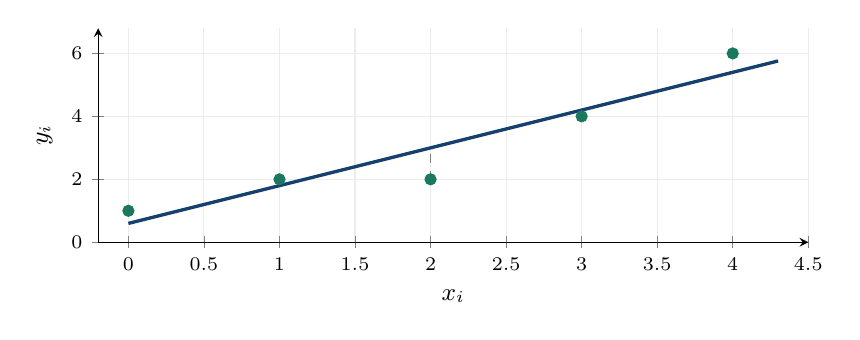
\begin{tikzpicture}
\begin{axis}[base,width=10.6cm,height=4.3cm,xmin=-.2,xmax=4.5,ymin=0,ymax=6.8,xlabel={$x_i$},ylabel={$y_i$}]
\addplot[curva,domain=0:4.3]{.6+1.2*x};
\addplot[only marks,mark=*,verde]coordinates{(0,1)(1,2)(2,2)(3,4)(4,6)};
\addplot[gray,dashed]coordinates{(2,2)(2,3)};
\end{axis}
\end{tikzpicture}
\caption{MCO minimiza errores verticales. PCA de $(x,y)$ usa otra distancia.}
\end{figure}
Para $x_0=3$, $\widehat m_0=.6+1.2(3)=4.2$.
Con $c=(1,3)\T$, $c\T Cc=.3$.
La varianza estimada de la media es $(8/15)(.3)=.16$;
la del error de una nueva observación es $(8/15)(1.3)=52/75$.
La diferencia es el ruido de esa nueva observación.

\topic{Heterocedasticidad, covarianza robusta y clústeres}{s39}
La expresión $V_\beta=A\Omega A\T$ permite identificar qué cambia
cuando los errores no tienen la misma varianza.
Para errores independientes con $\Var(u_i\mid X)=\sigma_i^2$,
\[
V_\beta=C\left(\sum_{i=1}^n x_ix_i\T\sigma_i^2\right)C,\qquad
C=(X\T X)^{-1}.
\]
HC0 sustituye las varianzas desconocidas por residuos al cuadrado:
\[
\boxed{\widehat V_{\mathrm{HC0}}
=C\left(\sum_i x_ix_i\T\widehat u_i^2\right)C}.
\]
HC1 multiplica por $n/(n-k)$; HC2 usa
$\widehat u_i^2/(1-h_{ii})$; HC3 usa
$\widehat u_i^2/(1-h_{ii})^2$, cuando $h_{ii}<1$.
Son estimadores de covarianza, no cambios de los coeficientes MCO.

\textbf{Por qué HC0 no es exacto en muestra finita.}
$\widehat u=M_Xu$ implica
\[
\E[\widehat u_i^2\mid X]=(M_X\Omega M_X)_{ii}
=\sum_a (M_X)_{ia}^2\sigma_a^2
\]
en el caso diagonal, generalmente distinto de $\sigma_i^2$.
Bajo homocedasticidad se reduce a $(1-h_{ii})\sigma^2$.
La consistencia robusta exige condiciones de momentos y que ninguna
observación domine el diseño.

\textbf{Agrupar observaciones dependientes.}
Supongamos $G$ grupos independientes entre sí, pero dependencia arbitraria
dentro de cada grupo. Si $X_g,u_g$ son los bloques,
\[
V_\beta=C\left(\sum_{g=1}^GX_g\T\Omega_gX_g\right)C.
\]
Definiendo la contribución vectorial $s_g=X_g\T\widehat u_g$,
\[
\boxed{\widehat V_{\mathrm{cl}}
=C\left(\sum_{g=1}^Gs_gs_g\T\right)C}.
\]
El producto exterior $s_gs_g\T$ agrega términos cruzados dentro del grupo:
\[
s_gs_g\T=\sum_{i\in g}\sum_{j\in g}x_ix_j\T\widehat u_i\widehat u_j.
\]
Una corrección usual de escala es
$\frac{G}{G-1}\frac{n-1}{n-k}$ para $G>1,n>k$,
pero no convierte el cálculo en una fórmula exacta universal.

\begin{ejemplo}[Dos registros del mismo individuo]
Para un modelo de media, dos errores de varianza $\sigma^2$ y covarianza
$\rho\sigma^2$ producen
\[
\Var((u_1+u_2)/2)=\sigma^2(1+\rho)/2.
\]
Ignorar su dependencia daría $\sigma^2/2$.
Si $\rho=.8$, la varianza verdadera es $1.8$ veces esa cifra.
\end{ejemplo}
Para un pooled con personas observadas repetidamente, agrupar por persona
permite esa dependencia dentro de la persona; añadir dummies de año y mes
no la elimina por definición.
La justificación asintótica requiere suficientes grupos independientes,
no solamente muchos registros.
Errores robustos cambian incertidumbre; no reparan por sí mismos
endogeneidad ni selección muestral.

\topic{GLS: blanquear errores y ganar eficiencia}{s40}
Supongamos $\E[u\mid X]=0$ y $\Cov(u\mid X)=\Omega\succ0$ conocida.
Mínimos cuadrados generalizados (GLS) minimiza
\[
Q_\Omega(b)=(y-Xb)\T\Omega^{-1}(y-Xb).
\]
Su gradiente es $-2X\T\Omega^{-1}(y-Xb)$.
Con $K_\Omega=X\T\Omega^{-1}X\succ0$,
\[
\boxed{\widehat\beta_G=K_\Omega^{-1}X\T\Omega^{-1}y},
\quad
\E[\widehat\beta_G\mid X]=\beta,
\quad \Cov(\widehat\beta_G\mid X)=K_\Omega^{-1}.
\]
La última igualdad resulta de multiplicar
$A_G\Omega A_G\T$, no de una hipótesis adicional.

\textbf{Blanqueamiento.}
Si $\Omega=LL\T$, transformamos $y^*=L^{-1}y$, $X^*=L^{-1}X$ y
$u^*=L^{-1}u$; $\Cov(u^*\mid X)=I_n$.
MCO sobre el modelo transformado coincide con GLS.
Con $\Omega=\sigma^2\diag(v_i)$, se divide cada fila por $\sqrt{v_i}$:
una observación de alta varianza recibe menor peso.

\begin{deduccion}
Un competidor lineal insesgado $B=A_G+D$ cumple $DX=0$.
El término cruzado es
$A_G\Omega D\T=K_\Omega^{-1}X\T D\T=0$.
Por tanto,
\[
\Cov(By\mid X)-\Cov(\widehat\beta_G\mid X)=D\Omega D\T\succeq0.
\]
Esta es la extensión de Gauss--Markov a una covarianza conocida general.
\end{deduccion}
\textbf{Información normal.}
Si $u\mid X\sim\Normal(0,\Omega)$, la logverosimilitud, salvo constantes, es
\[
\ell(b)=-\tfrac12\log\det\Omega
-\tfrac12(y-Xb)\T\Omega^{-1}(y-Xb).
\]
El score es $X\T\Omega^{-1}(y-Xb)$ y la información de Fisher
$I_\beta=K_\Omega$. La covarianza de GLS es su inversa y coincide
con la cota de información bajo las condiciones regulares del modelo.

\begin{ejemplo}[Estimar una media con distinta precisión]
$y_1=\mu+u_1$, $y_2=\mu+u_2$, independientes con varianzas $1$ y $4$.
Con $X=\ones_2$, GLS es
\[
\widehat\mu_G=\frac{y_1+y_2/4}{1+1/4}
=.8y_1+.2y_2,\quad \Var(\widehat\mu_G)=.8.
\]
MCO es $(y_1+y_2)/2$ y su varianza es $(1+4)/4=1.25$.
Si $y_1=1,y_2=3$, las estimaciones son $1.4$ y $2$.
\end{ejemplo}
\textbf{GLS factible.}
Cuando $\Omega$ se estima, $\widehat\beta_{\mathrm{FGLS}}$ ya no es
una transformación fija de $y$. Sus momentos exactos no son automáticamente
los de GLS conocido. Bajo convergencia apropiada de la matriz de pesos,
pueden coincidir en primer orden asintótico.
Si los pesos no representan bien $\Omega$, un sándwich calculado con
los errores estructurales puede ser necesario para la inferencia.


\begin{figure}[H]\centering
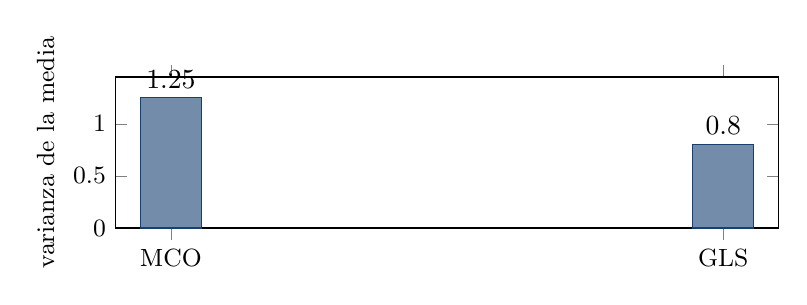
\begin{tikzpicture}
\begin{axis}[width=10cm,height=3.5cm,ybar,bar width=22pt,symbolic x coords={MCO,GLS},xtick=data,ymin=0,ymax=1.45,ylabel={varianza de la media},nodes near coords,point meta=y,tick label style={font=\small},label style={font=\small}]
\addplot[fill=azul!60,draw=azul]coordinates{(MCO,1.25)(GLS,.8)};
\end{axis}
\end{tikzpicture}
\caption{Dos observaciones de varianzas $1$ y $4$: ponderar por precisión reduce la varianza del estimador.}
\end{figure}
\topic{Regresión multivariada y matriz de coeficientes}{s41}
Ahora cada individuo tiene $q$ respuestas:
\[
Y=XB+U,\qquad
Y,U\in\R^{n\times q},\quad X\in\R^{n\times k},\quad B\in\R^{k\times q}.
\]
Supongamos $\E[U\mid X]=0$ y filas independientes con covarianza
$\Sigma_y\in\R^{q\times q}$.
La entrada $B_{ja}$ es el coeficiente del regresor $j$ en la respuesta $a$.
MCO minimiza $\norm{Y-XB}\F^2$ y la derivada matricial da
\[
\widehat B=(X\T X)^{-1}X\T Y=B+AU.
\]
Por tanto, $\E[\widehat B\mid X]=B$.

\textbf{Covarianza de cada par de coeficientes.}
Como $\Cov(U_{ia},U_{rb}\mid X)=\delta_{ir}(\Sigma_y)_{ab}$,
\[
\Cov(\widehat B_{ja},\widehat B_{\ell b}\mid X)
=\sum_{i,r}A_{ji}A_{\ell r}\delta_{ir}(\Sigma_y)_{ab}
=\boxed{C_{j\ell}(\Sigma_y)_{ab}},
\quad C=(X\T X)^{-1}.
\]
Vectorizando columnas,
\[
\boxed{\Cov(\vecop\widehat B\mid X)=\Sigma_y\otimes C}.
\]
La matriz tiene tamaño $kq\times kq$.
Para transformaciones fijas $R\widehat BT$,
\[
\Cov(\vecop(R\widehat BT)\mid X)
=(T\T\Sigma_yT)\otimes(RCR\T).
\]
Esto incluye contrastes conjuntos entre respuestas y regresores.

\begin{ejemplo}[Correlación entre ecuaciones]
Con $C=\begin{psmallmatrix}.6&-.2\\-.2&.1\end{psmallmatrix}$ y
$\Sigma_y=\begin{psmallmatrix}4&1\\1&9\end{psmallmatrix}$,
\[
\Var(\widehat B_{11})=2.4,\quad
\Var(\widehat B_{22})=.9,\quad
\Cov(\widehat B_{11},\widehat B_{22})=-.2.
\]
La covarianza entre el mismo regresor $2$ en las dos respuestas es
$C_{22}(\Sigma_y)_{12}=.1$.
\end{ejemplo}
\textbf{Distribución y residuos gaussianos.}
Si $U\mid X\sim\mathcal{MN}_{n,q}(0,I_n,\Sigma_y)$,
\[
\widehat B\mid X\sim\mathcal{MN}_{k,q}(B,C,\Sigma_y).
\]
Los residuos $\widehat U=M_XU$ tienen covarianza vectorizada
$\Sigma_y\otimes M_X$.
Con $\nu=n-k>0$,
\[
\widehat\Sigma_y=\frac{\widehat U\T\widehat U}{\nu},\qquad
\nu\widehat\Sigma_y\sim\mathcal W_q(\Sigma_y,\nu).
\]
$\widehat B$ y $\widehat\Sigma_y$ son independientes dado $X$.
Así se reúnen normal matricial, Wishart y regresión.

\textbf{Con más de un error de fila.}
Si $\Cov(\vecop U\mid X)=\Sigma_y\otimes\Omega$ con $\Omega\succ0$,
GLS multivariado es
$\widehat B_G=(X\T\Omega^{-1}X)^{-1}X\T\Omega^{-1}Y$ y
su covarianza vectorizada es
$\Sigma_y\otimes(X\T\Omega^{-1}X)^{-1}$.
Para una covarianza no separable se usa la transformación completa
$A$ en el modelo vectorizado.

\topic{CLT vectorial, método delta y sándwich}{s42}
Para vectores iid $z_i\in\R^d$ centrados, de covarianza finita $K$,
el teorema central del límite afirma
\[
\frac1{\sqrt n}\sum_{i=1}^nz_i\dto\Normal_d(0,K).
\]
Veamos el mecanismo para una combinación $a\T z_i$.
Su función característica cerca de cero cumple
$\varphi(t)=1-\tfrac12t^2a\T Ka+o(t^2)$.
Esta expansión se justifica con segundo momento finito y el resto
de Taylor controlado por integración.
La independencia da
\[
\varphi(t/\sqrt n)^n
=\left(1-\frac{t^2a\T Ka}{2n}+o(n^{-1})\right)^n
\longrightarrow e^{-t^2a\T Ka/2}.
\]
El límite es la característica normal. Hacerlo para todas las direcciones
$a$ identifica el límite vectorial.

\textbf{Delta.} Si
$\sqrt n(\widehat\theta-\theta)\dto\Normal_d(0,V)$
y $g:\R^d\to\R^q$ es diferenciable,
\[
\sqrt n\{g(\widehat\theta)-g(\theta)\}
=J_g\sqrt n(\widehat\theta-\theta)+o_{\Prob}(1)
\dto\Normal_q(0,J_gVJ_g\T).
\]
Es una afirmación de distribución, no por sí sola una prueba de convergencia
de esperanzas o varianzas. Para esos momentos se necesita control adicional
de colas, como integrabilidad uniforme.

\textbf{Estimadores definidos por ecuaciones.}
Supongamos que $\widehat\theta$ satisface
$n^{-1}\sum_i\psi(w_i,\widehat\theta)=0$,
con objetivo $\E[\psi(w,\theta_0)]=0$.
Sean
\[
J=\E\!\left[\frac{\partial\psi(w,\theta_0)}{\partial\theta\T}\right],
\quad K=\Cov(\psi(w,\theta_0)),
\quad J\text{ invertible}.
\]
Consistencia, un CLT y una expansión local uniforme dan
\[
0=\frac1n\sum_i\psi(w_i,\theta_0)+J(\widehat\theta-\theta_0)
+o_{\Prob}(n^{-1/2}).
\]
Despejando,
\[
\boxed{\sqrt n(\widehat\theta-\theta_0)
\dto\Normal(0,J^{-1}KJ^{-\mathsf T})}.
\]
La covarianza de primer orden del estimador es este sándwich dividido por $n$.

\begin{ejemplo}[MCO es un caso de esta fórmula]
Para $\psi_i=x_i(y_i-x_i\T\beta)=x_iu_i$,
$J=-Q$, $Q=\E[x_ix_i\T]$, y $K=\E[x_ix_i\T u_i^2]$ si
$\E[x_iu_i]=0$. Luego
\[
\sqrt n(\widehat\beta-\beta)\dto
\Normal(0,Q^{-1}KQ^{-1}).
\]
Con $\E[u_i^2\mid x_i]=\sigma^2$, $K=\sigma^2Q$.
\end{ejemplo}
Si los datos dependen, $K$ puede ser una covarianza de largo plazo que suma
covarianzas entre contribuciones. En clústeres se agrupan esas contribuciones
antes del producto exterior.
Esta estructura común permitirá analizar IV y SVR sin confundir sus
diferentes objetivos y supuestos.
\topic{Endogeneidad e identificación instrumental}{s43}
Para observaciones iid, $y_i=x_i\T\beta+u_i$ es una ecuación estructural \cite{hansen}.
Si $Q=\E[x_ix_i\T]\succ0$ y los momentos existen,
\[
\widehat\beta_{\mathrm{MCO}}-\beta
=\left(\frac1n\sum_i x_ix_i\T\right)^{-1}
\left(\frac1n\sum_i x_iu_i\right)
\pto Q^{-1}\E[x_iu_i].
\]
MCO es consistente para $\beta$ si $\E[x_iu_i]=0$.
Endogeneidad significa que este momento no es cero. Puede deberse a
variables omitidas, simultaneidad, medición con error u otros mecanismos.

\textbf{Instrumentos.}
Sea $z_i\in\R^\ell$, $\ell\ge k$.
Se propone sustituir la ortogonalidad respecto de $x_i$ por
\[
\E[z_iu_i]=0,\qquad
G=\E[z_ix_i\T]\in\R^{\ell\times k},\quad \rank(G)=k.
\]
La primera condición es validez de momentos; la segunda es relevancia
suficiente para identificar todas las coordenadas.
Las ecuaciones poblacionales son
$\E[z_iy_i]=G\beta$.
Si $G$ tiene rango completo, solo un $\beta$ las satisface.
Un intercepto requiere un instrumento constante junto con media cero
del error.

\begin{ejemplo}[Un modelo que separa validez y endogeneidad]
Con variables centradas,
\[
x=\pi z+v,\qquad y=\beta x+u,\qquad
\E[zv]=\E[zu]=0,\quad \Cov(v,u)=\tau\ne0.
\]
Si $\Var(z)>0$ y $\pi\ne0$,
\[
\Cov(z,x)=\pi\Var(z),\quad
\Cov(z,y)=\beta\pi\Var(z),
\]
\[
\boxed{\beta=\frac{\Cov(z,y)}{\Cov(z,x)}}.
\]
En cambio, si $z$ es incorrelacionado con $(v,u)$,
\[
\operatorname{plim}\widehat\beta_{\mathrm{MCO}}
=\beta+\frac{\tau}{\pi^2\Var(z)+\Var(v)}.
\]
El instrumento no necesita ser idéntico al regresor; necesita relacionarse
con él sin compartir el componente estructural del error.
\end{ejemplo}
\textbf{Variables omitidas, con cálculo explícito.}
Si $y=\beta x+\gamma w+\varepsilon$ y se omite $w$,
$u=\gamma w+\varepsilon$.
Con $\Cov(x,\varepsilon)=0$,
\[
\operatorname{plim}\widehat\beta_{\mathrm{MCO}}
=\beta+\gamma\frac{\Cov(x,w)}{\Var(x)}.
\]
Un instrumento válido debe cumplir el momento respecto de \emph{todo}
$u$, incluida la parte omitida.

\begin{cuidado}[Correlación no establece validez]
$\Cov(z,x)\ne0$ verifica relevancia escalar, pero no $\Cov(z,u)=0$.
La validez requiere una justificación del modelo y del origen del instrumento.
Que el ajuste de la primera etapa sea fuerte no demuestra exclusión.
Una muestra con $Z\T\widehat u$ pequeño tampoco prueba la condición poblacional.
\end{cuidado}
IV identifica parámetros de una ecuación bajo esos supuestos.
PCA y SVR tienen objetivos geométricos o predictivos distintos; no generan
instrumentos válidos por el solo hecho de reducir dimensión o predecir.

\topic{IV exacto: cocientes y momentos de muestra finita}{s44}
En identificación exacta, $\ell=k$ y $Z\T X$ invertible,
los momentos muestrales $Z\T(y-Xb)=0$ dan
\[
\boxed{\widehat\beta_{\mathrm{IV}}=(Z\T X)^{-1}Z\T y
=\beta+(Z\T X)^{-1}Z\T u}.
\]
El multiplicador depende de $X$, que puede depender del mismo $u$.
Por ello, $\E[Z\T u]=0$ no autoriza sacar la inversa de la esperanza:
\[
\E[\widehat\beta_{\mathrm{IV}}]-\beta
=\E[(Z\T X)^{-1}Z\T u]
\]
solo cuando existe esa integral.

\textbf{Una fórmula condicional que exige su propia hipótesis.}
Si se impusiera $\E[u\mid X,Z]=0$ y
$\Cov(u\mid X,Z)=\Omega$, entonces, con
$A_Z=(Z\T X)^{-1}Z\T$,
\[
\E[\widehat\beta_{\mathrm{IV}}\mid X,Z]=\beta,\qquad
\Cov(\widehat\beta_{\mathrm{IV}}\mid X,Z)=A_Z\Omega A_Z\T.
\]
Pero la endogeneidad que motiva IV generalmente viola la primera condición.
Este cálculo no es una prueba de insesgamiento del IV endógeno.

\begin{ejemplo}[Un momento instrumental cero y una media que no existe]
Considere un dato escalar con $z=1$, $x=1+v$, $u=v$,
$v\sim\Normal(0,1)$ y $y=\beta x+u$.
Entonces $\E[zu]=0$ y $\E[zx]=1$, pero
\[
\widehat\beta_{\mathrm{IV}}-\beta
=\frac{v}{1+v}=1-\frac1{1+v}.
\]
La densidad de $v$ es positiva cerca de $-1$.
La integral absoluta de $1/(1+v)$ diverge como
$\int_{-\varepsilon}^{\varepsilon}\abs t^{-1}\dd t$.
La esperanza ordinaria del estimador no existe.
Para $n$ datos iid, el cociente es
$\bar v/(1+\bar v)$: tiene el mismo problema para cada $n$ finito,
aunque $\bar v\pto0$ y el estimador sea consistente.
\end{ejemplo}
\textbf{Aproximación de sesgo de un cociente.}
Sea $R=A/B$, con medias $a,b$, $b\ne0$.
Las derivadas de $g(A,B)=A/B$ son
$g_{AA}=0$, $g_{AB}=-1/b^2$ y $g_{BB}=2a/b^3$.
Si las fluctuaciones son pequeñas y se controlan las colas,
\[
\E[R]\approx \frac ab
-\frac{\Cov(A,B)}{b^2}+\frac{a\,\Var(B)}{b^3}.
\]
Este Taylor no resuelve integrales divergentes cuando el denominador
puede acercarse a cero sin control suficiente.

\begin{idea}[La pregunta correcta para IV]
Primero se prueba identificación y consistencia con momentos instrumentales.
Después se deriva su distribución asintótica.
Los momentos finitos requieren un análisis adicional de los cocientes.
Consistencia y aproximación normal no implican automáticamente
insesgamiento ni una varianza finita para cada tamaño de muestra.
\end{idea}

\topic{2SLS: deducción de las dos etapas}{s45}
Si $\ell\ge k$, puede haber más momentos que coeficientes.
Con $Z\in\R^{n\times\ell}$ de rango $\ell$, proyectamos los regresores
sobre sus columnas:
\[
P_Z=Z(Z\T Z)^{-1}Z\T,\quad P_Z\T=P_Z,\quad P_Z^2=P_Z,\qquad
\widehat X=P_ZX.
\]
La primera etapa estima cada columna de $X$ por MCO con $Z$.
La segunda regresa $y$ sobre $\widehat X$.

\begin{deduccion}
La segunda etapa tiene coeficiente
\[
(\widehat X\T\widehat X)^{-1}\widehat X\T y.
\]
Por idempotencia,
$\widehat X\T\widehat X=X\T P_ZX$ y
$\widehat X\T y=X\T P_Zy$. Así,
\[
\boxed{\widehat\beta_2=(X\T P_ZX)^{-1}X\T P_Zy}.
\]
Se requiere $\rank(P_ZX)=k$.
Con $K_Z=X\T P_ZX$ y $A_2=K_Z^{-1}X\T P_Z$,
$A_2X=I_k$ y $\widehat\beta_2=\beta+A_2u$.
\end{deduccion}
\textbf{También minimiza una función de momentos.}
Los momentos sin normalizar son $Z\T(y-Xb)$.
Su cuadrado ponderado por $(Z\T Z)^{-1}$ es
\[
Q(b)=(y-Xb)\T Z(Z\T Z)^{-1}Z\T(y-Xb)
=(y-Xb)\T P_Z(y-Xb).
\]
Derivarlo da $X\T P_Z(y-Xb)=0$, exactamente la fórmula anterior.
Con $\ell=k$ y $Z\T X$ invertible, las ecuaciones implican
$Z\T(y-Xb)=0$ y 2SLS coincide con IV exacto.

\textbf{Qué residuo corresponde a la ecuación estructural.}
El residuo pertinente es
\[
\boxed{\widehat u=y-X\widehat\beta_2}.
\]
El residuo de la regresión mecánica de segunda etapa es
$\widetilde u=y-\widehat X\widehat\beta_2
=\widehat u+(X-\widehat X)\widehat\beta_2$.
Sus varianzas y sumas de cuadrados no son las mismas.
La matriz de covarianza IV debe usar los errores estructurales.

\begin{ejemplo}[El caso con un regresor centrado]
Con un instrumento centrado $z$ y regresor centrado $x$,
\[
P_z=\frac{zz\T}{z\T z},\quad
x\T P_zx=\frac{(x\T z)^2}{z\T z},\quad
x\T P_zy=\frac{(x\T z)(z\T y)}{z\T z}.
\]
Su cociente es $\widehat\beta=(z\T y)/(z\T x)$,
la fórmula de IV escalar.
\end{ejemplo}
No se debe aplicar la covarianza MCO de una segunda etapa ordinaria
como si $\widehat X$ fuera un diseño exógeno convencional.
El estimador utiliza instrumentos y regresores generados; su justificación
estadística se obtiene de la ecuación de momentos, que desarrollamos enseguida.

\topic{Covarianza asintótica de 2SLS}{s46}
Para datos iid y dimensiones $k,\ell$ fijas, supongamos
$\E[z_iu_i]=0$,
$Q_{zz}=\E[z_iz_i\T]\succ0$ y
$G=\E[z_ix_i\T]$ de rango $k$.
Definamos
\[
B=G\T Q_{zz}^{-1}G,\qquad
S_z=\E[z_iz_i\T u_i^2].
\]
La ley de grandes números aplicada a productos cruzados da
$n^{-1}X\T P_ZX\pto B$.
Usando la expresión algebraica del error,
\[
\sqrt n(\widehat\beta_2-\beta)
=\left(\frac{X\T P_ZX}{n}\right)^{-1}
\left(\frac{X\T Z}{n}\right)
\left(\frac{Z\T Z}{n}\right)^{-1}
\frac{Z\T u}{\sqrt n}.
\]
El último factor es una suma normalizada de $z_iu_i$.
Su CLT, unido a convergencia de los otros factores, produce
\[
\boxed{\sqrt n(\widehat\beta_2-\beta)
\dto\Normal_k(0,V_2)},
\]
\[
\boxed{V_2=B^{-1}G\T Q_{zz}^{-1}S_zQ_{zz}^{-1}GB^{-1}}.
\]
Cada coeficiente tiene varianza de primer orden $(V_2)_{jj}/n$;
cada par tiene covarianza $(V_2)_{jr}/n$.
Si $\E[u_i^2\mid z_i]=\sigma^2$,
$S_z=\sigma^2Q_{zz}$ y $V_2=\sigma^2B^{-1}$.

\textbf{Estimación robusta.}
Con $K_Z=X\T P_ZX$ y residuos estructurales $\widehat u_i$,
\[
\widehat V_{\mathrm{2,HC0}}
=K_Z^{-1}X\T Z(Z\T Z)^{-1}
\left(\sum_i z_iz_i\T\widehat u_i^2\right)
(Z\T Z)^{-1}Z\T XK_Z^{-1}.
\]
La misma expresión es $A_2\diag(\widehat u_i^2)A_2\T$.
En clústeres independientes, el centro se sustituye por
$\sum_g(Z_g\T\widehat u_g)(Z_g\T\widehat u_g)\T$.

\begin{ejemplo}[Relevancia escalar y precisión]
En $x=\pi z+v$, con $\Var(z)=q_z$, $\E[zu]=0$ y
$\E[u^2\mid z]=\sigma^2$,
\[
\operatorname{Avar}(\widehat\beta_{\mathrm{IV}})
=\frac{\sigma^2}{n\pi^2q_z}.
\]
Dividir $\pi$ por dos multiplica la varianza por cuatro.
\end{ejemplo}
\begin{cuidado}[El límite exige identificación estable]
Si $\pi=\pi_n$ se aproxima a cero al crecer $n$, la matriz límite puede
ser singular y la aproximación normal anterior falla.
Con instrumentos débiles, los cocientes pueden tener colas importantes
y la inferencia convencional puede ser inadecuada.
Estas fórmulas tampoco afirman que $\E[\widehat\beta_2]=\beta$
exactamente. Su centro asintótico es $\beta$ bajo los momentos válidos.
\end{cuidado}

\begin{figure}[H]\centering
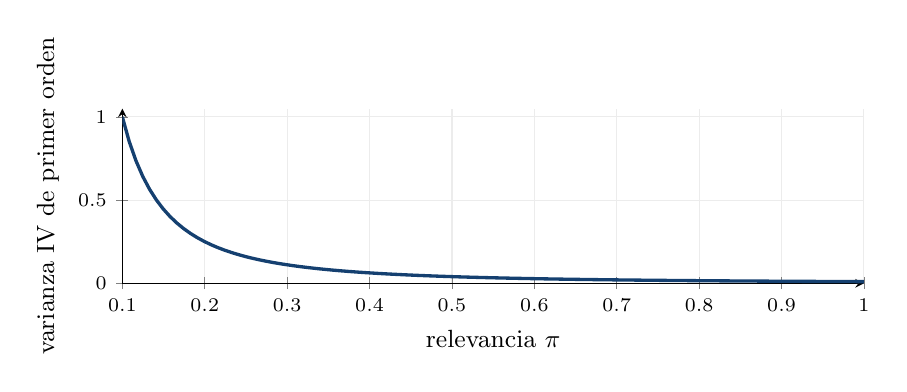
\begin{tikzpicture}
\begin{axis}[base,width=11cm,height=3.8cm,xmin=.1,xmax=1,ymin=0,ymax=1.05,xlabel={relevancia $\pi$},ylabel={varianza IV de primer orden}]
\addplot[curva,domain=.1:1]{.01/(x*x)};
\end{axis}
\end{tikzpicture}
\caption{Con $\sigma^2=\Var(z)=1,n=100$, la expresión $.01/\pi^2$ ilustra pérdida de precisión al debilitarse la primera etapa.}
\end{figure}
\topic{GMM y ponderación eficiente de momentos}{s47}
Sea $g_n(b)=n^{-1}\sum_i z_i(y_i-x_i\T b)\in\R^\ell$.
GMM minimiza $g_n(b)\T Wg_n(b)$ con $W\succ0$.
Definamos $G_n=Z\T X/n$ y $h_n=Z\T y/n$:
\[
g_n(b)=h_n-G_nb,\qquad
\nabla_b(g_n\T Wg_n)=-2G_n\T W(h_n-G_nb).
\]
Si $G_n\T WG_n$ es invertible,
\[
\boxed{\widehat\beta_W=(G_n\T WG_n)^{-1}G_n\T Wh_n}.
\]
Tomar $W=(Z\T Z/n)^{-1}$ produce 2SLS.

\textbf{Covarianza general.}
Bajo momentos válidos, identificación y condiciones de límite,
$G_n\pto G$ y $\sqrt n g_n(\beta)\dto\Normal(0,S_z)$.
Entonces, con $L_W=(G\T WG)^{-1}G\T W$,
\[
\sqrt n(\widehat\beta_W-\beta)\dto\Normal(0,V_W),
\quad
\boxed{V_W=L_WS_zL_W\T}.
\]
La matriz eficiente usa $W_*=S_z^{-1}$:
$V_*=(G\T S_z^{-1}G)^{-1}$.

\begin{deduccion}
$L_WG=L_*G=I_k$. Si $D=L_W-L_*$, $DG=0$ y
$L_*S_zD\T=(G\T S_z^{-1}G)^{-1}G\T D\T=0$.
Por tanto,
\[
V_W-V_*=DS_zD\T\succeq0.
\]
La eficiencia depende de ponderar por la covarianza de los momentos,
no por sus escalas aisladas. Con heterocedasticidad, 2SLS no tiene
necesariamente esa ponderación eficiente.
\end{deduccion}
En dos etapas de GMM se estima $S_z$ a partir de un estimador consistente,
$\widehat S_z=n^{-1}\sum_i z_iz_i\T\widehat u_i^2$,
y luego se usa su inversa. Un número suficiente de momentos independientes
y estabilidad de la estimación son necesarios.

\begin{ejemplo}[Dos mediciones de un mismo parámetro]
Si $G=(1,1)\T$ y $S_z=\diag(1,4)$, promediar por igual da
$V_W=(1+4)/4=1.25$.
Ponderar por $S_z^{-1}$ asigna pesos $.8,.2$ y da
$V_*=1/(1+1/4)=.8$.
La forma algebraica coincide con la media GLS.
\end{ejemplo}
\textbf{Sobreidentificación.}
Si $\ell>k$ y se usa ponderación eficiente,
\[
J_n=n\,g_n(\widehat\beta)\T\widehat S_z^{-1}g_n(\widehat\beta)
\dto\chi^2_{\ell-k}
\]
bajo validez conjunta y las condiciones regulares.
En coordenadas blanqueadas, estimar $k$ parámetros proyecta la fluctuación
normal de $\ell$ momentos sobre un subespacio de dimensión $k$;
el residuo tiene rango $\ell-k$.
No rechazar no prueba la validez de cada instrumento.
Con instrumentos débiles, demasiados momentos o covarianzas singulares,
esta derivación regular requiere revisión.

\topic{IV numérico: MCO, 2SLS y errores estructurales}{s48}
Construyamos seis filas usando vectores ortogonales:
\[
z_1=(-2,-1,0,0,1,2)\T,\quad z_2=(1,-1,0,0,-1,1)\T,
\]
\[
v=(0,0,1,-1,0,0)\T,\quad e=(1,-2,0,0,2,-1)\T.
\]
Son centrados y ortogonales por pares. Sea
$Z=[\ones,z_1,z_2]$, $x=z_1+v$, $u=v+e/2$ y
$y=\ones+2x+u$. La tabla es
\[
x=(-2,-1,1,-1,1,2)\T,\quad
y=(-2.5,-2,4,-2,4,4.5)\T.
\]
$X=[\ones,x]$. Los productos relevantes son
\[
Z\T Z=\diag(6,10,4),\quad
X\T X=\diag(6,12),\quad
X\T y=(6,26)\T.
\]
MCO da $(\widehat\beta_0,\widehat\beta_1)=(1,13/6)$.
El error comparte $v$ con $x$, y $x\T u=2$ explica esa diferencia.

\textbf{Primera y segunda etapas.}
Como $P_Zv=P_Ze=0$, $\widehat x=P_Zx=z_1$.
Luego
\[
X\T P_ZX=\diag(6,10),\quad
X\T P_Zy=(6,20)\T,\qquad
\boxed{\widehat\beta_2=(1,2)\T}.
\]
Los residuos estructurales son
$\widehat u=y-X\widehat\beta_2=u=(.5,-1,1,-1,1,-.5)\T$.
Su suma de cuadrados es $9/2$.
El residuo de segunda etapa mecánica es
$y-[\ones,z_1]\widehat\beta_2=3v+e/2$,
con suma de cuadrados $41/2$. Confundirlos multiplica el ruido calculado.

\textbf{Estimación de covarianzas.}
Bajo la fórmula homocedástica convencional y usando
$\widehat\sigma^2=(9/2)/(6-2)=9/8$,
\[
\widehat V_{2,\mathrm{hom}}
=\frac98\diag(1/6,1/10)=\diag(3/16,9/80).
\]
El operador de 2SLS es
\[
A_2=\begin{pmatrix}
1/6&1/6&1/6&1/6&1/6&1/6\\
-.2&-.1&0&0&.1&.2
\end{pmatrix}.
\]
La fórmula robusta HC0 da
\[
A_2\diag(\widehat u_i^2)A_2\T
=\boxed{\begin{pmatrix}1/8&0\\0&1/25\end{pmatrix}}.
\]
Por ejemplo, la varianza de la pendiente es
$[4(.25)+1(1)+1(1)+4(.25)]/100=.04$.

\begin{cuidado}[Qué demuestra este laboratorio]
Los números verifican el álgebra de MCO, proyecciones, 2SLS y sándwich.
La construcción tiene $Z\T u=0$ exactamente, pero una ortogonalidad
muestral elegida no demuestra validez causal poblacional.
Las matrices anteriores son estimaciones obtenidas con estos datos,
no una distribución exacta deducida de seis observaciones.
\end{cuidado}

\topic{SVR: pérdida insensible y objetivo poblacional}{s49}
Para datos $(x_i,y_i)$, SVR lineal propone $f(x)=w\T x+b$,
$w\in\R^p$, $b\in\R$, y penaliza el error
$r_i=y_i-f(x_i)$ mediante
\[
\rho_\varepsilon(r)=\max(0,\abs r-\varepsilon),\qquad \varepsilon\ge0.
\]
Errores dentro de $[-\varepsilon,\varepsilon]$ tienen costo cero;
fuera, el costo crece linealmente.
La función es convexa porque es el máximo de $0,r-\varepsilon,-r-\varepsilon$.

\textbf{Subgradiente.}
Una pendiente de soporte $s\in\partial\rho_\varepsilon(r)$ cumple
$\rho_\varepsilon(t)\ge\rho_\varepsilon(r)+s(t-r)$ para todo $t$.
Para $\varepsilon>0$,
\[
\partial\rho_\varepsilon(r)=
\begin{cases}
\{-1\},&r<-\varepsilon,\\[-2pt]
[-1,0],&r=-\varepsilon,\\
\{0\},&-\varepsilon<r<\varepsilon,\\
[0,1],&r=\varepsilon,\\
\{1\},&r>\varepsilon.
\end{cases}
\]
Si $\varepsilon=0$, se recupera $\abs r$ y el subgradiente en cero es
$[-1,1]$. No se usa una derivada ordinaria en los puntos angulosos.

\textbf{Problema regularizado.}
\[
\boxed{\min_{w,b}\frac12\norm w_2^2+
C\sum_{i=1}^n\rho_\varepsilon(y_i-w\T x_i-b)},\quad C>0.
\]
La norma controla complejidad en el espacio de características.
El intercepto no se penaliza en esta formulación.
Multiplicar todo el objetivo por una constante positiva no cambia
el minimizador.

\begin{figure}[H]\centering
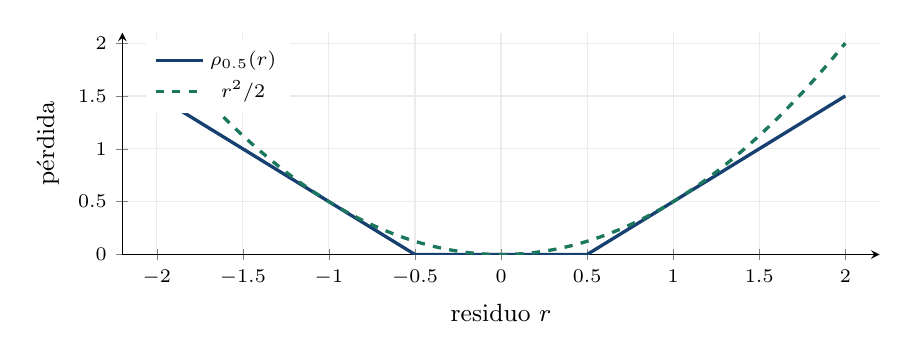
\begin{tikzpicture}
\begin{axis}[base,width=11.2cm,height=4.4cm,xmin=-2.2,xmax=2.2,ymin=0,ymax=2.1,xlabel={residuo $r$},ylabel={pérdida},legend pos=north west]
\addplot[curva]coordinates{(-2,1.5)(-.5,0)(.5,0)(2,1.5)};\addlegendentry{$\rho_{0.5}(r)$}
\addplot[verde,dashed,very thick,domain=-2:2]{.5*x*x};\addlegendentry{$r^2/2$}
\end{axis}
\end{tikzpicture}
\caption{La pérdida SVR tiene una banda plana y colas lineales.}
\end{figure}
\textbf{Qué función se estima.}
Sin penalización y sin restricciones funcionales, el minimizador poblacional
$a$ de $\E[\rho_\varepsilon(Y-a)\mid x]$ satisface, con densidad continua,
\[
\Prob(Y>a+\varepsilon\mid x)=\Prob(Y<a-\varepsilon\mid x).
\]
Para $\varepsilon=0$, es una mediana condicional.
Para ruido simétrico alrededor de una localización, esa localización
satisface la ecuación. En distribuciones asimétricas no tiene que coincidir
con $\E[Y\mid x]$. Por eso SVR no es MCO con otra fórmula de coeficientes.

\topic{SVR primal, dual y condiciones KKT}{s50}
Introducimos holguras $\xi_i,\xi_i^*\ge0$ \cite{smola}:
\[
\min_{w,b,\xi,\xi^*}\frac12\norm w^2+C\sum_i(\xi_i+\xi_i^*),
\quad
\begin{cases}
y_i-w\T x_i-b-\varepsilon-\xi_i\le0,\\
w\T x_i+b-y_i-\varepsilon-\xi_i^*\le0.
\end{cases}
\]
Para $w,b$ fijos, el menor costo de holguras es
$\rho_\varepsilon(y_i-w\T x_i-b)$.
Sea el lagrangiano, con multiplicadores no negativos,
\[
\begin{aligned}
\mathcal L={}&\tfrac12w\T w+C\sum_i(\xi_i+\xi_i^*)
+\sum_i\alpha_i(y_i-w\T x_i-b-\varepsilon-\xi_i)\\
&+\sum_i\alpha_i^*(w\T x_i+b-y_i-\varepsilon-\xi_i^*)
-\sum_i(\eta_i\xi_i+\eta_i^*\xi_i^*).
\end{aligned}
\]
La estacionariedad en variables primales da
\[
w=\sum_i(\alpha_i-\alpha_i^*)x_i,\quad
\sum_i(\alpha_i-\alpha_i^*)=0,\quad
C-\alpha_i-\eta_i=C-\alpha_i^*-\eta_i^*=0.
\]
Así, $0\le\alpha_i,\alpha_i^*\le C$.
Con $a=\alpha-\alpha^*$ y $K_{ij}=x_i\T x_j$, sustituir en
$\mathcal L$ elimina las variables primales y produce
\[
\boxed{\max_{\alpha,\alpha^*}
y\T a-\varepsilon\ones\T(\alpha+\alpha^*)
-\tfrac12a\T Ka},
\quad \ones\T a=0,\quad 0\le\alpha,\alpha^*\le C.
\]
La norma contribuye $+\tfrac12a\T Ka$ y los términos lineales en $w$
contribuyen $-a\T Ka$: de ahí el signo negativo final.

\textbf{Complementariedad KKT.}
Con $r_i=y_i-w\T x_i-b$,
\[
\alpha_i(r_i-\varepsilon-\xi_i)=0,\quad
\alpha_i^*(-r_i-\varepsilon-\xi_i^*)=0,
\]
\[
(C-\alpha_i)\xi_i=0,\qquad
(C-\alpha_i^*)\xi_i^*=0.
\]
Si $0<\alpha_i<C$, $\xi_i=0$ y
$b=y_i-w\T x_i-\varepsilon$.
Si $0<\alpha_i^*<C$, $b=y_i-w\T x_i+\varepsilon$.
Un punto estrictamente dentro del tubo tiene ambos multiplicadores cero.

\begin{idea}[Optimalidad y unicidad]
El problema es convexo y admite restricciones estrictamente factibles
tomando holguras suficientemente grandes. La condición de Slater \cite{boyd} garantiza
dualidad fuerte; factibilidad y KKT certifican optimalidad.
La penalización estrictamente convexa hace único $w$, pero el intercepto
o los multiplicadores pueden no ser únicos. Hay que fijar una regla de
selección antes de pedir la covarianza de un coeficiente no único.
\end{idea}
Para $\varepsilon>0$, un par óptimo no necesita tener
$\alpha_i,\alpha_i^*>0$ simultáneamente: disminuir ambos mantiene $a$ y
mejora el término de penalización. El caso $\varepsilon=0$ puede tener
representaciones duales redundantes.

\topic{Núcleos, Gram y representación de SVR}{s51}
Para una transformación de características $\phi(x)$ en un espacio
con producto interno, sustituimos $w\T x$ por
$\ip w{\phi(x)}$.
Un núcleo es $k(x,z)=\ip{\phi(x)}{\phi(z)}$.
La matriz de Gram $K_{ij}=k(x_i,x_j)$ es semidefinida positiva:
\[
c\T Kc=\sum_{i,j}c_ic_j\ip{\phi(x_i)}{\phi(x_j)}
=\norm{\sum_i c_i\phi(x_i)}^2\ge0.
\]
La covarianza de datos y una matriz Gram pueden ser positivas, pero
describen objetos distintos: variables frente a productos entre observaciones.

\textbf{Por qué solo hacen falta las características observadas.}
Descompongamos $w=w_\parallel+w_\perp$, con $w_\parallel$ en el
subespacio generado por $\phi(x_i)$ y $w_\perp$ ortogonal a él.
Todos los valores ajustados dependen únicamente de $w_\parallel$:
$\ip{w_\perp}{\phi(x_i)}=0$.
Por Pitágoras,
$\norm w^2=\norm{w_\parallel}^2+\norm{w_\perp}^2$.
El mínimo regularizado usa $w_\perp=0$:
\[
w=\sum_i a_i\phi(x_i),\qquad
\boxed{f(x)=\sum_i a_i k(x_i,x)+b}.
\]
El dual de la sección anterior funciona reemplazando el Gram lineal por
el Gram del núcleo.

\begin{ejemplo}[Núcleo cuadrático sin coordenadas misteriosas]
Para $x=(x_1,x_2)\T$, sea
$\phi(x)=(x_1^2,\sqrt2x_1x_2,x_2^2)\T$.
Entonces
\[
\ip{\phi(x)}{\phi(z)}
=x_1^2z_1^2+2x_1x_2z_1z_2+x_2^2z_2^2=(x\T z)^2.
\]
Una regresión lineal sobre $\phi(x)$ se convierte en una función cuadrática
de $x$. El núcleo evita construir esas coordenadas explícitamente.
\end{ejemplo}
\textbf{Núcleo gaussiano.}
Para $\gamma>0$,
\[
k(x,z)=e^{-\gamma\norm{x-z}^2}
=e^{-\gamma\norm x^2}e^{-\gamma\norm z^2}e^{2\gamma x\T z}.
\]
Expandir el último exponencial da
$\sum_{m\ge0}(2\gamma)^m(x\T z)^m/m!$.
Cada potencia es un producto interno de características tensoriales;
los coeficientes son no negativos. Multiplicar por las dos funciones
de escala y sumar preserva positividad. Así se justifica el núcleo.

\textbf{Centrar un Gram.}
Con $H=I-\ones\ones\T/n$, $K_c=HKH$ es el Gram de las
características centradas. La covarianza en características es
\[
\widehat C_\phi h
=\frac1{n-1}\sum_i\phi_{ci}\ip{\phi_{ci}}h.
\]
Sus autovalores positivos son los de $K_c/(n-1)$.
Esta es la conexión con kernel PCA: el mismo núcleo puede apoyar
una optimización de varianza o una pérdida de regresión, que son objetivos
diferentes.
El Gram no es la matriz de covarianza de los coeficientes duales;
esa incertidumbre procede de la aleatoriedad del entrenamiento.
\topic{SVR numérico: solución primal y dual}{s52}
Tomemos $(x_i,y_i)=(-1,-1),(0,0),(1,1)$, $C=1$ y
$\varepsilon=1/4$. Por simetría, probar $b=0$ es natural; las
condiciones KKT comprobarán que la solución es global.
Para $0\le w\le1$, el objetivo es
\[
J(w)=\tfrac12w^2+2\max(0,3/4-w).
\]
Si $w<3/4$, $J'(w)=w-2<0$; si $w>3/4$, $J'(w)=w>0$.
El mínimo se alcanza en
\[
\boxed{w=3/4,\quad b=0,\quad \xi_i=\xi_i^*=0},
\qquad J=9/32.
\]
Los extremos tienen residuos $-1/4,1/4$ y el punto central residuo cero.

\textbf{Certificado dual.}
El Gram lineal y los multiplicadores candidatos son
\[
K=\begin{pmatrix}1&0&-1\\0&0&0\\-1&0&1\end{pmatrix},\quad
\alpha=(0,0,3/8)\T,\quad \alpha^*=(3/8,0,0)\T.
\]
Entonces $a=\alpha-\alpha^*=(-3/8,0,3/8)\T$,
$\ones\T a=0$ y todos los multiplicadores pertenecen a $[0,1]$.
Además, $\sum_i a_ix_i=3/4=w$.
El valor dual es
\[
y\T a-\varepsilon\ones\T(\alpha+\alpha^*)-\tfrac12a\T Ka
=\frac34-\frac3{16}-\frac9{32}=\frac9{32}.
\]
Coincide con el primal; factibilidad y complementariedad verifican
optimalidad. El centro está estrictamente dentro del tubo y no es soporte.

\begin{figure}[H]\centering
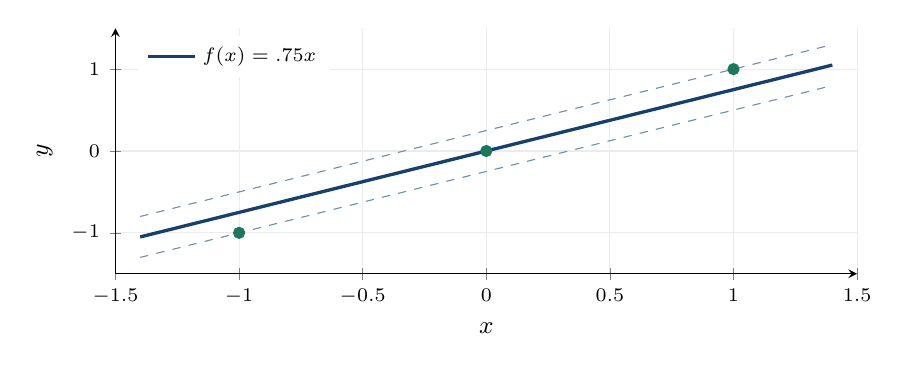
\begin{tikzpicture}
\begin{axis}[base,width=11cm,height=4.7cm,xmin=-1.5,xmax=1.5,ymin=-1.5,ymax=1.5,xlabel={$x$},ylabel={$y$},legend pos=north west]
\addplot[curva,domain=-1.4:1.4]{.75*x};\addlegendentry{$f(x)=.75x$}
\addplot[azul!60,dashed,domain=-1.4:1.4]{.75*x+.25};
\addplot[azul!60,dashed,domain=-1.4:1.4]{.75*x-.25};
\addplot[only marks,mark=*,verde]coordinates{(-1,-1)(0,0)(1,1)};
\end{axis}
\end{tikzpicture}
\caption{Los puntos extremos están en los bordes del tubo; el punto central tiene peso dual cero.}
\end{figure}
\textbf{Reducir el costo de holguras.}
Si $C=.2$, la misma función en $w<.75$ tiene derivada $w-.4$.
El mínimo es $w=.4,b=0$, con holgura $.35$ en cada extremo.
Los pesos duales son $a=(-.2,0,.2)\T$, saturados en $C$.
\[
J_{\mathrm{primal}}=.4^2/2+.2(.35+.35)=.22,
\quad
J_{\mathrm{dual}}=.4-.25(.4)-.4^2/2=.22.
\]
Este segundo caso muestra el compromiso entre norma y error.
No es una distribución de coeficientes: es una solución determinista
para datos observados. Para calcular sus momentos, hay que especificar
qué datos cambian entre muestras.

\topic{SVR: momentos exactos en un modelo resoluble}{s53}
Consideremos dos observaciones con $x_1=-1,x_2=1$:
\[
Y_1=b_0-\theta+u_1,\quad Y_2=b_0+\theta+u_2,\quad
u_1,u_2\stackrel{\mathrm{iid}}{\sim}\Normal(0,\sigma^2).
\]
Definamos $M=(Y_1+Y_2)/2$ y $D=(Y_2-Y_1)/2$.
Son conjuntamente normales, con
$M\sim\Normal(b_0,s^2)$, $D\sim\Normal(\theta,s^2)$,
$s^2=\sigma^2/2$, y $\Cov(M,D)=0$; son independientes.

\textbf{Resolver el estimador antes de promediarlo.}
Para $w$ fijo, elegir $b=M$ minimiza la suma de pérdidas por convexidad y
simetría. Fijamos esta regla si hay varios interceptos óptimos.
El objetivo se reduce a
$\tfrac12w^2+2C(\abs{D-w}-\varepsilon)_+$.
Con $L=2C$,
\[
\boxed{\widehat b=M,\quad
\widehat w=g(D)=\sign(D)\min\{(\abs D-\varepsilon)_+,L\}}.
\]
La solución se obtiene derivando en los intervalos lineales y comprobando
los bordes. Es umbralización seguida de saturación.

\textbf{Integrales truncadas que evalúan los momentos.}
Sea $M_r(a,b)=\E[D^r\ind_{\{a<D<b\}}]$,
$\alpha=(a-\theta)/s$, $\beta=(b-\theta)/s$,
$P=\Phi(\beta)-\Phi(\alpha)$, donde $\Phi$ es la acumulada estándar:
\[
\begin{aligned}
M_0(a,b)&=P,\\
M_1(a,b)&=\theta P+s\{\phi(\alpha)-\phi(\beta)\},\\
M_2(a,b)&=(\theta^2+s^2)P+
2\theta s\{\phi(\alpha)-\phi(\beta)\}
+s^2\{\alpha\phi(\alpha)-\beta\phi(\beta)\}.
\end{aligned}
\]
Se deducen cambiando $D=\theta+sZ$ e integrando
$z\phi(z)=-\phi'(z)$ y $z^2\phi(z)=\phi(z)-(z\phi(z))'$.
En extremos infinitos se usa $\phi(\pm\infty)=0$ y
$\lim_{\abs z\to\infty}z\phi(z)=0$.

Escribamos $A=(-\varepsilon-L,-\varepsilon)$,
$B=(\varepsilon,\varepsilon+L)$ y
$P_T=\Prob(D\le-\varepsilon-L)+\Prob(D\ge\varepsilon+L)$.
Entonces las cinco regiones de $g$ dan exactamente
\[
\begin{aligned}
m=\E[\widehat w]={}&-L\Prob(D\le-\varepsilon-L)
+M_1(A)+\varepsilon M_0(A)\\
&+M_1(B)-\varepsilon M_0(B)+L\Prob(D\ge\varepsilon+L),\\
q=\E[\widehat w^2]={}&L^2P_T+M_2(A)+2\varepsilon M_1(A)+\varepsilon^2M_0(A)\\
&+M_2(B)-2\varepsilon M_1(B)+\varepsilon^2M_0(B).
\end{aligned}
\]
Aquí $M_r(A)$ abrevia los extremos del intervalo $A$. Por independencia,
\[
\boxed{\E\begin{pmatrix}\widehat b\\\widehat w\end{pmatrix}
=\begin{pmatrix}b_0\\m\end{pmatrix},\quad
\Cov\begin{pmatrix}\widehat b\\\widehat w\end{pmatrix}
=\diag(s^2,q-m^2)}.
\]
Para $\theta=\sigma=C=1$, $\varepsilon=.25$,
$m\approx.780531$, $\Var(\widehat w)\approx.376600$:
hay sesgo $-.219469$. Los pesos duales netos son
$a=(-\widehat w/2,\widehat w/2)\T$ y su covarianza es
$\frac{q-m^2}{4}\begin{psmallmatrix}1&-1\\-1&1\end{psmallmatrix}$.
No se supuso una fórmula MCO para SVR.


\begin{figure}[H]\centering
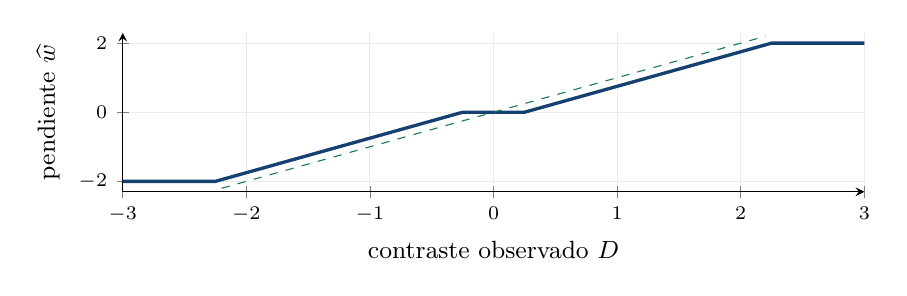
\begin{tikzpicture}
\begin{axis}[base,width=11cm,height=3.6cm,xmin=-3,xmax=3,ymin=-2.3,ymax=2.3,xlabel={contraste observado $D$},ylabel={pendiente $\widehat w$}]
\addplot[curva]coordinates{(-3,-2)(-2.25,-2)(-.25,0)(.25,0)(2.25,2)(3,2)};
\addplot[verde,dashed,domain=-2.2:2.2]{x};
\end{axis}
\end{tikzpicture}
\caption{$\varepsilon=.25,C=1$: SVR umbraliza y satura el contraste; MCO en dos puntos usaría $\widehat w=D$.}
\end{figure}
\topic{SVR: sándwich asintótico y remuestreo}{s54}
En dimensión finita, usemos $t=(1,x\T)\T$, $\theta=(b,w\T)\T$ y
$P=\diag(0,I_p)$. El objetivo normalizado es
\[
Q_n(\theta)=\frac\lambda2\theta\T P\theta+
\frac1n\sum_i\rho_\varepsilon(y_i-t_i\T\theta).
\]
Es equivalente al primal anterior cuando $\lambda=1/(nC)$.
Fijar $\lambda$ al crecer $n$ no equivale a fijar $C$.
Sea $\theta_\lambda$ el minimizador poblacional único y
$s_\varepsilon(r)=\sign(r)\ind_{\{\abs r>\varepsilon\}}$.
Con densidad condicional continua no hay masa en los bordes, y
\[
\E[g_i(\theta_\lambda)]=0,\qquad
g_i(\theta)=\lambda P\theta-t_i s_\varepsilon(y_i-t_i\T\theta).
\]

\textbf{Curvatura poblacional y dispersión del score.}
Aunque la pérdida muestral tiene ángulos, integrar contra una densidad
suaviza la ecuación poblacional.
Derivar las probabilidades de ambas colas produce
\[
\begin{aligned}
J={}&\lambda P+
\E\!\left[t_it_i\T
\{f_{Y\mid t}(t_i\T\theta_\lambda+\varepsilon\mid t_i)
+f_{Y\mid t}(t_i\T\theta_\lambda-\varepsilon\mid t_i)\}\right],\\
K={}&\Var\!\left(t_i s_\varepsilon(y_i-t_i\T\theta_\lambda)\right).
\end{aligned}
\]
Bajo consistencia, $J\succ0$, momentos suficientes y una expansión
estocástica uniforme de la ecuación no suave,
\[
\boxed{\sqrt n(\widehat\theta-\theta_\lambda)
\dto\Normal(0,J^{-1}KJ^{-1})}.
\]
La covarianza de primer orden es $J^{-1}KJ^{-1}/n$.
El objetivo puede estar sesgado respecto de un parámetro estructural:
el centro aquí es $\theta_\lambda$, no automáticamente $\beta$.

\begin{ejemplo}[SVR de localización sin penalización]
Si solo estimamos un intercepto y $Y=\mu+u$,
$u\sim\Normal(0,\sigma^2)$, entonces $\theta_0=\mu$.
Con $a=\varepsilon/\sigma$,
\[
J=2\phi(a)/\sigma,\quad K=2\{1-\Phi(a)\},\quad
\operatorname{Avar}(\widehat\mu)
=\frac{\sigma^2\{1-\Phi(a)\}}{2n\phi(a)^2}.
\]
Para $\varepsilon=0$, el estimador es una mediana y la varianza de primer
orden es $\pi\sigma^2/(2n)$, frente a $\sigma^2/n$ de la media normal.
\end{ejemplo}
\textbf{Estimación práctica de incertidumbre.}
$K$ se estima con productos exteriores de scores centrados.
$J$ necesita las densidades en los dos bordes, mediante un modelo o
una estimación de densidad consistente.
También puede usarse bootstrap de pares bajo condiciones regulares:
reentrenar en cada muestra, guardar $\widehat\theta^{*(b)}$ y calcular
\[
\widehat V_*=\frac1{B-1}\sum_{b=1}^B
(\widehat\theta^{*(b)}-\bar\theta^*)
(\widehat\theta^{*(b)}-\bar\theta^*)\T.
\]
En datos dependientes se remuestrean grupos o bloques.
Si se pretende incluir la elección de hiperparámetros en la incertidumbre,
esa elección debe repetirse dentro del remuestreo.
No unicidad, masas en los bordes, dimensión creciente o fronteras activas
inestables pueden invalidar el análisis regular: no existe una covarianza
cerrada universal de SVR.

\topic{Normal bayesiana, posterior y conexión con ridge}{s55}
Supongamos $y\mid\beta,X\sim\Normal_n(X\beta,\Omega)$,
$\Omega\succ0$ conocida, y un prior
$\beta\sim\Normal_k(m_0,V_0)$, $V_0\succ0$.
En esta interpretación, $\beta$ es aleatorio antes de observar $y$.
La posterior es proporcional a verosimilitud por prior:
\[
p(\beta\mid y,X)\propto
\exp\!\left[-\tfrac12\{
(y-X\beta)\T\Omega^{-1}(y-X\beta)
+(\beta-m_0)\T V_0^{-1}(\beta-m_0)\}\right].
\]
Expandir los cuadrados y reunir términos en $\beta$ da
\[
C_{\mathrm{post}}^{-1}=X\T\Omega^{-1}X+V_0^{-1},\qquad
m_{\mathrm{post}}=C_{\mathrm{post}}
(X\T\Omega^{-1}y+V_0^{-1}m_0).
\]
Completar el cuadrado transforma el exponente en
$(\beta-m_{\mathrm{post}})\T C_{\mathrm{post}}^{-1}
(\beta-m_{\mathrm{post}})$ más una constante:
\[
\boxed{\beta\mid y,X\sim\Normal_k(m_{\mathrm{post}},C_{\mathrm{post}})}.
\]

\textbf{La misma media vista como estimador frecuentista.}
Si $\beta$ se fija y se repite solamente el ruido de $y$,
\[
\E[m_{\mathrm{post}}\mid X]-\beta
=C_{\mathrm{post}}V_0^{-1}(m_0-\beta),
\]
\[
\boxed{\Cov(m_{\mathrm{post}}\mid X)
=C_{\mathrm{post}}X\T\Omega^{-1}X C_{\mathrm{post}}
=C_{\mathrm{post}}-C_{\mathrm{post}}V_0^{-1}C_{\mathrm{post}}}.
\]
Esta covarianza muestral del estimador no es la covarianza posterior
del parámetro. Condicionan sobre información distinta.

\textbf{Ridge como caso normal.}
Con $\Omega=\sigma^2I$, $m_0=0$ y $V_0=\tau^2I$,
$\lambda=\sigma^2/\tau^2$:
\[
m_{\mathrm{post}}=(X\T X+\lambda I)^{-1}X\T y,
\qquad C_{\mathrm{post}}=\sigma^2(X\T X+\lambda I)^{-1}.
\]
La media coincide con ridge, pero su covarianza frecuentista tiene
la expresión de la sección \ref{s32}.
Para una observación futura independiente,
\[
y_0\mid y,X,x_0\sim\Normal\!\left(
x_0\T m_{\mathrm{post}},\
\sigma^2+x_0\T C_{\mathrm{post}}x_0\right)
\]
en el caso homocedástico.

\begin{ejemplo}[Un solo parámetro]
Si $X\T X=4$, $\sigma^2=\tau^2=1$ y $\beta=2$,
$\lambda=1$ y $C_{\mathrm{post}}=1/5$.
La media posterior como estimador tiene esperanza $4(2)/5=1.6$,
sesgo $-.4$ y varianza muestral $4/25=.16$.
Su varianza posterior es $.2$.
\end{ejemplo}
Con un prior gaussiano sobre funciones y núcleo $K$,
la misma normal condicional da media
$k_* \T(K+\sigma^2I)^{-1}y$ y varianza
$k_{**}-k_*\T(K+\sigma^2I)^{-1}k_*$.
Esto es regresión gaussiana por núcleos; SVR no hereda esa posterior
por usar el mismo núcleo.


\begin{figure}[H]\centering
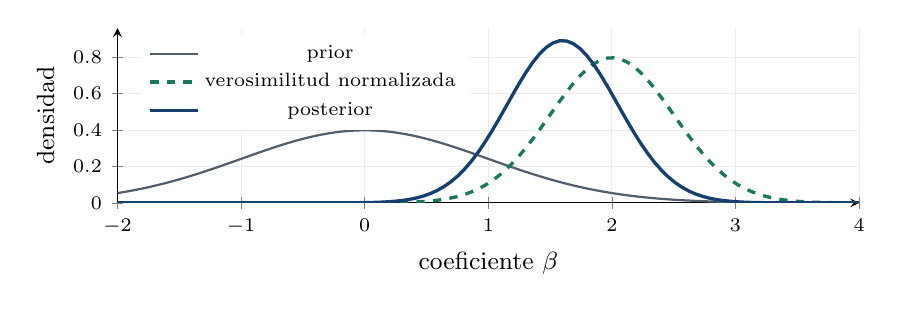
\begin{tikzpicture}
\begin{axis}[base,width=11cm,height=3.8cm,xmin=-2,xmax=4,ymin=0,ymax=.96,xlabel={coeficiente $\beta$},ylabel={densidad},legend pos=north west]
\addplot[gris,thick,domain=-2:4]{exp(-x*x/2)/sqrt(2*pi)};\addlegendentry{prior}
\addplot[verde,dashed,very thick,domain=-2:4]{exp(-(x-2)^2/.5)/sqrt(.5*pi)};\addlegendentry{verosimilitud normalizada}
\addplot[curva,domain=-2:4]{exp(-(x-1.6)^2/.4)/sqrt(.4*pi)};\addlegendentry{posterior}
\end{axis}
\end{tikzpicture}
\caption{Con $X^\mathsf T X=4,X^\mathsf T y=8,\sigma^2=\tau^2=1$, la posterior es $\Normal(1.6,.2)$.}
\end{figure}
\topic{Taller de integración y mapa de fórmulas}{s56}
\textbf{1. Cambiar coordenadas.}
Sea $\mu=(1,0)\T$, $\Sigma=\begin{psmallmatrix}4&2\\2&3\end{psmallmatrix}$
y $a=(1,-2)\T$.
Entonces $\E[a\T x]=1$ y
$\Var(a\T x)=4+4(3)-4(2)=8$.
Para $b=(1,1)\T$, $\Cov(a\T x,b\T x)=a\T\Sigma b=-4$.
No basta calcular por separado las varianzas de cada coordenada.

\textbf{2. Correlación sin independencia.}
Con $Z\sim\Normal(0,1)$ y $W=Z^2-1$,
$\E[W]=0$, $\Var(W)=3-1=2$ y $\Cov(Z,W)=\E[Z^3]-\E[Z]=0$.
El vector $(Z,W)$ no es normal conjunto, pues vive en una parábola.
Una covarianza diagonal aquí no implica independencia.

\textbf{3. Normal condicional.}
Para $\Sigma=\begin{psmallmatrix}4&2\\2&3\end{psmallmatrix}$ y media
$(1,0)\T$,
$x_1\mid x_2=t\sim\Normal(1+2t/3,8/3)$.
La varianza total es $8/3+(2/3)^2(3)=4$.

\textbf{4. Varianza de un contraste de MCO.}
Si $V=\sigma^2\begin{psmallmatrix}.6&-.2\\-.2&.1\end{psmallmatrix}$,
$\Var(\widehat\beta_0+2\widehat\beta_1)=
\sigma^2(.6-.8+.4)=.2\sigma^2$.
Su media es $\beta_0+2\beta_1$ bajo exogeneidad.
Con $\sigma^2$ desconocida se estima la escala; no se elimina la covarianza.

\textbf{5. Un modo pequeño de PCA puede importar para regresión.}
Si $x_1,x_2$ son independientes, de varianzas $100,1$, y
$y=x_2+u$ con $u$ independiente, PCA de una componente elige $x_1$.
Su mejor predictor lineal de $y$ es constante, mientras que usar $x_2$
elimina la varianza de la señal. Varianza de predictores y señal predictiva
son criterios distintos.

\textbf{6. Comparar dos métodos usando la misma muestra.}
Si $\widehat\theta_1=A_1y$ y $\widehat\theta_2=A_2y$,
\[
\Cov(\widehat\theta_1-\widehat\theta_2\mid X)
=(A_1-A_2)\Omega(A_1-A_2)\T.
\]
Sumar las dos covarianzas por separado omite
$A_1\Omega A_2\T+A_2\Omega A_1\T$.
La identidad se aplica a diferencias entre predicciones MCO, GLS y ridge
con matrices de transformación fijas.

\begin{center}\small
\begin{tabular}{@{}p{3.1cm}p{7.2cm}p{5cm}@{}}
\toprule
Objeto & Esperanza o centro & Covarianza o dispersión\\
\midrule
$Ax+b$ & $A\mu+b$ & $A\Sigma A\T$\\[4pt]
$\bar x$ iid & $\mu$ & $\Sigma/n$\\[4pt]
MCO, dado $X$ & $\beta$ si $\E[u\mid X]=0$ & $A\Omega A\T$\\[4pt]
Ridge, dado $X$ & $(X\T X+\lambda I)^{-1}X\T X\beta$ & $A_\lambda\Omega A_\lambda\T$\\[4pt]
2SLS & Centro asintótico $\beta$ con momentos válidos & Sándwich de sección \ref{s46}, dividido por $n$\\[4pt]
SVR & Objetivo $\theta_\lambda$; momentos finitos dependen del modelo & Exactos en sección \ref{s53}; sándwich regular en \ref{s54}\\
\bottomrule
\end{tabular}
\end{center}
\begin{idea}[La misma pregunta, en todas las dimensiones]
Define la aleatoriedad, verifica existencia de momentos, centra, transforma
y toma el producto exterior. Si el estimador es una transformación fija,
usa la identidad afín. Si depende no linealmente de los datos,
deriva su distribución o justifica una expansión local.
La notación matricial conserva todas las relaciones entre coeficientes.
\end{idea}

\clearpage
\section*{Compilación y referencias primarias}
\label{referencias}
\textbf{MiKTeX y VS Code.}
Este archivo usa la misma familia de paquetes del ejemplo: AMS,
\texttt{bm}, TikZ/PGFPlots, \texttt{tcolorbox}, \texttt{hyperref} y
tipografía Latin Modern. El idioma español se activa si
\texttt{spanish.ldf} está disponible; sin él, el contenido sigue siendo español
y el documento compila con la configuración básica.

\begin{enumerate}
\item Guarda el archivo con extensión \texttt{.tex} y codificación UTF-8.
\item En VS Code, abre ese archivo como documento principal de LaTeX Workshop.
\item Usa la receta pdfLaTeX y compila tres veces para actualizar índices
y referencias; alternativamente, ejecuta el comando siguiente.
\end{enumerate}
\begin{lstlisting}
latexmk -pdf -interaction=nonstopmode -halt-on-error Varianza_Covarianza_Matricial_MCO_IV_SVR.tex
\end{lstlisting}
No requiere Bib\TeX{}, Biber, archivos de imágenes ni ejecución de código
externo. MiKTeX debe tener instalados los paquetes citados; su gestor puede
instalarlos si falta alguno. El PDF ya compilado permite estudiar
sin configurar el editor.

\textbf{Sobre las demostraciones.}
Las deducciones y los ejemplos numéricos de este tratado están escritos
para seguir el cálculo de principio a fin. Las fuentes siguientes ofrecen
teoría de referencia y ampliaciones. Los momentos gaussianos y el
sándwich de estimadores se presentan con hipótesis explícitas:
la normalidad no se impone donde bastan segundos momentos, y no se
afirma una ley exacta donde solo se ha establecido un límite.

\begingroup\small
\renewcommand{\refname}{Fuentes para profundizar}
\begin{thebibliography}{9}\raggedright
\bibitem{mitnormal}
Massachusetts Institute of Technology. \textit{Fundamentals of Probability,
Lecture 14: Multivariate Normal Distributions}, 2018.
Notas oficiales de MIT OpenCourseWare.
\url{https://ocw.mit.edu/courses/6-436j-fundamentals-of-probability-fall-2018/resources/mit6_436jf18_lec14/}.

\bibitem{wishart}
Bishop, A. N.; Del Moral, P.; Niclas, A. (2017).
\textit{An Introduction to Wishart Matrix Moments}.
arXiv:1710.10864. Manuscrito de los autores.
\url{https://arxiv.org/abs/1710.10864}.

\bibitem{hansen}
Hansen, B. E. (2022). \textit{Econometrics}. Princeton University Press.
Página del autor, materiales y ruta a su texto.
\url{https://users.ssc.wisc.edu/~behansen/econometrics/}.

\bibitem{boyd}
Boyd, S.; Vandenberghe, L. (2004).
\textit{Convex Optimization}. Cambridge University Press.
Texto y recursos oficiales de los autores.
\url{https://web.stanford.edu/~boyd/cvxbook/}.

\bibitem{smola}
Smola, A. J.; Schölkopf, B. (2004).
\textit{A tutorial on support vector regression}.
Statistics and Computing, 14, 199--222.
DOI: 10.1023/B:STCO.0000035301.49549.88.
Versión alojada por el autor:
\url{https://alex.smola.org/papers/2004/SmoSch04.pdf}.
\end{thebibliography}
\endgroup
\end{document}
